\documentclass{article}
\usepackage[preprint,nonatbib]{neurips_2026}
\usepackage[T1]{fontenc}
\usepackage{amsmath,amssymb,amsthm,booktabs,graphicx,xcolor,flafter,hyperref,listings}
\definecolor{inklink}{RGB}{20,70,115}
\hypersetup{pdfauthor={Francois Chaubard and Astra (AI research collaborator)},colorlinks=true,linkcolor=inklink,citecolor=inklink,urlcolor=inklink,pdftitle={Weight-Space Programming and Gradient Optimization on Nonconvex Algorithmic Tasks}}
\newtheorem{theorem}{Theorem}
\newtheorem{proposition}[theorem]{Proposition}
\newcommand{\R}{\mathbb R}
\newcommand{\relu}{\operatorname{ReLU}}
\newcommand{\rank}{\operatorname{rank}}
\title{Weight-Space Programming and Gradient Optimization on Nonconvex Algorithmic Tasks}
\author{Francois Chaubard\\\href{mailto:fchaubar@stanford.edu}{\texttt{fchaubar@stanford.edu}}\And Astra\\{\small AI research collaborator (GPT-6 Astra)}}
% Computed from frozen evaluation files by revision/iteration_release.py.
\newcommand{\iterBetterE}{28}
\newcommand{\iterTieE}{35}
\newcommand{\iterWorseE}{24}
\newcommand{\oldPerfectE}{30}
\newcommand{\iterPerfectE}{30}
\newcommand{\vsGDE}{78}
\newcommand{\vsGLE}{77}
\newcommand{\iterBetterF}{27}
\newcommand{\iterTieF}{35}
\newcommand{\iterWorseF}{25}
\newcommand{\oldPerfectF}{30}
\newcommand{\iterPerfectF}{30}
\newcommand{\vsGDF}{78}
\newcommand{\vsGLF}{77}
\newcommand{\certIterE}{0}
\newcommand{\certIterF}{0}
\newcommand{\certGD}{0}
\newcommand{\certGL}{1}
\newcommand{\perfectGD}{0}
\newcommand{\perfectGL}{0}
\newcommand{\perfectPoolGD}{0}
\newcommand{\perfectPoolGL}{0}
\newcommand{\vsPoolGD}{78}
\newcommand{\vsPoolGL}{80}
\newcommand{\revCalls}{161}
\newcommand{\zeroStops}{60}
\newcommand{\exactStops}{60}
\newcommand{\patienceStops}{33}
\newcommand{\budgetStops}{81}
\newcommand{\latencySec}{51.7}
\newcommand{\outputTokens}{198,446}

\begin{document}
\maketitle
\begin{abstract}
The universal approximation theorem guarantees arbitrarily accurate approximation of continuous functions on compact domains with suitable activations and sufficient width. How should an optimizer find the weights, and which architecture should it use? We compare weight-space programming (WSP) with gradient optimization on ten algorithmic tasks. The fixed-network study covers 29 nonconvex task--architecture pairs and three random starts, using 3--50 coefficients in rectified linear, residual and recurrent networks. Astra, a pretrained language model, returns numerical weights in one reply or revises them using training and development feedback. Both examples-only WSP procedures match every extrapolation reference in the same 30 of 87 settings, including addition and running sums. Full-batch gradient descent using backpropagation achieves this in zero settings, as does descent followed by limited-memory Broyden--Fletcher--Goldfarb--Shanno (L-BFGS) refinement. Summing each task's mean raw extrapolation root mean squared error (RMSE) ranks the two iterative WSP conditions first among 14 evaluated pipelines. The examples-only sum falls from $1.06\times10^{12}$ to $2.03\times10^9$, driven mainly by improved Fibonacci predictions. The median scaled extrapolation error instead increases, and stored square-network coefficients show how central validation can favor a worse outer continuation. Thirty further requests let Astra choose the graph and coefficients from input/output examples, with extrapolation as the primary objective. Twenty-one proposals are exact on every outer input. Square uses a single product node with zero stored coefficients, while sine attains RMSE $7.79\times10^{-16}$. Two self-power proposals are invalid. We report coefficient storage, live tensor memory and arithmetic costs under the declared operation library, and reproduce prompts, returned graphs and public construction explanations.


\end{abstract}
\section{Introduction}
Universal approximation leaves open how to find the weights of a particular small network. Consider a network given twelve examples of addition. How closely do the returned weights fit those sums, and do the same weights still add correctly when both numbers are larger? We evaluate each solver on both questions. The unit of comparison is a \emph{task and architecture}: fixing addition as the target still leaves a choice between a linear map with two coefficients and a network with a trainable hidden layer. The former has a convex least-squares training loss. The latter can have several weight vectors that fit equally well and a much worse fit halfway between them.

\emph{Weight-space programming} (WSP) uses a specification or examples to assign numerical values directly to a network's weights. Our solver, GPT-6 Astra (Astra), receives the architecture, a random initial weight vector and labeled training examples. In \emph{one-shot WSP}, it returns numerical weights for every trainable coefficient in a single reply. In \emph{iterative WSP}, we start with those very weights, evaluate them on training and development examples, and invite up to three revisions. We keep a revision only if it improves the development loss, using the training loss to break a tie. Each procedure is run with examples only and with the generating formula supplied alongside the same examples.

Backpropagation (BP) computes a derivative; its use does not specify how to update the weights. Our first numerical baseline uses that derivative for full-batch gradient descent. Our second begins at the same gradient-descent endpoint and uses a limited-memory approximation to local curvature to refine it. We report both checkpoints. Additional comparisons use adaptive gradient steps and trust-region least squares. We evaluate the weights on the original training data and on disjoint tests inside and outside the original input range. For integer sequences both tests concern unseen later indices.

The benchmark covers four elementary functions, two arithmetic operations and four sequence or sorting tasks. For every included fixed-network task, architecture and training set we exhibit two weight vectors whose midpoint has higher loss than the average endpoint loss. This strict violation of the convexity inequality certifies that the empirical objective is nonconvex in its trainable parameters. It permits the comparison to include linear recurrent networks whose repeated trainable matrices make their losses nonconvex. We measure how often each method fits the observations more closely, how often that advantage carries beyond the observed range, and how the outcome changes with the number of parameters. The question concerns the quality of the returned weights at stated budgets. The tasks have known mathematical answers and allow direct checks of exactness.

We also ask Astra to choose the architecture from examples. Thirty further requests specify the observations, deployment domain and supported neural operations. Astra chooses the graph, its size and coefficients, with extrapolation accuracy as the primary objective and inference cost as the secondary objective. We evaluate every returned proposal and report its coefficient storage, activation memory and arithmetic cost.


\input{holistic_main}

\section{Related Work}
\paragraph{Comparing optimizers.} DeepOBS pairs tasks with specified networks and evaluates optimization methods on those problems \cite{schneider2019deepobs}. Schmidt et al.\ show experimentally how optimizer performance varies with task and tuning budget \cite{schmidt2021crowded}. We use small networks and few observations so that a language model can receive the entire parameter array, numerical solvers can use individual output derivatives, and some training optima can be computed independently. Our data also permit separate measurements of interpolation and extrapolation. We compare final predictions rather than speed at equal computation.

\paragraph{Constructing weights.} Algorithms have long been translated into neural weights, including recurrent computations \cite{siegelmann1994language,velez2026recurrent} and sorting in transformers \cite{lindner2023tracr}. Recent demonstrations used Astra to write game-policy weights and modify a pretrained language model \cite{takehi2026weightspace}. Other WSP studies tested bounded arithmetic and sorting through repeated proposals \cite{singh2026weightspace} or compiled numerical formulas into neural networks \cite{trimm2026benefits}. Our primary comparison fixes every graph, initial array, set of training labels and scoring objective before collecting its WSP responses. We report both the objective attained on those labels and accuracy on undisclosed test inputs.

\paragraph{Capacity and extrapolation.} Studies of arithmetic networks and algorithmic reasoning show how computation outside the training range depends on network structure \cite{trask2018nalu,madsen2020nau,xu2021extrapolation,velickovic2022clrs}. Universal approximation gives existence of a network that approximates a continuous function on a compact domain to a specified positive tolerance \cite{cybenko1989approximation,leshno1993approximation}. It leaves open the weights an optimizer will find and the size required to round an answer exactly. Vapnik--Chervonenkis dimension concerns the ability to realize every binary labeling of a point set \cite{bartlett2019vc}. We instead use lower bounds for the particular task and graph, including a bound on the number of linear pieces of a shallow square network. Floating-point arithmetic introduces additional expressivity and rounding questions \cite{park2024floating,hwang2025floating,park2026minimum,hwang2025robust}.

\paragraph{Selecting the architecture.}
Neural architecture search selects network structures using measured performance, as in the recurrent controller of Zoph and Le \cite{zoph2017nas}. Our additional experiment asks Astra to infer a rule from examples and return both a graph and its numerical coefficients in one response. We measure extrapolation and execution cost for each returned graph.


\section{Tasks, Architectures, and Optimization Methods}\label{sec:matched}
An \emph{architecture} specifies the operations and which scalar coefficients may change. A \emph{rectified linear unit} (ReLU) applies $R(u)=\max(0,u)$ to an input $u$. A multilayer perceptron (MLP) applies a sequence of affine maps (weighted sums plus biases) and activations. A recurrent neural network (RNN) carries a state vector from one step to the next and reuses the same weights at each step. Table~\ref{tab:architecture} lists every primary graph. The counts include all trainable biases and shared weights, with each stored scalar counted once.

\begin{table}[htbp]\centering\small
\caption{Architectures in the primary comparison. Sizes and parameter counts correspond left to right. A width counts hidden units or recurrent state coordinates. For sorting, size counts consecutive residual blocks, each acting on the same four wires.}\label{tab:architecture}
\begin{tabular}{@{}llrr@{}}\toprule
Target & Network & Sizes & Trainable parameters\\\midrule
Square, sine, positive self-power, & One hidden ReLU layer & $1,4,16$ & $5,14,50$\\
\quad hyperbolic tangent & with a direct input path & & \\
Addition, subtraction & Two-input ReLU MLP & $1,2,4$ & $5,9,17$\\
Running sum & Linear RNN with input & $1,2$ & $3,8$\\
Sort four numbers & Four-wire residual ReLU network & $4,5,6$ & $32,40,48$\\
Fibonacci numbers & Autonomous linear RNN & $1,2,3$ & $3,8,15$\\
Triangular numbers & Autonomous linear RNN & $2,3,4$ & $8,15,24$\\\bottomrule
\end{tabular}\end{table}

\paragraph{Graph definitions.}
The scalar targets are $x^2$, $\sin x$ in radians, $x^x$ on positive inputs, and the hyperbolic tangent $\tanh x$. For each hidden unit $j$ let $u_j,v_j,c_j$ denote its input slope, offset and output weight, and let $w$ be the width. With a direct linear path of slope $a$ and offset $b$, the scalar prediction is $ax+b+\sum_{j=1}^w c_j R(u_jx+v_j)$. Each unit introduces at most one change in slope, called a hinge. The addition and subtraction networks take two inputs, have no direct path and learn two input weights, a bias and an output weight per hidden unit, plus a final output bias.

For running sum the scalar input at tick $t$ is $x_t$. With a state of width $d$, a learned transition matrix $A$, input column $b$ and readout column $v$, the graph computes $h_t=Ah_{t-1}+b x_t$ from $h_0=0$ and predicts $v^\top h_t$ at every tick. Here $\top$ denotes transpose. For Fibonacci and triangular numbers the learned column $b$ is instead the initial state $h_0$, there are no inputs after initialization, and each tick applies $h_{t+1}=Ah_t$. At integer index $n\ge0$, Fibonacci numbers start at $0,1$ and each later term is the sum of its two predecessors. Triangular numbers equal $n(n+1)/2$. For sorting, the state $h$ initially holds the four inputs. Each block updates it to $h+vR(u^\top h)$ with its own learned four-component columns $u,v$. The final four values should give the original inputs in ascending order.

\paragraph{How we checked nonconvexity.}
For each of the 87 fixed-network settings, we exhibit two weight vectors whose midpoint has loss strictly greater than the average endpoint loss. Each witness uses two trainable coefficients that multiply along an active path. Swapping those coefficients preserves the endpoint prediction while changing the midpoint prediction. Exact rational evaluation on the actual training observations certifies the violation. Appendix~\ref{app:nonconvex-details} supplies the construction and its scope. The additional architecture-selection experiment can choose a different graph and is reported separately.



\paragraph{Initialization and observations.}
We used three random starts per task and architecture. Under Xavier-uniform initialization a layer with $p$ inputs and $q$ outputs draws its weights uniformly between $-\sqrt{6/(p+q)}$ and $\sqrt{6/(p+q)}$. Designated biases start at zero. All primary methods start with the same initial arrays and 12 central labeled inputs for targets with sampled inputs. A running-sum example is a length-six stream and a sorting example is a four-item list. The two integer sequences instead use the nine fixed indices 0 through 8. A new seed changes both the random training data and the weights where inputs are sampled. Test inputs are fixed across sizes and seeds. The three sizes (two for running sum) share a single WSP request, and the three integer-sequence starts share the same training indices.

\paragraph{Objective and methods.}
For observed scalar prediction $\hat y$ with label $y$, the scaled residual is $(\hat y-y)/\max(1,|y|)$. The common training objective is half the mean squared scaled residual, over every output coordinate. Both WSP prompts explicitly prioritize this objective and request extrapolation among similarly good fits. An \emph{endpoint} is the weight array a method returns using only the specified training information. The original four endpoints are the two WSP conditions and two numerical solvers.
\begin{itemize}
\item \textbf{One-shot WSP.} In the \emph{Examples only} condition, Astra sees the graph, initial weights, intended input range and examples. In \emph{Formula and examples}, it also sees the target rule. It returns one array per size in a single reply without tools or scoring feedback.
\item \textbf{Iterative WSP.} We retain both original information conditions. At each active size, Astra receives the selected weights, exact-match counts, errors and up to three worst labeled examples from each of the training and development sets. The development pool contains 256 new central inputs per sampled task and start, or indices 9--16 for the integer sequences. A revision replaces the current weights only when its development loss is strictly lower or, at equal development loss, its training loss is lower. An invalid proposal counts as a rejection. Each size stops when every training and development example is exact, after two consecutive rejections, or after three revision attempts. This is a finite stopping rule, not a guarantee of convergence. Requests for different cases may run concurrently. Each revision uses a fresh Astra session with the same task and selected weights; the prompt forbids tools, and we inspect the recorded events for tool use. Test inputs and scores never enter a revision. Appendix~\ref{app:feedback} describes the audit and controls.
\item \textbf{Gradient descent and gradient descent followed by L-BFGS.} Full-batch gradient descent uses the derivative computed by backpropagation and a training-loss line search for up to 800 updates. From that endpoint, the limited-memory Broyden--Fletcher--Goldfarb--Shanno method (L-BFGS) approximates curvature with ten recent pairs of weight and gradient changes, for up to 1,000 iterations \cite{liu1989limited}. We score the two endpoints separately.
\item \textbf{Adam followed by BFGS.} Adaptive moment estimation (Adam) scales each update using running averages of the gradient and its square \cite{kingma2015adam}. From Xavier we run 800 full-batch steps and then up to 1,000 iterations of the Broyden--Fletcher--Goldfarb--Shanno method (BFGS), which estimates local curvature from changes in gradients. The solver returns the lower training loss of its two stages.
\item \textbf{Trust-region least squares.} Starting at the identical Xavier weights, this solver uses the matrix of first derivatives of individual residuals (the Jacobian) to select local steps. It allows up to 250 residual evaluations followed by up to ten local polishing steps accepted on training loss. 
\end{itemize}
Appendix~\ref{app:limitedmemory} also reports L-BFGS directly from Xavier and from the 800-step Adam endpoint. The primary numerical solvers fit the original training labels. A separate control fits both gradient baselines to the entire labeled training and development pool.

The archive also scores the initial Xavier array. Astra brings pretrained knowledge of familiar formulas and operates under a different computational budget. Examples-only prompts disclose the deployment range and a task-specific graph. A match on visible information therefore controls the experiment more narrowly than a match on prior knowledge or compute.

\paragraph{Evaluation.}
We evaluate root mean squared error (RMSE) in target units over all scalar outputs. An exact prediction equals its reference in the standard 64-bit floating-point format (binary64), treating both signs of zero as equal. For running sums and sorting, one example counts as exact only if every coordinate matches. For the integer sequences we count matching indices on a single trajectory. Metrics are computed per endpoint before aggregation across starts. The central test uses fresh values in $[-3,3]$, and the outer test uses $[-10,-3]$ and $[3,10]$ with both signs for signed tasks. Positive self-power uses training inputs in $[0.02,3]$, central and development inputs drawn uniformly from $[0,3]$ (positive almost surely), and outer inputs in $[3,10]$. Each scalar evaluation has 2,048 samples per available outer side. Each arithmetic, sum or sorting test has 2,048 examples per split. The integer sequences use unseen indices 17--32 for early transfer and 33--64 for late transfer. The original one-shot study used 9--32 for early transfer. We preserve those scores separately because indices 9--16 are now used for feedback. Running sums in the primary comparison keep length six as magnitudes change. The supplement separately tests length 32. We report raw errors within tasks. For the aggregate ranking, we average raw outer RMSE over the sizes and starts of each task and then sum those ten task means. The supplementary plots also retain scaled errors and paired comparisons.

\section{Results}\label{sec:results}
\paragraph{Total error across all tasks.}
Figure~\ref{fig:holisticraw} ranks all 14 evaluated optimizer pipelines by summed raw extrapolation RMSE. Each task contributes its mean error across sizes and starts. Iterative WSP has the smallest sum in both information conditions, approximately $2.03\times10^9$. The examples-only one-shot sum is $1.06\times10^{12}$. More than 99.8\% of that one-shot total comes from Fibonacci, while positive self-power contributes 78.1\% of the iterative total. The aggregate therefore emphasizes errors on targets with large values. Figure~\ref{fig:holisticfull} shows the full range including divergent recurrent fits.

\paragraph{Central and extrapolation behavior.}
The median scaled error answers a different aggregation question. With examples alone, iteration reduces the held-out central or early median from 0.0214 to 0.000765, while the extrapolation median rises from 0.057 to 0.235. The scaled error divides each output residual by the larger of one and the target magnitude before computing RMSE. Figure~\ref{fig:priorscaledmedian} retains that view in the appendix. Table~\ref{tab:paired_methods} gives the eight primary endpoints.
\paragraph{What changes during revision?}
Figure~\ref{fig:wsp-learning} separates training fit, development feedback and untouched extrapolation across three revision opportunities. Development loss cannot rise under the selection rule, but neither training nor extrapolation error has that guarantee. With formulas and examples, median scaled outer RMSE falls from 0.0731 to 0.00590 after the first opportunity, then rises to 0.227 after the second. The final table alone hides this transient improvement. Test scores are retrospective and never select weights; stopped runs retain their last state. Appendix~\ref{app:learning-curves} separates proposed and retained weights and gives raw errors by task.
\input{learning_main}
\input{iterative_paired_table}
\paragraph{Does feedback improve extrapolation?}
With examples only, iterative WSP returned lower outer RMSE than one-shot WSP in \iterBetterE{} of 87 settings, the same RMSE in \iterTieE{}, and higher RMSE in \iterWorseE{}. With the formula supplied, the counts were \iterBetterF{}, \iterTieF{} and \iterWorseF{}. The number of settings exact on every outer reference changed from \oldPerfectE{} to \iterPerfectE{} with examples only and from \oldPerfectF{} to \iterPerfectF{} with the formula. In both conditions, the selected development loss fell strictly in 52 settings and tied in 35. In the examples-only condition the loss on the original training examples rose in 46, fell in six and tied in 35. The prompt requests exact unseen-domain outputs among similarly fitting solutions. The revision selector gives priority to central development loss. Figure~\ref{fig:prediction-curves} shows the computed functions for three fixed scalar cases. Across all six width-16 square networks, iteration moves every change of slope into $[-3,3]$, leaving affine predictions on the outer intervals. At input 10, one examples-only run changes its prediction from approximately 100 to 46.7. Appendix~\ref{app:prompts} reproduces the instructions, and Appendix~\ref{app:feedback} gives the coefficient-level diagnosis.

\paragraph{How does WSP compare with backpropagation-based updates?}
One-shot examples-only WSP gave lower outer RMSE than plain gradient descent in 75 of 87 settings and lower RMSE than gradient descent followed by L-BFGS in 75. For iterative examples-only WSP these counts were \vsGDE{} and \vsGLE{}, respectively. Neither training-only gradient procedure returned an entirely exact outer set. Refinement nevertheless mattered: at width two on subtraction, median RMSE fell from 0.831 after plain gradient descent to $1.44\times10^{-13}$ after L-BFGS. The two examples-only WSP procedures both matched all 2,048 inputs at each start. The original examples-only reply had lower outer RMSE than Adam followed by full BFGS in 73 settings and than trust-region least squares in 76. Its training loss was lower than Adam followed by BFGS in 79 settings. The full-information gradient control in Appendix~\ref{app:feedback} checks what changes if the numerical solvers also have access to the development labels.

\input{prediction_curves}

\paragraph{How large were the errors?}
Table~\ref{tab:focusouter} in the appendix gives the size of the errors and the exact-match counts at a specified network size for every task. Figures~\ref{fig:taskbars1}--\ref{fig:taskbars5} plot those same values for all eight methods. We chose sizes from the architecture and representability arguments: the largest tested scalar width, the two-unit arithmetic construction, and the smallest known sufficient real-arithmetic size for the sequence and sorting tasks. Table~\ref{tab:sizes_outer} gives all 29 pairs on the outer test. Tables~\ref{tab:sizes_dev} and~\ref{tab:sizes_train} report the central or early test and the training examples. No test score was used to pick an optimizer checkpoint.

\paragraph{Did the optimizer reach the global training minimum?}
For the four scalar tasks with one hidden unit we can compute the global optimum on the supplied labels in real arithmetic. After sorting the training inputs there are finitely many intervals for the change of slope. For each interval we fit the two affine pieces subject to continuity, also checking the boundaries, and take the smallest feasible loss. Appendix~\ref{app:optimizer} gives the rational arithmetic procedure for these same training data. This yields an independent benchmark in 12 settings. At an absolute tolerance of $10^{-10}$ above the certified optimum, one-shot examples-only WSP reached it in 1 of 12 settings, one-shot formula-and-examples WSP in 2, Adam followed by BFGS in 1, and trust-region least squares from Xavier in 5. Iterative WSP reached it in \certIterE{} and \certIterF{} settings in the two information conditions, respectively; gradient descent reached it in \certGD{} and gradient descent followed by L-BFGS in \certGL{}. This reverses the ordering of examples-only WSP and least squares seen in the outer-error comparisons.

\paragraph{What if least squares starts from the WSP weights?}
We took each of the 87 examples-only WSP arrays and applied the same trust-region solver and training-loss stopping rules used from Xavier. On the 12 certified fits this initialization brought the solver within tolerance of the global minimum in 12 of 12. Across the full benchmark the refinement lowered training loss by more than $10^{-10}$ in 22 settings. Among those 22, mean squared scaled outer error (with the same factor of one half as training) increased by more than $10^{-10}$ in 13 and decreased by more than $10^{-10}$ in nine. The 13 deteriorations also increased raw outer RMSE. The number of settings with every outer prediction exact stayed at 30. This two-stage experiment gives the refiner an additional model call through its starting weights. Zero extra numeric solver steps were available to the single-response WSP methods.


\section{Choosing the Architecture from Examples}\label{sec:free-architecture}
The fixed-network comparison asks each method to choose weights in a supplied graph. Here we ask Astra to choose the graph as well. Thirty independent requests cover ten tasks, with three requests per task using the original example sets. Each request supplies the input/output pairs, input shape and deployment domain. The prompt makes extrapolation the primary objective and asks for economical coefficient storage, inference memory and arithmetic among comparably accurate solutions.

The model can compose affine maps, rectified linear or hyperbolic tangent activations, multiplicative gates, recurrence, convolution and attention. It chooses every node, connection and coefficient within a maximum of 64 nodes and 4,096 stored coefficients. A convolution applies shared weights to local input windows. Attention uses input-dependent weights to combine values. These operations support multilayer, recurrent, convolutional and attention-based architectures. Direct multiplication and hyperbolic tangent can implement individual targets in this task set, so operator choice is part of the result.

We request one graph and a short construction explanation in each final answer. These are one-shot proposals; the calls use no tools or external numerical solver. The collector freezes all responses before a separate evaluator scores the unseen inputs. We count every request, including malformed graphs or nonfinite outputs. A floating-point operation (FLOP) is one scalar arithmetic operation. Comparisons and calls to exponential or hyperbolic tangent are counted separately. Memory includes stored 64-bit coefficients and peak live tensor storage for one input under the declared schedule. The memory count excludes operator-internal temporary arrays and Python or allocator overhead; it is not a measured process-memory footprint. Appendix~\ref{app:architecture_search} gives the full operator grammar, per-trial outcomes and archived explanations.
\input{architecture_main_results}


\section{Discussion and Limitations}
The benchmark asks two questions of the same weights. The training objective measures how well a method optimized the observations it received. Error on new input values or sequence indices measures whether those weights continued the rule. On an unseen input no optimizer can infer a unique continuation from central labels alone. For example, for any real number $a$, the functions $0$ and $aR(x-3)$ agree on the entire central interval $[-3,3]$. At $x=10$ their predictions differ by $7a$. Knowledge of the task family, the architecture and Astra's pretraining can all affect which continuation a solver chooses.

The fixed-network comparison covers ten deterministic numerical tasks, with up to 50 trainable coefficients. The architecture-selection experiment additionally changes the allowed graph and cost. Continuous tasks have three sampled training sets. Integer tasks have one training set and three initializations. Multiple sizes in the same WSP response share context. We give counts over these fixed cases and show each size. Population claims about optimizers in vision, language or general large-scale training require other workloads, models and budgets. The iterative method uses its development set for both feedback and selection. Three attempts cap the cost, and a rejected proposal can still perform better on unseen inputs. The original numerical baselines see fewer labels; we therefore also report an intervention giving the two gradient procedures the entire feedback pool. Neither design matches computation or pretraining. The examples-only condition still discloses the architecture and intended range, and there is no common unit equating an Astra inference to a gradient or Jacobian evaluation. Each hosted-model response is archived because the provider model name alone cannot guarantee its reproduction.

\paragraph{Which sizes are known to suffice?}
For a one-state running sum, setting all three weights to one returns every sum in the same addition order as the reference. Autonomous Fibonacci and triangular generators require minimum real-arithmetic state widths two and three, respectively, for their infinite sequences (Appendix~\ref{app:additional} and the realization argument in Appendix~\ref{app:proof}). For arithmetic, write $t=x_1+x_2$ or $x_1-x_2$. Even a single hidden unit can return $R(t+20)-20=t$ throughout the bounded real domain. The large intermediate offset can change its binary64 rounding. Two units give $R(t)-R(-t)=t$ without that offset. For the shallow scalar architecture the best possible uniform real error on square over $[-10,10]$ is $50/(w+1)^2$ at width $w$ (Appendix~\ref{sec:tasks}). A different deep graph returned by Astra provably rounds every square correctly on the outer shell; an engineered extension covers the full binary64 interval (Appendices~\ref{app:literal-square-certificate} and~\ref{app:fullsquare}). Those architectures and proofs give constructive bounds. They do not establish a minimal deep network for the smooth functions.

The supplementary edit theorem fixes a single output coordinate and counts how many initialized coefficients must change to implement a recurrence (Appendix~\ref{sec:front}). That question has a different unit of cost from the primary comparison, where each solver can change every weight. The supplement also studies a register machine, an abstract computer that updates integer registers according to conditional instructions. Its proof concerns unbounded exact integers; the reported binary64 runs test bounded executions (Appendix~\ref{app:machine}). Neither construction is counted as a win in the optimizer comparison.

\paragraph{Interpreting aggregate error and model size.}
The raw-RMSE sum gives each task one averaged contribution, but the target scale determines that contribution's magnitude. Large Fibonacci errors dominate many totals, especially at state widths that cannot exactly represent the recurrence. A rank under this measure differs from a rank under median scaled error. The architecture experiment measures the outputs and resource costs of 30 proposals. Its declared operations include a direct product and a hyperbolic tangent activation, so exactness on square and hyperbolic tangent can follow from one primitive. Zero stored coefficients attain the nonnegative coefficient-count lower bound. A smallest graph, smallest total storage or least arithmetic for every task would require additional proofs. Serialized graph storage is reported even when there are no stored coefficients.

\section{Conclusion}
Holding the task and graph fixed makes it possible to measure three different properties of an optimizer's final weights: how well they fit the displayed examples, how close they come to the right answer on new inputs, and whether they reproduce every reference exactly. Across the fixed-network benchmark, iterative WSP has the smallest summed raw extrapolation RMSE among the 14 evaluated pipelines. Its lower total coexists with regressions on individual tasks and an unchanged count of 30 fully exact settings. Allowing Astra to choose the graph yields 21 entirely exact extrapolation sets in 30 further requests, with costs determined by the permitted neural operations. Reporting the returned weights, input/output error and execution cost together exposes these tradeoffs.




\bibliographystyle{plain}
\bibliography{references}
\clearpage
\appendix\raggedbottom
\section{Final weights at each network size}\label{app:finalsizes}
Figures~\ref{fig:taskbars1}--\ref{fig:taskbars5} show the exact counts and errors from Table~\ref{tab:focusouter} as bars at one network size per task. Each task has its own error scale in the units of its output. Tables~\ref{tab:sizes_outer}--\ref{tab:sizes_train} then give all 29 task and architecture pairs on the extrapolation, central or early, and training sets.
\input{iterative_representative}
Even on addition and subtraction, whose generating rule is linear, training a two-layer network introduces nonconvexity in the weights. On these two tasks the width-two and width-four one-shot WSP networks in both information conditions reproduced every outer output in all 12 settings. At width two on subtraction, the least-squares optimizer had median outer RMSE $1.22\times10^{-15}$ and matched 769 of 2,048 inputs exactly at the median. At the same width on addition its median outer RMSE was 4.55. Training loss at or below $10^{-10}$ occurred in 17 of the 18 arithmetic least-squares fits. A threshold on training loss alone would miss both the near-exact subtraction and the large error on addition. The archived width-two one-shot WSP coefficients implement the target with a pair of opposite hidden weights in all six replies for each arithmetic task. Appendix~\ref{app:coefficients} decodes a literal reply and tests the symmetries of the scalar networks.

\input{task_panels}
\input{iterative_endpoint_tables}
\clearpage
\subsection{Validation feedback and additional gradient controls}\label{app:feedback}
\paragraph{What the model saw.} Each revision request reproduced the original specification and included only the active sizes, their incumbent weights, and diagnostics. For each size and split the model received the scaled loss, raw RMSE, whole-example exact count, and at most three non-exact inputs with the largest absolute scaled error on any coordinate. For each of those inputs it saw the target and current prediction. The 256 central development inputs were fixed within task and start and shared across sizes and prompt conditions. Integer indices 9--16 instead extended the original nine labels. Original one-shot replies, new prompts, replies, decisions and final vectors are retained. Appendix~\ref{app:repair} is a different experiment that allows a circuit description to change.
\paragraph{Stopping and selection.} The collector made \revCalls{} revision requests after the original 60 model calls. Their recorded median latency was \latencySec{} seconds per request, with \outputTokens{} output tokens in total; requests for different tasks ran concurrently. These requests produced 332 size-specific proposals, of which 217 were accepted; one width-16 square proposal had the wrong number of coefficients. None of the 161 requests used tools. The 174 size-by-condition trajectories share requests within an original task, start and prompt condition. Of those trajectories, \zeroStops{} were exact before any revision. At the end, \exactStops{} had stopped on exact training and development outputs, \patienceStops{} after two consecutive rejected proposals, and \budgetStops{} at the three-attempt cap. After all selections were frozen, a separate evaluator reconstructed the feedback from training and development data, checked every decision against the saved replies and then scored the selected weights. Table~\ref{tab:iterrounds} follows all 87 settings per condition through each revision opportunity. The cap limits what we can conclude about additional rounds.
\paragraph{What if gradient descent can use all feedback labels?} We separately fit both gradient procedures from the same Xavier start using the original training observations pooled with every feedback label, keeping both optimizer budgets and the test sets fixed. This gives the gradient solver 268 labeled examples per sampled task or 17 integer indices; Astra saw diagnostics and selected examples from that pool. The baseline therefore has access to more individual labels than Astra. With examples only, iterative WSP had lower outer RMSE than pooled-data gradient descent in \vsPoolGD{} settings and than its L-BFGS refinement in \vsPoolGL{} (out of 87). The pooled procedures matched every outer reference in \perfectPoolGD{} and \perfectPoolGL{} settings, respectively. Machine-readable files include training, feedback, independently held-out central or early, and outer scores for both pooled endpoints.
\paragraph{Independent test draw.} After the weight selection was frozen, we generated a second set of central and outer inputs using a new random seed. On the 69 settings with sampled inputs, the iterative-versus-one-shot outer RMSE comparison was 22 lower, 23 tied and 24 higher with examples only, and 20 lower, 23 tied and 26 higher with the formula supplied. The 18 integer settings have fixed target indices and are not repeated as independent draws. The companion data include the scores from both draws.

\begin{table}[htbp]\centering\small
\caption{What changed with each opportunity to revise? Each information condition keeps all 87 settings throughout. Attempted and accepted count individual size-specific proposals. After a size stops, its last retained weights carry forward. The last four columns are retrospective extrapolation scores; these scores were never shown to Astra. Exact counts settings in which every test prediction matched. Lower, equal and higher compare the retained outer RMSE with that setting\textquotesingle s one-shot outer RMSE.}\label{tab:iterrounds}
\begin{tabular}{@{}lrrrrrrr@{}}\toprule
Information & Round & Attempted & Accepted & Exact & Lower & Equal & Higher\\\midrule
Examples only & 0 & -- & -- & 30 & 0 & 87 & 0\\
 & 1 & 57 & 51 & 30 & 24 & 36 & 27\\
 & 2 & 57 & 32 & 30 & 28 & 35 & 24\\
 & 3 & 52 & 22 & 30 & 28 & 35 & 24\\
\midrule
Formula and examples & 0 & -- & -- & 30 & 0 & 87 & 0\\
 & 1 & 57 & 51 & 30 & 27 & 36 & 24\\
 & 2 & 57 & 34 & 30 & 27 & 35 & 25\\
 & 3 & 52 & 27 & 30 & 27 & 35 & 25\\
\bottomrule\end{tabular}\end{table}


\input{diagnosis}
\begin{figure}[htbp]\centering
\includegraphics[width=\linewidth]{square_continuation.pdf}
\caption{The actual width-16 square networks from the examples-only condition at random start 164. Training and development inputs lie in the central interval. The stored one-shot weights retain changes of slope outside that interval. Iteration concentrates all changes of slope inside it and extends an affine function into each outer interval. The curves explain this specific extrapolation regression.}\label{fig:square-continuation}
\end{figure}


\clearpage
\input{learning_appendix}
\clearpage
\subsection{Gradient descent and limited-memory optimization}\label{app:limitedmemory}
This subsection retains the original training-only gradient comparisons. Its early integer diagnostic uses the original indices 9--32. For a comparison with iterative WSP on untouched indices 17--32, see Table~\ref{tab:sizes_dev}. These fits use the same nonconvex networks, initial weights, training observations and loss as the main comparison. Plain full-batch gradient descent starts from Xavier and takes at most 800 updates. At each update it tries step size one and halves it until the training loss decreases sufficiently. Limited-memory Broyden--Fletcher--Goldfarb--Shanno (L-BFGS) uses the most recent ten pairs of changes in weights and gradients to approximate curvature. We run it with no parameter bounds for up to 1,000 iterations. Its reported endpoint has the lowest training loss among the supplied starting point and its accepted iterates. Selection uses training loss throughout.

We start L-BFGS from three separate points: the original Xavier weights, the gradient-descent endpoint, or the endpoint after 800 adaptive moment estimation (Adam) updates. The Adam checkpoint in Table~\ref{tab:limitedmemory_overview} is scored before refinement. The separate Adam--BFGS baseline applies full-memory BFGS after Adam. Each additional fit uses derivatives of the empirical loss obtained by backpropagation through the network. The complete records include optimizer termination, per-setting scores and fitted weights.

Tables~\ref{tab:limitedmemory_outer}, \ref{tab:limitedmemory_dev} and~\ref{tab:limitedmemory_train} give raw root mean squared error (RMSE) and exact matches at each tested size. Tables~\ref{tab:sizes_outer}--\ref{tab:sizes_train} give WSP and gradient results on the same outer and training inputs and on the current held-out central or early split, which uses indices 17--32 for the two integer sequences. Size denotes hidden width or the number of residual blocks for sorting. Slots count trainable scalar coefficients.

\begin{table}[htbp]\centering\small
\caption{Optimizer outcomes relative to all 87 matched settings. Near the optimum means an absolute loss gap of at most $10^{-10}$ to the independently certified minimum in the 12 one-hinge settings. The last column counts settings with strictly smaller outer raw RMSE for the first examples-only WSP response than for the named fit. Each setting contributes one comparison.}
\label{tab:limitedmemory_overview}
\setlength{\tabcolsep}{3.2pt}
\begin{tabular}{@{}lrrrrr@{}}
\toprule
 & \multicolumn{2}{c}{Observed training set} & Near the & Entire outer & WSP lower\\
\cmidrule(lr){2-3}
Method & Median loss & Loss $\leq 10^{-10}$ & optimum /12 & set exact /87 & RMSE /87\\
\midrule
Gradient descent & 0.0026 & 6 & 0 & 0 & 75 \\
Gradient descent $\to$ L-BFGS & $5.46\!\times\!10^{-4}$ & 32 & 1 & 0 & 75 \\
Adam (800 updates) & 0.00111 & 11 & 0 & 0 & 74 \\
Adam $\to$ L-BFGS & $5.34\!\times\!10^{-4}$ & 34 & 1 & 0 & 74 \\
L-BFGS from Xavier & $3.22\!\times\!10^{-5}$ & 37 & 3 & 0 & 71 \\
\bottomrule
\end{tabular}
\end{table}

\begin{table}[htbp]\centering\scriptsize
\caption{Exact counts and raw RMSE for gradient optimizers on the outer test. Continuous inputs have magnitudes from 3 to 10. Integer sequences use indices 33--64. Each entry is a median over the same three starts. Exact counts require every output of a stream or list, or one number at a given integer index. RMSE includes every scalar output in the target's units.}
\label{tab:limitedmemory_outer}
\setlength{\tabcolsep}{2pt}
\resizebox{\linewidth}{!}{\begin{tabular}{@{}lrr *{8}{r}@{}}
\toprule
 & & & \multicolumn{2}{c}{Gradient descent} &
 \multicolumn{2}{c}{\shortstack{Gradient descent\\then L-BFGS}} &
 \multicolumn{2}{c}{\shortstack{Adam\\then L-BFGS}} &
 \multicolumn{2}{c}{\shortstack{L-BFGS\\from Xavier}}\\
\cmidrule(lr){4-5}\cmidrule(lr){6-7}\cmidrule(lr){8-9}\cmidrule(l){10-11}
Target & Size & Slots & Exact & RMSE & Exact & RMSE & Exact & RMSE & Exact & RMSE\\
\midrule
Square & 1 & 5 & 0/4096 & 51.8 & 0/4096 & 51.8 & 0/4096 & 51.8 & 0/4096 & 51.8 \\
 & 4 & 14 & 0/4096 & 39.1 & 0/4096 & 39.1 & 0/4096 & 37.3 & 0/4096 & 40.1 \\
 & 16 & 50 & 0/4096 & 34.8 & 0/4096 & 33.5 & 0/4096 & 29 & 0/4096 & 28.5 \\
Sine & 1 & 5 & 0/4096 & 2.57 & 0/4096 & 2.57 & 0/4096 & 2.18 & 0/4096 & 2.56 \\
 & 4 & 14 & 0/4096 & 2.15 & 0/4096 & 2.45 & 0/4096 & 2.26 & 0/4096 & 2.57 \\
 & 16 & 50 & 0/4096 & 2.33 & 0/4096 & 2.52 & 0/4096 & 2.45 & 0/4096 & 2.81 \\
Positive self-power & 1 & 5 & 0/2048 & $1.58\!\times\!10^{9}$ & 0/2048 & $1.58\!\times\!10^{9}$ & 0/2048 & $1.58\!\times\!10^{9}$ & 0/2048 & $1.58\!\times\!10^{9}$ \\
 & 4 & 14 & 0/2048 & $1.58\!\times\!10^{9}$ & 0/2048 & $1.58\!\times\!10^{9}$ & 0/2048 & $1.58\!\times\!10^{9}$ & 0/2048 & $1.58\!\times\!10^{9}$ \\
 & 16 & 50 & 0/2048 & $1.58\!\times\!10^{9}$ & 0/2048 & $1.58\!\times\!10^{9}$ & 0/2048 & $1.58\!\times\!10^{9}$ & 0/2048 & $1.58\!\times\!10^{9}$ \\
Hyperbolic tangent & 1 & 5 & 0/4096 & 2.23 & 0/4096 & 2.23 & 0/4096 & 1.77 & 0/4096 & 1.94 \\
 & 4 & 14 & 0/4096 & 0.916 & 0/4096 & 0.618 & 0/4096 & 0.741 & 0/4096 & 0.551 \\
 & 16 & 50 & 0/4096 & 0.649 & 0/4096 & 0.343 & 0/4096 & 0.307 & 0/4096 & 0.195 \\
Addition & 1 & 5 & 0/2048 & 9.68 & 0/2048 & 9.68 & 0/2048 & 9.63 & 22/2048 & 5.19 \\
 & 2 & 9 & 0/2048 & 4.9 & 0/2048 & 4.2 & 31/2048 & 2.09 & 8/2048 & 5.48 \\
 & 4 & 17 & 0/2048 & 0.266 & 2/2048 & 0.266 & 0/2048 & 0.815 & 2/2048 & 0.0279 \\
Subtraction & 1 & 5 & 0/2048 & 4.92 & 30/2048 & 4.77 & 211/2048 & 4.46 & 449/2048 & 4.47 \\
 & 2 & 9 & 0/2048 & 0.831 & 14/2048 & $1.44\!\times\!10^{-13}$ & 63/2048 & 3.64 & 5/2048 & $6.49\!\times\!10^{-14}$ \\
 & 4 & 17 & 0/2048 & 0.754 & 2/2048 & 0.00435 & 4/2048 & $5.61\!\times\!10^{-13}$ & 1/2048 & $6.84\!\times\!10^{-13}$ \\
Running sum & 1 & 3 & 0/2048 & $7.02\!\times\!10^{-14}$ & 0/2048 & $7.02\!\times\!10^{-14}$ & 0/2048 & $2.27\!\times\!10^{-14}$ & 0/2048 & $3.48\!\times\!10^{-15}$ \\
 & 2 & 8 & 0/2048 & $1.01\!\times\!10^{-13}$ & 0/2048 & $1.01\!\times\!10^{-13}$ & 23/2048 & $1.95\!\times\!10^{-15}$ & 9/2048 & $2.72\!\times\!10^{-15}$ \\
Sort four & 4 & 32 & 29/2048 & 5 & 46/2048 & 5.86 & 32/2048 & 4.88 & 20/2048 & 4.81 \\
 & 5 & 40 & 26/2048 & 4.44 & 8/2048 & 6.09 & 17/2048 & 8.61 & 30/2048 & 3.93 \\
 & 6 & 48 & 0/2048 & 5.71 & 0/2048 & 5.52 & 0/2048 & 5.11 & 0/2048 & 5.77 \\
Fibonacci & 1 & 3 & 0/32 & $3.17\!\times\!10^{12}$ & 0/32 & $3.17\!\times\!10^{12}$ & 0/32 & $3.17\!\times\!10^{12}$ & 0/32 & $2.39\!\times\!10^{12}$ \\
 & 2 & 8 & 0/32 & $2.44\!\times\!10^{10}$ & 0/32 & 0.0715 & 0/32 & 0.0503 & 0/32 & 0.0257 \\
 & 3 & 15 & 0/32 & $4.94\!\times\!10^{11}$ & 0/32 & 0.0279 & 0/32 & 0.0152 & 0/32 & 0.24 \\
Triangular & 2 & 8 & 0/32 & $1.47\!\times\!10^{9}$ & 0/32 & $1.47\!\times\!10^{9}$ & 0/32 & $1.47\!\times\!10^{9}$ & 0/32 & $1.47\!\times\!10^{9}$ \\
 & 3 & 15 & 0/32 & $8.30\!\times\!10^{5}$ & 0/32 & $7.51\!\times\!10^{-8}$ & 0/32 & $3.15\!\times\!10^{-7}$ & 0/32 & $1.99\!\times\!10^{-8}$ \\
 & 4 & 24 & 0/32 & $1.59\!\times\!10^{7}$ & 0/32 & $6.88\!\times\!10^{-7}$ & 0/32 & $6.69\!\times\!10^{-7}$ & 0/32 & $5.65\!\times\!10^{-7}$ \\
\bottomrule
\end{tabular}}
\end{table}

\begin{table}[htbp]\centering\scriptsize
\caption{Exact counts and raw RMSE for gradient optimizers on the central or early-index test. Continuous inputs have central magnitudes up to 3. Integer sequences use unseen indices 9--32. Each entry is a median over the same three starts. Exact counts require every output of a stream or list, or one number at a given integer index. RMSE includes every scalar output in the target's units.}
\label{tab:limitedmemory_dev}
\setlength{\tabcolsep}{2pt}
\resizebox{\linewidth}{!}{\begin{tabular}{@{}lrr *{8}{r}@{}}
\toprule
 & & & \multicolumn{2}{c}{Gradient descent} &
 \multicolumn{2}{c}{\shortstack{Gradient descent\\then L-BFGS}} &
 \multicolumn{2}{c}{\shortstack{Adam\\then L-BFGS}} &
 \multicolumn{2}{c}{\shortstack{L-BFGS\\from Xavier}}\\
\cmidrule(lr){4-5}\cmidrule(lr){6-7}\cmidrule(lr){8-9}\cmidrule(l){10-11}
Target & Size & Slots & Exact & RMSE & Exact & RMSE & Exact & RMSE & Exact & RMSE\\
\midrule
Square & 1 & 5 & 0/2048 & 3.27 & 0/2048 & 3.27 & 0/2048 & 3.27 & 0/2048 & 3.27 \\
 & 4 & 14 & 0/2048 & 1.24 & 0/2048 & 1.24 & 0/2048 & 1.05 & 0/2048 & 1.24 \\
 & 16 & 50 & 0/2048 & 0.765 & 0/2048 & 0.575 & 0/2048 & 0.194 & 0/2048 & 0.309 \\
Sine & 1 & 5 & 0/2048 & 0.445 & 0/2048 & 0.445 & 0/2048 & 0.386 & 0/2048 & 0.381 \\
 & 4 & 14 & 0/2048 & 0.242 & 0/2048 & 0.109 & 0/2048 & 0.169 & 0/2048 & 0.137 \\
 & 16 & 50 & 0/2048 & 0.132 & 0/2048 & 0.0671 & 0/2048 & 0.111 & 0/2048 & 0.0902 \\
Positive self-power & 1 & 5 & 0/2048 & 5.59 & 0/2048 & 5.59 & 0/2048 & 5.59 & 0/2048 & 5.59 \\
 & 4 & 14 & 0/2048 & 5.59 & 0/2048 & 5.59 & 0/2048 & 3.62 & 0/2048 & 5.59 \\
 & 16 & 50 & 0/2048 & 3.81 & 0/2048 & 3.81 & 0/2048 & 4.45 & 0/2048 & 3.23 \\
Hyperbolic tangent & 1 & 5 & 0/2048 & 0.237 & 0/2048 & 0.237 & 0/2048 & 0.204 & 0/2048 & 0.209 \\
 & 4 & 14 & 0/2048 & 0.114 & 0/2048 & 0.133 & 0/2048 & 0.0923 & 0/2048 & 0.0412 \\
 & 16 & 50 & 0/2048 & 0.0421 & 0/2048 & 0.0368 & 0/2048 & 0.0266 & 0/2048 & 0.015 \\
Addition & 1 & 5 & 0/2048 & 2.43 & 0/2048 & 2.43 & 0/2048 & 2.44 & 97/2048 & 0.43 \\
 & 2 & 9 & 0/2048 & 0.248 & 1/2048 & 0.0323 & 51/2048 & 0.331 & 25/2048 & 0.258 \\
 & 4 & 17 & 0/2048 & 0.0161 & 9/2048 & 0.0156 & 4/2048 & 0.109 & 6/2048 & $1.34\!\times\!10^{-13}$ \\
Subtraction & 1 & 5 & 0/2048 & 0.304 & 185/2048 & 0.24 & 426/2048 & 0.152 & 539/2048 & 0.154 \\
 & 2 & 9 & 0/2048 & 0.167 & 65/2048 & $2.85\!\times\!10^{-14}$ & 134/2048 & 0.0952 & 8/2048 & $1.67\!\times\!10^{-14}$ \\
 & 4 & 17 & 0/2048 & 0.152 & 6/2048 & 0.00129 & 2/2048 & $1.11\!\times\!10^{-13}$ & 3/2048 & $1.50\!\times\!10^{-13}$ \\
Running sum & 1 & 3 & 0/2048 & $1.79\!\times\!10^{-14}$ & 0/2048 & $1.79\!\times\!10^{-14}$ & 0/2048 & $5.79\!\times\!10^{-15}$ & 1/2048 & $8.88\!\times\!10^{-16}$ \\
 & 2 & 8 & 0/2048 & $2.56\!\times\!10^{-14}$ & 0/2048 & $2.56\!\times\!10^{-14}$ & 21/2048 & $5.09\!\times\!10^{-16}$ & 8/2048 & $7.14\!\times\!10^{-16}$ \\
Sort four & 4 & 32 & 21/2048 & 1.32 & 43/2048 & 1.58 & 29/2048 & 1.28 & 10/2048 & 1.22 \\
 & 5 & 40 & 25/2048 & 1.11 & 9/2048 & 1.65 & 20/2048 & 2.26 & 35/2048 & 1.01 \\
 & 6 & 48 & 0/2048 & 1.44 & 0/2048 & 1.43 & 0/2048 & 1.3 & 0/2048 & 1.5 \\
Fibonacci & 1 & 3 & 0/24 & $5.66\!\times\!10^{5}$ & 0/24 & $5.66\!\times\!10^{5}$ & 0/24 & $5.66\!\times\!10^{5}$ & 0/24 & $5.66\!\times\!10^{5}$ \\
 & 2 & 8 & 0/24 & $2.73\!\times\!10^{3}$ & 0/24 & $7.67\!\times\!10^{-9}$ & 0/24 & $5.48\!\times\!10^{-9}$ & 0/24 & $3.12\!\times\!10^{-9}$ \\
 & 3 & 15 & 0/24 & $4.93\!\times\!10^{4}$ & 0/24 & $3.09\!\times\!10^{-9}$ & 0/24 & $1.78\!\times\!10^{-9}$ & 0/24 & $2.54\!\times\!10^{-8}$ \\
Triangular & 2 & 8 & 0/24 & $3.00\!\times\!10^{4}$ & 0/24 & $3.00\!\times\!10^{4}$ & 0/24 & $3.00\!\times\!10^{4}$ & 0/24 & $3.00\!\times\!10^{4}$ \\
 & 3 & 15 & 0/24 & $1.30\!\times\!10^{3}$ & 0/24 & $1.05\!\times\!10^{-9}$ & 0/24 & $5.78\!\times\!10^{-9}$ & 0/24 & $3.79\!\times\!10^{-10}$ \\
 & 4 & 24 & 0/24 & $5.09\!\times\!10^{3}$ & 0/24 & $1.38\!\times\!10^{-8}$ & 0/24 & $1.27\!\times\!10^{-8}$ & 0/24 & $9.38\!\times\!10^{-9}$ \\
\bottomrule
\end{tabular}}
\end{table}

\begin{table}[htbp]\centering\scriptsize
\caption{Exact counts and raw RMSE for gradient optimizers on the observed training set. Each setting has 12 labeled examples, or nine integer indices 0--8 for a number sequence. Each entry is a median over the same three starts. Exact counts require every output of a stream or list, or one number at a given integer index. RMSE includes every scalar output in the target's units.}
\label{tab:limitedmemory_train}
\setlength{\tabcolsep}{2pt}
\resizebox{\linewidth}{!}{\begin{tabular}{@{}lrr *{8}{r}@{}}
\toprule
 & & & \multicolumn{2}{c}{Gradient descent} &
 \multicolumn{2}{c}{\shortstack{Gradient descent\\then L-BFGS}} &
 \multicolumn{2}{c}{\shortstack{Adam\\then L-BFGS}} &
 \multicolumn{2}{c}{\shortstack{L-BFGS\\from Xavier}}\\
\cmidrule(lr){4-5}\cmidrule(lr){6-7}\cmidrule(lr){8-9}\cmidrule(l){10-11}
Target & Size & Slots & Exact & RMSE & Exact & RMSE & Exact & RMSE & Exact & RMSE\\
\midrule
Square & 1 & 5 & 0/12 & 2.8 & 0/12 & 2.8 & 0/12 & 2.8 & 0/12 & 2.8 \\
 & 4 & 14 & 0/12 & 0.792 & 0/12 & 0.792 & 0/12 & 0.434 & 0/12 & 1.07 \\
 & 16 & 50 & 0/12 & 0.296 & 0/12 & 0.29 & 0/12 & 0.00464 & 0/12 & 0.0291 \\
Sine & 1 & 5 & 0/12 & 0.399 & 0/12 & 0.399 & 0/12 & 0.399 & 0/12 & 0.325 \\
 & 4 & 14 & 0/12 & 0.0679 & 0/12 & 0.0327 & 0/12 & 0.0339 & 0/12 & 0.0339 \\
 & 16 & 50 & 0/12 & 0.0272 & 0/12 & 0.00294 & 0/12 & 0.0017 & 0/12 & $4.30\!\times\!10^{-4}$ \\
Positive self-power & 1 & 5 & 0/12 & 3.03 & 0/12 & 3.03 & 0/12 & 3.03 & 0/12 & 3.03 \\
 & 4 & 14 & 0/12 & 3.03 & 0/12 & 3.03 & 0/12 & 1.48 & 0/12 & 2.67 \\
 & 16 & 50 & 0/12 & 0.912 & 0/12 & 0.912 & 0/12 & 2.07 & 0/12 & 0.603 \\
Hyperbolic tangent & 1 & 5 & 0/12 & 0.211 & 0/12 & 0.211 & 0/12 & 0.21 & 0/12 & 0.175 \\
 & 4 & 14 & 0/12 & 0.0327 & 0/12 & 0.0279 & 0/12 & 0.0135 & 0/12 & 0.0107 \\
 & 16 & 50 & 0/12 & 0.0097 & 0/12 & 0.00527 & 0/12 & 0.00169 & 0/12 & 0.00115 \\
Addition & 1 & 5 & 0/12 & 1.72 & 0/12 & 1.72 & 0/12 & 1.72 & 0/12 & $2.55\!\times\!10^{-15}$ \\
 & 2 & 9 & 0/12 & 0.427 & 0/12 & $1.09\!\times\!10^{-13}$ & 0/12 & $6.11\!\times\!10^{-15}$ & 0/12 & $2.95\!\times\!10^{-15}$ \\
 & 4 & 17 & 0/12 & 0.00363 & 0/12 & $2.08\!\times\!10^{-14}$ & 0/12 & $2.86\!\times\!10^{-14}$ & 0/12 & $2.27\!\times\!10^{-14}$ \\
Subtraction & 1 & 5 & 0/12 & 0.0851 & 2/12 & $1.15\!\times\!10^{-15}$ & 2/12 & $5.62\!\times\!10^{-16}$ & 2/12 & $5.48\!\times\!10^{-16}$ \\
 & 2 & 9 & 0/12 & 0.106 & 0/12 & $5.02\!\times\!10^{-15}$ & 0/12 & $2.17\!\times\!10^{-15}$ & 0/12 & $1.53\!\times\!10^{-14}$ \\
 & 4 & 17 & 0/12 & 0.00799 & 0/12 & $3.14\!\times\!10^{-14}$ & 0/12 & $4.77\!\times\!10^{-14}$ & 0/12 & $5.56\!\times\!10^{-14}$ \\
Running sum & 1 & 3 & 0/12 & $1.25\!\times\!10^{-14}$ & 0/12 & $1.25\!\times\!10^{-14}$ & 0/12 & $5.07\!\times\!10^{-15}$ & 0/12 & $8.42\!\times\!10^{-16}$ \\
 & 2 & 8 & 0/12 & $2.03\!\times\!10^{-14}$ & 0/12 & $2.03\!\times\!10^{-14}$ & 0/12 & $4.84\!\times\!10^{-16}$ & 0/12 & $5.68\!\times\!10^{-16}$ \\
Sort four & 4 & 32 & 0/12 & 1.07 & 0/12 & 0.243 & 0/12 & 0.316 & 0/12 & 0.325 \\
 & 5 & 40 & 0/12 & 0.279 & 0/12 & 0.238 & 0/12 & 0.135 & 0/12 & 0.271 \\
 & 6 & 48 & 0/12 & 0.722 & 0/12 & 0.167 & 0/12 & 0.158 & 0/12 & 0.181 \\
Fibonacci & 1 & 3 & 0/9 & 7.53 & 0/9 & 6.78 & 0/9 & 5.68 & 0/9 & 8.91 \\
 & 2 & 8 & 0/9 & 0.00781 & 1/9 & $6.71\!\times\!10^{-15}$ & 1/9 & $1.35\!\times\!10^{-14}$ & 1/9 & $8.14\!\times\!10^{-15}$ \\
 & 3 & 15 & 0/9 & 0.0644 & 0/9 & $6.71\!\times\!10^{-15}$ & 0/9 & $5.76\!\times\!10^{-15}$ & 0/9 & $3.64\!\times\!10^{-14}$ \\
Triangular & 2 & 8 & 0/9 & 0.491 & 0/9 & 0.491 & 0/9 & 0.491 & 0/9 & 0.491 \\
 & 3 & 15 & 0/9 & 0.18 & 0/9 & $2.71\!\times\!10^{-14}$ & 0/9 & $1.15\!\times\!10^{-13}$ & 0/9 & $5.79\!\times\!10^{-14}$ \\
 & 4 & 24 & 0/9 & 0.214 & 0/9 & $2.44\!\times\!10^{-13}$ & 0/9 & $1.40\!\times\!10^{-13}$ & 0/9 & $1.01\!\times\!10^{-13}$ \\
\bottomrule
\end{tabular}}
\end{table}

\subsection{Alternative views of the optimizer comparison}\label{app:original-plots}
The following plots retain the earlier views of the same measured endpoints. Figure~\ref{fig:holisticfull} displays the complete range of summed raw errors. Figure~\ref{fig:priorscaledmedian} summarizes the median scaled error. Figures~\ref{fig:prioriterativepaired} and~\ref{fig:paired_endpoints} retain the original paired-comparison layouts. Their axes, legends and counts retain their original definitions.
\begin{table}[htbp]\centering\footnotesize
\caption{Raw-error totals and their dominant task. The total sums each task's mean RMSE across sizes and starts. The final two columns identify the largest task contribution and its share of that method's total. The graph-choosing proposals are evaluated separately in Appendix~\ref{app:architecture_search}.}\label{tab:holisticrank}
\begin{tabular*}{\linewidth}{@{\extracolsep{\fill}}rlrlr@{}}\toprule
Rank & Method & Raw-error sum & Largest contribution & Share \\\midrule
1 & Iterative WSP, formula + examples & $2.02598\times 10^{9}$ & Positive self-power & 78.12\%\\
2 & Iterative WSP, examples only & $2.02598\times 10^{9}$ & Positive self-power & 78.12\%\\
3 & L-BFGS from Xavier & $7.97356\times 10^{11}$ & Fibonacci & 99.74\%\\
4 & Trust-region least squares & $8.84785\times 10^{11}$ & Fibonacci & 99.77\%\\
5 & One-shot WSP, formula + examples & $9.38023\times 10^{11}$ & Fibonacci & 99.80\%\\
6 & One-shot WSP, examples only & $1.05832\times 10^{12}$ & Fibonacci & 99.80\%\\
7 & One-shot WSP + least squares, examples only & $1.05966\times 10^{12}$ & Fibonacci & 99.80\%\\
8 & Gradient descent, full feedback pool & $2.64518\times 10^{16}$ & Fibonacci & 100.00\%\\
9 & Gradient descent & $7.79363\times 10^{22}$ & Fibonacci & 100.00\%\\
10 & Adam, 800 updates & $1.83949\times 10^{30}$ & Fibonacci & 100.00\%\\
11 & Gradient descent + L-BFGS & $5.88992\times 10^{32}$ & Fibonacci & 100.00\%\\
12 & Gradient descent + L-BFGS, full feedback pool & $2.29320\times 10^{33}$ & Fibonacci & 100.00\%\\
13 & Adam + L-BFGS & $2.24329\times 10^{83}$ & Fibonacci & 100.00\%\\
14 & Adam + full BFGS & $8.22122\times 10^{232}$ & Fibonacci & 100.00\%\\
\bottomrule\end{tabular*}\end{table}

\input{holistic_full_range}
\clearpage
\input{prior_scaled_median}
\input{prior_iterative_comparisons}
\clearpage
\input{prior_task_comparisons}

\clearpage
\input{prompt_appendix}
\clearpage
\input{architecture_appendix}
\clearpage
\subsection{Nonconvexity witnesses for the fixed networks}\label{app:nonconvex-details}
\paragraph{How we checked nonconvexity.}
A convex training loss at the midpoint of any two weight vectors is at most the average of their losses. We check this inequality on the actual training examples. A linear recurrent network is linear in its input for fixed weights, but its input and readout weights multiply each other. For example, switch off the state transition and use just one state coordinate. Let its input weight be \(a\) and its readout weight be \(b\). Each tick then outputs \(ab\) times the current input. The pairs \((a,b)=(1,4)\) and \((4,1)\) have the same product, 4, while their midpoint \((5/2,5/2)\) has product \(25/4\). Reversing both readout signs if needed makes increasing the magnitude of this product increase the squared training loss. To see why, the initial slope of the loss as a function of the product at zero can have either sign. Choose the direction with nonnegative slope. Along that direction the loss is a strictly convex quadratic because at least one observed input is nonzero. The midpoint therefore has strictly greater loss than either endpoint.

The same construction works with the bias and readout of one active scalar rectifier, the input and output weights of one sorting block, or the initial state and readout of an autonomous sequence generator. All unused paths can be set to zero. In the sorter the original input still passes through its fixed identity connection. For the two autonomous tasks, a transition of one on the active coordinate keeps the output constant across the observed indices. Exact rational evaluation of the stored training data certifies 36 smooth-function settings (four tasks, widths 1, 4 and 16), six running sums (widths 1 and 2), nine four-input sorters (four, five or six blocks), and 18 sequence generators (Fibonacci widths 1--3 and triangular widths 2--4). Each size uses three starts. The sequence generators share their training labels across starts. Replaying the training code gives midpoint violations from 0.872 to 16.014 in units of training loss. The original 18 affine arithmetic settings and three memoryless sums minimize a weighted sum of squares of affine functions of their weights, a convex quadratic. Addition and subtraction on trainable rectifier networks of widths 1, 2 and 4 are a separate 18-setting experiment with their own midpoint certificates. A midpoint violation establishes the shape of the objective. Whether a solver reaches a better fit is a separate measurement.

\subsection{What the WSP responses encode}\label{app:coefficients}
\paragraph{What Astra returned.}
Each original one-shot model response was restricted to numeric arrays, with one full array per network size. Across 60 calls we recovered 174 arrays, all the requested shapes. The recording for each call contains one final message and zero tool actions. Relative to the supplied initialization, 3,142 of 3,252 stored scalars changed value. The prompts, original responses, run metadata and evaluated arrays permit an independent check of the computations encoded by the weights. The internal procedure by which Astra chose their numbers is unobserved.

For example, an examples-only addition request initialized a two-input, two-unit network with nine stored coefficients. Its returned array was $(1,1,-1,-1,0,0,1,-1,0)$. Read in the prompt's order, its hidden input rows are $(1,1)$ and $(-1,-1)$, both hidden biases are zero, the output weights are $(1,-1)$ and the output bias is zero. For inputs $(7,-9)$ the two rectified hidden values are $(0,2)$ and the output is $-2$. For inputs $(9,-7)$ the hidden values are $(2,0)$ and the output is $2$. The complete array thus implements $R(t)-R(-t)$ for the sum $t$. All 12 width-two arithmetic replies across the two tasks, both information conditions and three starts implement this sign pairing. The coefficient audit in the research bundle gives the prompt and reply paths for every case.

To check whether the scalar networks preserved a known symmetry, we evaluated each stored binary64 weight as an exact rational number. A one-layer scalar ReLU network gives an affine function between consecutive hidden-unit breakpoints. Its deviation from odd symmetry, $f(x)+f(-x)$, is therefore affine between those breakpoints and their reflections. Its maximum absolute value on $[-10,10]$ occurs at a breakpoint or an interval endpoint. None of the 18 sine arrays or 18 hyperbolic-tangent arrays was exactly odd on this interval. For sine specifically, 16 of 18 networks gave a nonzero value at zero. The remaining two failed the sign-reversal test at $1$ and $-1$. The analogous check for the even square target found zero exactly even arrays out of 18. These are symmetry tests on the returned coefficients, distinct from prediction tests in rounded arithmetic. The experiment varied task, architecture and formula access. The effect of a rule's familiarity to Astra remains open.

\paragraph{Does feedback restore symmetry?} Among the 18 sine networks across both information conditions, the exact symmetry test passed for none of the one-shot networks and 8 of the iteratively selected networks. For square, 0 one-shot and 11 iterative networks were exactly even; for hyperbolic tangent, 0 and 8 were exactly odd (out of 18 each). These statements concern the real function represented by the stored weights over $[-10,10]$.


\clearpage
\section{Numerical conventions for the additional studies}\label{app:numerics}
The primary benchmark uses the named NumPy numerical-library operation or an integer recurrence converted to binary64 as its reference. In the supplementary elementary-function experiments, the MPFR library for multiple-precision floating-point computation supplies correctly rounded mathematical values \cite{mpfr}. \emph{Correct rounding} returns the representable number nearest the exact mathematical result, choosing the one with an even last significand bit in a tie. The \emph{significand} holds the significant binary digits and the exponent gives their scale. Normal binary64 numbers have 53 significant bits. A dyadic rational is an integer divided by a power of two: for example, $3/8$ is exactly $0.011$ in binary. Every finite binary64 number has this form.

A \emph{unit in the last place} (ULP) is one step in the last stored digit at a given scale \cite{goldberg1991}. We measure ULP distance by counting adjacent representable values, treating both signs of zero as equal. At $1$, for example, the next larger number is $1+2^{-52}$ and the next smaller number is $1-2^{-53}$. Both have distance one under this convention. The mean scaled absolute error averages each absolute prediction error divided by the larger of one and the absolute reference value. A parameter \emph{slot} stores one scalar even if it is zero. An \emph{edit} changes one stored scalar from its initialized value. An \emph{operation} is an executed arithmetic or activation step in the stated graph. A real-arithmetic proof assumes exact algebra; a binary64 proof specifies where rounding occurs.

\section{Why fitting a short running sum can fail on the next step}\label{sec:front}
A recurrent neural network (RNN) carries a state vector from one input to the next. Let $d\ge1$ be the number of state coordinates. At step $t\ge1$ let $x_t$ be the scalar input, $h_t$ the column of $d$ real state values, and $y_t$ the scalar output. Choose a coordinate $j$ from $1$ to $d$, let $e_j$ be the column with a one at $j$ and zeros elsewhere, and write $c=e_j^\top$ for its transpose. Multiplication by the fixed row $c$ reads coordinate $j$. With a $d$-by-$d$ transition matrix $A$ and an input-weight column $b$, the network is
\[
             h_0=0,\qquad h_t=Ah_{t-1}+b x_t,\qquad y_t=c h_t .
\]
There is no additive offset. Holding $A,b$ fixed over time gives the same update rule at every step.

Specify the target by a nonzero sequence of real coefficients $g=(g_0,g_1,\ldots)$. Its response at step $t$ is the convolution $\sum_{k=0}^{t-1}g_k x_{t-k}$, a weighted sum of the current and past inputs. The \emph{unit impulse} is the stream beginning with $1$ followed by zeros. The network's successive outputs on it are $cA^kb$ for integers $k\ge0$, with $A^0$ the identity matrix. By linearity, matching all streams for the first $H$ steps is equivalent to the $H$ identities $cA^kb=g_k$ for $0\le k<H$. We call $H$ the horizon and the first $H$ coefficients the prefix.

Let $S$ be the shift on sequences, defined by $(Sg)_k=g_{k+1}$. For a polynomial $p(z)=\sum_{i=0}^m p_i z^i$ of degree $m$ in a variable $z$, write $(p(S)g)_k=\sum_{i=0}^m p_i g_{k+i}$. The \emph{recurrence order} $r$ is the smallest degree of such a polynomial with leading coefficient one for which $p(S)g$ vanishes at every index. Thus $r$ terms determine the next by a fixed linear rule. For fixed $g$ and $j$, let $E(d,r,H)$ be the fewest entries of the initialized pair $(A,b)$ that must change to match the prefix. There are $D=d^2+d$ editable entries, each costing one edit if changed.

\begin{theorem}[Minimum edit count]\label{th:edit}
Fix the target independently of the initialization. Assume $d\ge r$, and draw $(A,b)$ from a joint distribution with a density on the real parameter space. With probability one, for every integer $H\ge1$,
\[
                         E(d,r,H)=\min\{H,d+r\}.
\]
Matching every horizon costs $d+r$ edits. For $d<r$, no such network matches every horizon.
\end{theorem}
Here \emph{with probability one} excludes a set of initial weights of volume zero. Continuous Xavier draws satisfy this assumption. The theorem provides a benchmark for finite binary64 draws, which have a discrete distribution. At $H<d+r$ a minimum-edit exact fit must fail on the next coefficient, since that coefficient requires one more edit. Conversely, let $\chi_A(z)=\det(zI-A)$ be the characteristic polynomial of $A$, where $I$ is the identity matrix and $\det$ the determinant. The Cayley--Hamilton identity $\chi_A(A)=0$ makes the network coefficients obey a recurrence of degree at most $d$. Their difference from the target obeys the recurrence given by $\chi_A(S)p(S)$ of degree $d+r$. Its first $d+r$ zeros force all subsequent terms to vanish.

For a running sum $g_k=1$ and $r=1$. One construction sets $cA=c$ and $cb=1$ by writing the observed row and one input weight. A second sets $b_j=1$ and changes column $j$ until $Ab=b$, so all input contributions lie on the line spanned by $b$. Both use $d+1$ edits at almost every starting point, or 33 of 1,056 entries at $d=32$. In the general construction, changing entries of $b$ matches a short prefix. Beyond $d$ coefficients, selected entries in one column of $A$ can also change its characteristic polynomial. Appendix~\ref{app:proof} gives the construction and lower bound, including networks whose output cannot observe every state direction.

\begin{figure}[htbp]
\centering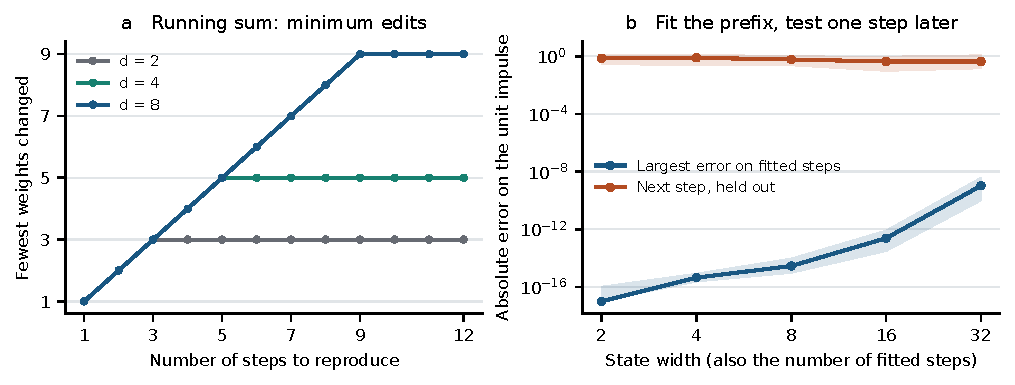
\includegraphics[width=\linewidth]{frontier.pdf}
\caption{A linear recurrent network stores $d$ numbers and returns one fixed state coordinate. At left, choose a number of steps on the horizontal axis. A point gives the fewest individual weights that must change to reproduce all those running sums, for the indicated state width. For example, at width four the cost stops at five edits. These points are exact theoretical values. At right, the horizontal axis is the number of state coordinates. We give each network an input of one followed by zeros and fit its input weights to the first $d$ outputs, all equal to one. The vertical axis gives absolute error on this sequence. Only the right panel aggregates trials: each point is a median across 64 random starts. The bands show the middle 50\% of these runs. The fitted error is the largest absolute error on the prefix. The unseen error is the absolute error on its next coefficient. Values below $10^{-17}$ appear at $10^{-17}$ on the logarithmic axis.}\label{fig:front}
\end{figure}

\section{Can a language model find the predicted edits?}\label{sec:writer}
For a target state $s_t$ at step $t$, choose a multiplier $\lambda$ on its previous value and an input gain $\gamma$. Starting at $s_0=0$, the target rule is $s_t=\lambda s_{t-1}+\gamma x_t$. A running sum has $\lambda=\gamma=1$. In each of six pairs we sent Astra the same initialized network, rule, fixed output coordinate and ordering of entries in the array. One request specified just a prefix and allowed scratch arithmetic. The other specified all horizons and prohibited tools. Each edit was an index and a replacement value. Neither request received test feedback. Table~\ref{tab:astra} reports all six pairs.

\begin{table}[htbp]\centering\small\setlength{\tabcolsep}{3.4pt}
\caption{Paired WSP requests for $s_t=\lambda s_{t-1}+\gamma x_t$, and a BP control given the same editable entries. Here $d$ is state width and $H$ is the short horizon and short edit count. Fit exact counts matching impulse coefficients out of $H$. Next gives the absolute error on coefficient $g_H$, also its single-output RMSE. WSP and BP agree to the three decimal places shown for Next. The last column counts all-horizon WSP edits.}\label{tab:astra}
\begin{tabular}{@{}lrr rr rr rr@{}}\toprule
&&&\multicolumn{2}{c}{Short WSP}&\multicolumn{2}{c}{Short BP}&&All-horizon\\
$(\lambda,\gamma)$&$d$&$H$&Fit exact&Fit RMSE&Fit exact&Fit RMSE&Next&WSP edits\\\midrule
$(1,1)$ & 4 & 2 & 1/2 & $7.85\times10^{-17}$ & 1/2 & $1.57\times10^{-16}$ & 0.156 & 5\\
$(1,1)$ & 5 & 3 & 2/3 & $1.28\times10^{-16}$ & 0/3 & $1.24\times10^{-15}$ & 1.528 & 6\\
$(1,1)$ & 6 & 4 & 2/4 & $3.14\times10^{-16}$ & 0/4 & $2.10\times10^{-14}$ & 0.938 & 7\\
$(-1/2,2)$ & 4 & 2 & 1/2 & $2.21\times10^{-14}$ & 1/2 & $2.20\times10^{-15}$ & 0.630 & 5\\
$(1/2,-1)$ & 5 & 3 & 2/3 & $3.20\times10^{-17}$ & 0/3 & $1.57\times10^{-16}$ & 1.514 & 6\\
$(-1,1/2)$ & 6 & 4 & 2/4 & $6.21\times10^{-17}$ & 0/4 & $9.36\times10^{-15}$ & 0.018 & 7\\
\bottomrule
\end{tabular}\end{table}

All six all-horizon replies set $cA=\lambda c$ and $cb=\gamma$. Substitution into the update proves the target recurrence for every real stream. Each also reproduced all 512 central streams of length eight and all 512 outer streams of length 64 with zero RMSE. The short replies used $H$ edits. Their decimal values met the requested absolute tolerance of $10^{-9}$ on every fitted impulse coefficient, and each missed the next coefficient. The theorem predicts their edit \emph{count} for a real exact fit. The numerical replay measures agreement after rounding.

Two checks separate this result from the behavior of one solver. At width eight, a numerical solve for the input weights on eight impulse coefficients gave a median maximum prefix error of $2.8\times10^{-15}$ and a median next error of $0.588$ over 64 starts (Figure~\ref{fig:front}b). An adaptive gradient method also learned an exact running sum. In a scalar cell with transition weight $a$, input weight $b$ and output equal to its state, a unit gradient step on half the squared final error for the labeled stream $(1)$ sets $b=1$ in real arithmetic. Next choose the input stream $(1,-a)$ and hold its values fixed while differentiating. The output has derivatives $(1,0)$ with respect to $(a,b)$ and its target is $1-a$. A second unit step sets $a=1$. Repeating each update once to accommodate rounding gave exactly $(a,b)=(1,1)$ in 256 of 256 binary64 Xavier draws, with zero RMSE on 512 outer streams per draw.

For a matched numerical control, we disclosed the locations of the WSP edits to BP, froze all other entries and used 800 Adam steps followed by up to 1,000 BFGS iterations. The short control received the same $H$ impulse labels. For the all-horizon control we supplied the first $d+1$ impulse labels, enough to certify an \emph{exact} fit for an order-one target at width $d$. On each of the six outer tests WSP attained 512/512 complete streams with zero RMSE. BP attained 0/512 in each case, with shell RMSE between $1.02\times10^{-13}$ and $1.44\times10^{-11}$. The archive includes all six pairs at full precision.

\section{Proof of Theorem~\ref{th:edit}}\label{app:proof}
We count changes to the \(D=d^2+d\) real entries of the transition matrix \(A\) and input column \(b\) of a width-\(d\) linear recurrent network. The output row \(c\) reads one fixed state coordinate. Renumbering the coordinates preserves edit counts, so take \(c=e_1^\top\), where \(e_1\) is the first standard basis column and \({}^\top\) denotes transpose. Here, the real numbers form the field of coefficients for every calculation in the proof. A unit impulse is input 1 on the first tick and 0 thereafter. Index its desired scalar outputs by \(g_0,g_1,\ldots\) and fix the number \(H\ge1\) of required outputs. For a positive integer \(s\), define the \emph{observation matrix} \(O_s(A)\) by stacking the \(s\) rows \(c,cA,\ldots,cA^{s-1}\). The rank of a matrix is the number of independent columns (equivalently, rows). Its kernel comprises the vectors that it sends to zero. The product of \(O_s(A)\) with \(b\) gives the network's first \(s\) impulse outputs. Write \(g_{0:s-1}=(g_0,\ldots,g_{s-1})^\top\).

Let \(S\) be the forward shift on sequences, so that \((Sg)_i=g_{i+1}\). A monic polynomial has leading coefficient one. For a monic polynomial of degree \(m\), written \(q(z)=z^m+\sum_{j=0}^{m-1}q_jz^j\) in the indeterminate \(z\), set
\[
             (q(S)g)_i=g_{i+m}+\sum_{j=0}^{m-1}q_jg_{i+j}.
\]
Fix the smallest-degree monic polynomial \(p\) for which \(p(S)g=0\) at all indices. Its degree \(r\) is the recurrence order of the nonzero target. We assume \(d\ge r\) until the final step. A \emph{Hankel matrix} is constant on each antidiagonal. The leading \(r\)-by-\(r\) Hankel matrix \(G_r=(g_{i+j})_{0\le i,j<r}\) is invertible. Otherwise a nonzero linear combination of its columns would give a nonzero polynomial of degree less than \(r\) whose filtered sequence has \(r\) initial zeros. Filtering commutes with \(p(S)\), so the recurrence propagates those zeros to every index, contradicting minimality. All columns of the infinite Hankel matrix after the first \(r\) obey the same recurrence, giving overall rank \(r\).

\paragraph{Controlling the characteristic polynomial.}
Call \((c,A)\) \emph{observable} if \(O_d(A)\) has rank \(d\), so the first \(d\) scalar observations distinguish all initial states. Let \(I\) be the \(d\)-by-\(d\) identity, let \(\chi_A(z)=\det(zI-A)\) be the characteristic polynomial, and let \(\mathrm{adj}(M)\) denote the transpose of the cofactor matrix of a square matrix \(M\). For a freely chosen column \(u\in\mathbb R^d\), changing \(A\) to \(A+uc\) changes only column one. The rank-one determinant identity gives
\[
         \chi_{A+uc}(z)-\chi_A(z)=-c\,\mathrm{adj}(zI-A)u .
\]
For observable \((c,A)\), the displayed map from \(u\) to polynomials of degree below \(d\) is a linear bijection. Indeed, if the right side vanishes, so does \(c(zI-A)^{-1}u\) wherever \(zI-A\) is invertible. Its power series in \(1/z\) near infinity has coefficients \(cA^ku\) for integers \(k\ge0\). They all vanish, hence \(O_d(A)u=0\) and \(u=0\). Both spaces have dimension \(d\), proving bijectivity. The new matrix remains observable because \(c(A+uc)^k\) equals \(cA^k\) plus a linear combination of preceding observation rows. Finally, the determinant of \(O_d(A)\) is a polynomial which equals one for the matrix with ones on its first superdiagonal and zeros elsewhere. Its zero set has Lebesgue measure zero. Thus the required observability holds with probability one under the initialization in Theorem~\ref{th:edit}.

\paragraph{Constructing an edit.}
If \(H\le d\), select \(H\) linearly independent columns of \(O_H(A)\). Holding the remaining entries of \(b\) fixed, solve the resulting invertible system for the selected entries of the new input vector \(b'\) to obtain \(O_H(A)b'=g_{0:H-1}\). This takes at most \(H\) edits.

For \(H>d\), put \(k=H-d\). Seek a monic degree-\(d\) polynomial \(q\) such that the first \(k\) terms of \(q(S)g\) vanish. These linear equations in the coefficients of \(q\) are consistent because a monic degree-\(d\) multiple of \(p\) exists. Their \(k\)-by-\(d\) Hankel coefficient matrix has rank \(\min(k,r)\), since it contains the first \(\min(k,r)\) rows of the invertible \(G_r\) and the infinite matrix has rank \(r\). The bijection above lets us impose the equations on \(q=\chi_{A+uc}\) with the same rank in \(u\). Select that many independent columns of this linear system and use just their coordinates of \(u\). Then solve \(O_d(A+uc)b'=g_{0:d-1}\), using at most \(d\) more edits. The Cayley--Hamilton identity says a square matrix satisfies its characteristic polynomial. Consequently the network impulse outputs satisfy the recurrence \(q\), and so agree by induction with the target through the first \(H\) outputs. If \(k\ge r\), the first \(r\) terms of \(q(S)g\) vanish, and the recurrence \(p\) propagates those zeros to all subsequent terms. The total cost is at most \(d+\min(k,r)\).

\paragraph{Bounding the size of the solution set.}
Codimension is the ambient dimension minus the dimension of the subset. We show that the set of \((A,b)\) realizing the prefix has codimension at least \(\min(H,d+r)\), allowing for unobservable realizations. Let \(m=\rank O_d(A)\), and write \(U=\ker O_d(A)\) for the subspace of initial states invisible to the output. Because \(c\ne0\), we have \(1\le m\le d\). The subspace \(U\) has dimension \(d-m\), lies in \(\ker c\), and satisfies \(AU\subseteq U\) by Cayley--Hamilton. The family of possible subspaces \(U\) of this dimension inside the \((d-1)\)-dimensional space \(\ker c\) has dimension \((d-m)(m-1)\). Locally such a subspace is the graph of a linear map between spaces of dimensions \(d-m\) and \(m-1\). For fixed \(U\), the condition \(AU\subseteq U\) forces a block of \(m(d-m)\) entries to vanish in a basis adapted to \(U\). Subtracting the freedom to choose \(U\) leaves codimension at least \(d-m\). Identifying states that differ by an element of \(U\) gives an \(m\)-dimensional quotient space. Denote its induced transition and output by \(\bar A,\bar c\). This quotient is observable.

If \(m\ge H\), the first \(H\) observation rows are independent. Once an observation row belongs to the span of earlier rows, multiplying the relation by \(A\) prevents every subsequent row from increasing that span. Hence the \(H\) impulse equations impose \(H\) constraints on \(b\) for fixed \(A\), as required. If \(m<H\), the first \(m\) impulse equations impose \(m\) independent constraints on \(b\), leaving \(d-m\) free coordinates. Put \(k=H-m\). The other equations require \(q=\chi_{\bar A}\) to satisfy \((q(S)g)_i=0\) for \(0\le i<k\). The coefficient matrix \(B=(g_{i+j})_{0\le i<k,\,0\le j<m}\) has rank \(\rank B\). When consistent, these equations impose that many independent conditions on \(\bar A\). To see this, perturb it by \(\bar u\bar c\) for a quotient-space column \(\bar u\). The characteristic coefficients vary freely by the bijection above, and every such perturbation lifts to a matrix that preserves \(U\). Thus the total codimension for this value of \(m\) is at least \((d-m)+m+\rank B=d+\rank B\).

If \(m\ge r\), then \(\rank B=\min(k,r)\) and \(d+\rank B\ge\min(H,d+r)\). If \(m<r\) and \(k\ge r\), propagation of the initial zeros of \(q(S)g\) would give an annihilating polynomial of degree \(m<r\), contradicting the definition of \(r\). Finally if \(m<r\) and \(k<r\), deleting \(r-k\) rows and \(r-m\) columns of \(G_r\) leaves \(B\), so \(\rank B\ge k+m-r=H-r\). Then \(d+\rank B\ge H\), as required.

\paragraph{From dimension to scalar edits.}
Fix a set of \(s\) coordinates allowed to change. Initial networks which can reach the prefix solution set lie in its sum with the \(s\)-dimensional subspace supported on those coordinates. The solution set is defined by polynomial equations in real parameters. Its sum with this subspace is semialgebraic, meaning that it can be described using finitely many real polynomial equalities and inequalities and Boolean combinations. Its dimension is at most \(D-\min(H,d+r)+s\) because it is the image under addition of a product of that dimension at most. If \(s<\min(H,d+r)\), this is less than \(D\), so the sum has Lebesgue measure zero. There are finitely many choices of coordinates and countably many positive integers \(H\), giving the lower bounds simultaneously with probability one. At \(H=d+r\), the upper and lower constructions give the all-horizon result. For \(d<r\), Cayley--Hamilton would give an annihilating polynomial of degree \(d\), ruling out all-horizon realization. \hfill\(\square\)

\paragraph{Exact arithmetic verification.}
We treated each binary64 Xavier coefficient as its exact rational value. The three test impulse sequences were the constant \(g_n=1\), the Fibonacci numbers \(F_0=0,F_1=1,F_{n+2}=F_{n+1}+F_n\), and the triangular numbers \(T_n=n(n+1)/2\) for nonnegative integers \(n\). We tested five initialization seeds and widths \(1,2,3,4,6,8\) whenever \(d\ge r\). Across 480 cases with \(1\le H\le d+r\), every write changed exactly the predicted number of coordinates. Each of the 405 shorter-horizon writes failed at the next coefficient \(g_H\). At \(H=d+r\), all 75 characteristic polynomials of the edited matrices were divisible by \(p\), and their first 32 impulse coefficients matched directly. Divisibility and agreement on the first \(d\) coefficients then certify every later coefficient.

\section{A comparator that preserves binary64 operands}\label{app:sort}
A comparator takes two inputs and returns their smaller and larger values in that order. Let \(a,b\) be finite binary64 inputs in \([-10,10]\), let \(R(t)=\max(t,0)\) be the rectified linear unit, and take fixed constants \(K=2^{537}\), \(M=10\). Round each displayed operation separately to the nearest binary64 value, choosing the one with even last significand bit at a tie. Gradual underflow retains reduced-precision values below the smallest positive normal number. Numerical equality identifies the two signed zeros.

First extract the positive difference \(r\), amplify it to \(u\), and compute the auxiliary signals \(v,B,S\). Then compute the keep and swap selectors \(k,s\), respectively, in this order:
\[
 r=R(a-b),\quad u=Kr,\quad v=u-R(u-1),\quad B=1-R(1-u),
 \quad S=1-R(1-Kv),
\]
\[
                k=R((1-B)-S),\qquad s=1-k.
\]
For an operand \(x\) and an enable bit \(g\in\{0,1\}\), set
\(G(x,g)=R(x-M(1-g))-R(-x-M(1-g))\). The comparator returns
\((G(a,k)+G(b,s),\,G(a,s)+G(b,k))\), reusing the shifts \(Mk,Ms\).

When \(a\le b\), \(u=B=S=0\) and \(k=1\). When \(a>b\), the rounded positive difference is at least the smallest representable positive value \(2^{-1074}\). For \(0<u\le1\), \(v=u\) and \(Kv\ge1\), hence \(S=1\). For \(u\ge1\), \(B=1\). In that case the rounded value of \(u-1\) lies between \(u-2\) and \(u\), since \(u\) itself is representable and is one unit of absolute distance from the exact difference. Therefore \(0\le v\le2\), which also shows that the product \(Kv\) remains finite. Both \(B,S\) lie in \([0,1]\) and at least one equals one, so \(k=0\). For \(g=1\) the gate \(G\) returns the original operand, while for \(g=0\) both rectifiers vanish. Composition along a sorting schedule therefore preserves all numerical operands. The stored comparator contains 43 edge weights and seven biases, with Xavier initialization for the weights and zero initialization for the biases.

\section{Scalar construction and size sweeps}\label{app:square}
For a real input \(x\in[-16,16]\), set \(t=|x|/16\). Define the tent map \(T(t)=2t-4R(t-1/2)\) on \([0,1]\), where \(R(t)=\max(t,0)\). For a positive integer refinement depth \(m\), let \(T^{\circ i}\) denote \(i\) successive applications of \(T\). The depth-\(m\) square interpolant is
\[
               256\left[t-\sum_{i=1}^m4^{-i}T^{\circ i}(t)\right].
\]
At each refinement, the added term corrects the midpoint error of the preceding linear interpolant on intervals with endpoints at multiples of a power of two. The maximum absolute error of the resulting interpolant on \([-16,16]\) in real arithmetic is \(64\cdot4^{-m}\). The compact model starts at hidden width two, uses width three in its remaining layers, and has an affine output and \(12m+5\) parameter slots.

For the compensated version let \(q\) denote the running unscaled sum and \(u\) its next term to subtract. Compute the rounded difference \(s=q-u\), then \(d=q-s\), then \(e=d-u\), using the compensated subtraction transform \cite{dekker1971}. Accumulate \(R(e)\) and \(R(-e)\) separately. Add their difference to the last \(q\) before scaling the output. Copying nonnegative intermediate results through rectifiers implements the stated arithmetic with maximum hidden width six and \(203m+35\) slots. In exact real arithmetic \(e=0\). Setting only the two weights that read the error accumulators to zero tests the numerical contribution of the compensation.

To construct difficult shell inputs, express a positive normal input as \(x=N\,2^{e-52}\), where the integer exponent \(e\) places \(x\) in the interval \([2^e,2^{e+1})\) and \(N\) is its 53-bit integer significand. The low bits of \(N^2\) determine which side of a rounding midpoint contains \(x^2\). Let \(k\in\{52,53\}\) count the discarded bits and take \(j\in\{7,15,\ldots,255\}\). Find integers satisfying \(N^2\equiv2^{k-1}-j\pmod{2^k}\) by extending the low bits one at a time. Retain significands with the specified discard count and shell magnitude, then include both signs. This gives 304 inputs from 152 magnitudes. Networks with 35, 48 and 55 refinements match respectively \(0,40,304\) of these inputs. All three match all 131,072 fresh uniform shell inputs. On 501 small powers \(x=2^n\), \(-500\le n\le0\), the same networks match 32, 45 and 52 inputs. The first affine segment near zero gives large relative errors despite small absolute errors.

\section{Historical controls with an extrapolation-first WSP prompt}\label{app:historical}
This preliminary study used an extrapolation-first prompt and included affine arithmetic and memoryless sum controls. All counts in this appendix refer to that earlier design. A network's \emph{architecture} specifies which operations it applies and where coefficients can enter. For the scalar tests, an \emph{affine} function multiplies input values by fixed coefficients, sums them and adds a constant. A \emph{rectified linear unit} (ReLU) is the scalar function $R(u)=\max(0,u)$ of a real input $u$. Let $w$ count the hidden units, let $a,b$ denote the slope and offset of a direct input-to-output path (a \emph{skip}), and give hidden unit $j$ input slope $u_j$, offset $v_j$ and output weight $c_j$. The shallow network computes
\[
                 f(x)=ax+b+\sum_{j=1}^{w}c_j R(u_jx+v_j).
\]
Each hidden unit contributes a \emph{hinge}, a possible change of slope at its zero crossing (a \emph{knot}). This architecture has $3w+2$ scalar slots.

We tested the square, sine in radians, positive self-power $x^x$, hyperbolic tangent $\tanh x=(e^{2x}-1)/(e^{2x}+1)$ with $e$ the base of the natural logarithm, addition, subtraction, running sum, sorting four inputs in ascending order, Fibonacci numbers, and triangular numbers. At integer index $n\ge0$, Fibonacci numbers start at $F_0=0,F_1=1$ and obey $F_{n+2}=F_{n+1}+F_n$. The triangular number is $T_n=n(n+1)/2$. Self-power uses positive real inputs. Appendix~\ref{app:signed} handles the separate negative-integer extension.

For each task and each of three random starts, two independent Astra requests saw the same three architectures, weights, deployment envelope and labeled examples. One request supplied \emph{the formula and examples}. The other supplied \emph{examples only}, omitting the task name and rule. Each request returned three complete arrays. This gives 60 calls and 180 WSP arrays. All 180 could be executed. The three arrays from a single call are dependent. This protocol allows a complete overwrite. Only Section~\ref{sec:front} minimizes edits. For each of the 90 task, size and start combinations we also fit all slots using BP with 800 Adam updates followed by up to 1,000 BFGS iterations. Each solver saw 12 central examples except on the integer-sequence tasks, which used indices 0 through 8. WSP was asked to prioritize the \emph{largest} scaled error. BP minimized half the \emph{mean squared} scaled error. Architectures, examples and initial arrays were paired. Objectives, prior knowledge and computational budgets differed.

\begin{table}[htbp]\centering\small\setlength{\tabcolsep}{3.5pt}
\caption{Held-out outer predictions on the same networks. Each method has an exact-match percentage and a raw root mean squared error (RMSE). Entries are medians over three starts. Formula and examples and examples only are the two weight-space programming (WSP) conditions. The backpropagation condition receives examples only. Scalar scores use 2,048 inputs per available shell side. Addition, subtraction, running sum and sorting each use 2,048 inputs or lists. A list must match at every position. Each Fibonacci or triangular score uses the 32 indices from 33 through 64 of one trajectory.}\label{tab:paired}
\begin{tabular}{@{}lr rr rr rr@{}}\toprule
&&\multicolumn{2}{c}{\textbf{WSP}}&\multicolumn{2}{c}{\textbf{WSP}}&\multicolumn{2}{c}{\textbf{Backpropagation}}\\
&&\multicolumn{2}{c}{Formula and examples}&\multicolumn{2}{c}{Examples only}&\multicolumn{2}{c}{Examples only}\\
\cmidrule(lr){3-4}\cmidrule(lr){5-6}\cmidrule(l){7-8}
Target & Slots & Exact \% & RMSE & Exact \% & RMSE & Exact \% & RMSE\\\midrule
$x^2$ & 50 & 0.0 & 0.644 & 0.0 & 0.633 & 0.0 & 29.5\\
$\sin x$ & 50 & 0.0 & 0.0335 & 0.0 & 0.0324 & 0.0 & 2.46\\
$x^x$, positive & 50 & 0.0 & $1.3\times 10^{8}$ & 0.0 & $1.3\times 10^{8}$ & 0.0 & $1.6\times 10^{9}$\\
$\tanh x$ & 50 & 0.0 & 0.00154 & 0.0 & 0.0015 & 0.0 & 0.52\\
Addition & 2 & 100.0 & 0 & 100.0 & 0 & 27.2 & $2.3\times 10^{-15}$\\
Subtraction & 2 & 100.0 & 0 & 100.0 & 0 & 1.3 & $4.7\times 10^{-15}$\\
Running sum & 3 & 100.0 & 0 & 100.0 & 0 & 0.0 & $2.3\times 10^{-14}$\\
Sort four & 40 & 53.5 & $5.2\times 10^{-16}$ & 53.6 & $5.0\times 10^{-16}$ & 0.6 & 5.95\\
Fibonacci & 8 & 100.0 & 0 & 100.0 & 0 & 0.0 & 0.269\\
Triangular & 15 & 100.0 & 0 & 100.0 & 0 & 0.0 & $2.1\times 10^{-8}$\\
\bottomrule
\end{tabular}
\end{table}

For this preliminary study, Table~\ref{tab:paired} uses the largest tested shallow scalar width (16 hinges) and the smallest tested size known to suffice over the reals for each algorithmic task. Both WSP conditions achieved perfect outer scores on addition, subtraction, running sum, Fibonacci and triangular numbers at those sizes. The examples-only condition still exposed a task-specific graph and recognizable labels. At width 16 all four smooth targets had zero exact outer matches for either WSP condition and for BP. On square, however, examples-only WSP had RMSE 0.633 versus 29.5 for BP. For sorting, formula-and-examples WSP matched only 53.5\% of complete vectors, but its RMSE was $5.2\times10^{-16}$. With a gradient fit the corresponding values were 0.6\% and 5.95. Appendix~\ref{app:additional} retains the scale-adjusted results, which reveal a different aspect of errors on rapidly growing $x^x$.

\paragraph{How close was each fit to the best training loss?}
The training loss is half the mean of $[(\hat y_i-y_i)/\max(1,|y_i|)]^2$ over observed scalar outputs. For the 12 one-hinge settings (four smooth functions and three starts), we computed the globally smallest \emph{real-arithmetic} loss on the stored binary64 labels by enumerating all intervals in which the knot can lie. For a second gradient-based optimizer, \emph{trust-region least squares} fits a local linear approximation of all output errors and restricts the update to a neighborhood where that approximation is useful. We applied it both at the original weights and after WSP.

Using an absolute training-loss gap of $10^{-10}$ to the certified optimum, Adam succeeded in 0/12 settings, Adam followed by BFGS in 1/12, and trust-region least squares from the same Xavier weights in 5/12. Starting least squares from examples-only WSP raised that to 9/12. Among the 90 settings, least squares from Xavier obtained six completely exact outer sets, all on addition or subtraction. In contrast, both WSP conditions obtained 30/90. The stronger optimizer improved a central objective without guaranteeing transfer. Refining the formula-and-examples WSP arrays reduced training loss materially in 54 settings. It improved outer mean scaled absolute error in seven and worsened it in 47. Figure~\ref{fig:optim} gives the paired counts. Appendix~\ref{app:optimizer} reports the per-task RMSE comparisons, solver budgets and optimality argument. Appendix~\ref{app:convex} repeats the comparison with hidden units frozen so that the output weights admit an exact least-squares characterization.

\begin{figure}[htbp]
\centering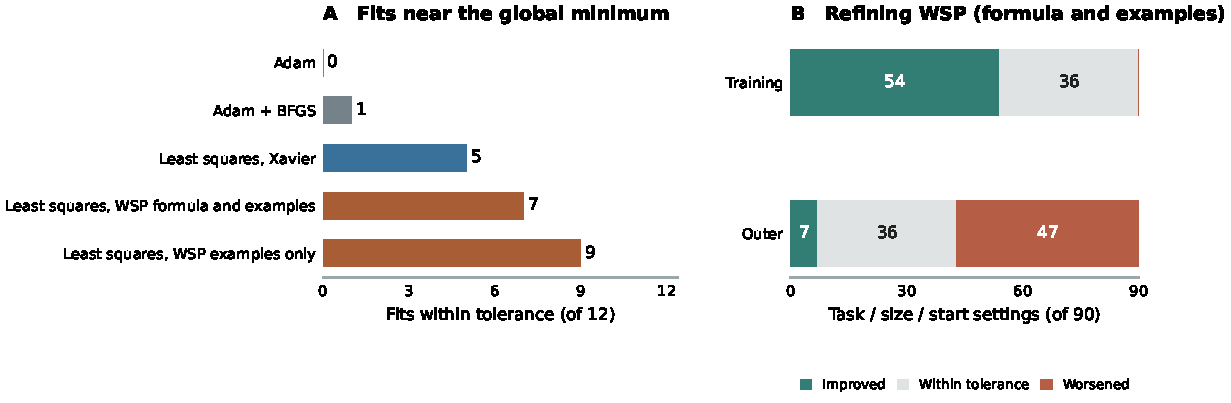
\includegraphics[width=\linewidth]{optimizer.pdf}
\caption{Optimization of the central labels and transfer to the outer shell. Panel a counts fits whose observed loss lies within $10^{-10}$ of the certified real minimum across 12 one-hinge settings. Panel b starts from formula-and-examples WSP and refines each of 90 arrays by least squares. Lower is better. An absolute change of at most $10^{-10}$ is classified as within tolerance. Training uses half the mean squared scaled error, and outer evaluation here uses mean scaled absolute error. Table~\ref{tab:paired} gives raw RMSE in output units.}\label{fig:optim}
\end{figure}

\paragraph{How did conventional recurrent networks fare?}
A hyperbolic-tangent recurrent cell applies $\tanh$ to its updated state. A gated recurrent unit (GRU) uses gates, numbers between zero and one computed from the current input and previous state, to regulate state retention and updating. We trained both on running sums, Fibonacci and triangular recurrences with two variable starting values, and list sorting in which a shared cell first reads a list and then emits its sorted elements. All 102 task, cell, width and initialization settings were fit at two budgets. None of the resulting 204 fits returned a complete exact example on any of the four held-out sets (central, changed magnitude, changed length, or both). A different one-state $\tanh$ cell, with its hidden scale fixed to $2^{-40}$ and two weights learned from ordinary central labels, learned the exact running sum in three of five starts. Each successful start matched all 1,024 outer length-32 streams, with zero RMSE. Appendix~\ref{app:passive-rnn} gives the update equations, unscaled errors and the separate results for the WSP state scaling.

\section{Additional value and sequence extrapolation controls}\label{app:additional}
The extrapolation-first experiment in Appendix~\ref{app:historical} reports error in target units. Table~\ref{tab:scaled} gives that experiment's scaled absolute errors so that large targets, such as positive self-power near ten, can also be interpreted on a relative scale.

\begin{table}[htbp]\centering\small
\caption{The same ten architectures and outer inputs as Table~\ref{tab:paired}. Entries are mean absolute errors after dividing each error by the larger of one and the absolute reference value, followed by the median over three starts.}\label{tab:scaled}
\begin{tabular}{@{}lrrr@{}}\toprule
&\multicolumn{2}{c}{Weight-space programming (WSP)}&Backpropagation\\
Target & Formula and examples & Examples only & Examples only\\\midrule
Square & 0.0113 & 0.0112 & 0.419\\
Sine & 0.0289 & 0.0279 & 1.83\\
Positive self-power & 0.0774 & 0.0804 & 0.979\\
Hyperbolic tangent & 0.00133 & 0.00132 & 0.367\\
Addition & 0 & 0 & $3.38\times10^{-16}$\\
Subtraction & 0 & 0 & $1.05\times10^{-15}$\\
Running sum & 0 & 0 & $2.46\times10^{-15}$\\
Sort four & $3.91\times10^{-17}$ & $3.72\times10^{-17}$ & 0.776\\
Fibonacci & 0 & 0 & $8.43\times10^{-14}$\\
Triangular & 0 & 0 & $1.06\times10^{-11}$\\
\bottomrule
\end{tabular}\end{table}

\paragraph{Analytic choices of hinge positions.}
For the earlier scalar study, two WSP constructions choose knot locations from the known target expression. Central WSP uses only knots in the central interval. Full-envelope WSP uses formula values outside it. Both use 63 hinges plus a direct affine path (191 slots). The BP comparator sees central labels and uses Adam followed by limited-memory BFGS, which estimates curvature from a short history of changes in weights and gradients. Table~\ref{tab:scalar} shows mean absolute error (MAE), the average of $|\hat y_i-y_i|$, alongside RMSE.

\begin{table}[htbp]\centering\small\setlength{\tabcolsep}{4pt}
\caption{Outer errors for the analytic WSP and gradient controls. Mean absolute error (MAE) is the average absolute prediction error. All methods had 0\% exact on all four tasks at this width. Evaluation uses 4,096 samples per available shell side. BP columns give medians over three starts. The two signed sides are pooled before computing RMSE.}\label{tab:scalar}
\begin{tabular}{@{}l rr rr rr@{}}\toprule
&\multicolumn{2}{c}{Central WSP}&\multicolumn{2}{c}{Full-envelope WSP}&\multicolumn{2}{c}{Backpropagation}\\
Target&MAE&RMSE&MAE&RMSE&MAE&RMSE\\\midrule
Square & 16.6 & 22.2 & 0.00737 & 0.00829 & 16.9 & 22.6\\
Sine & 3.26 & 4.08 & 0.00486 & 0.00602 & 3.26 & 4.07\\
Hyperbolic tangent & 0.0332 & 0.0395 & $1.12\times10^{-5}$ & $3.22\times10^{-5}$ & 0.0919 & 0.109\\
Positive self-power & $4.32\times10^{8}$ & $1.46\times10^{9}$ & $9.55\times10^{6}$ & $3.54\times10^{7}$ & $4.32\times10^{8}$ & $1.46\times10^{9}$\\
\bottomrule
\end{tabular}\end{table}

A WSP sine construction first folds the input using its known period and reflection symmetry, then fits its final spline to 1,024 central labels. Outer MAE was $4.75\times10^{-5}$ at 211 slots. For self-power, reallocating knots and centering the error using the formula reduced maximum relative shell error to 1.01\%. A single native hyperbolic-tangent activation between identity maps matches the same library function by construction. Ten Gauss--Newton steps, which approximate nonlinear least squares by successive linear least-squares updates, gave 100\% shell accuracy from all three starts and 89.1--93.2\% inner accuracy. A two-weight affine model learned addition and subtraction exactly in three starts with 64 full-batch gradient updates. Per-split errors for these variants are in the accompanying data.

\paragraph{Fixed sequence interfaces.}
Table~\ref{tab:seq} compares WSP and BP on the original multistep tasks. In an autonomous linear network, a column $v$ reads out starting state $h_0$ after $n$ transitions as $v^\top A^n h_0$. Its state width must be at least the recurrence order. Fibonacci and triangular numbers require widths two and three, respectively, in this homogeneous model (no additive state offset). A one-state running sum uses unit input, transition and readout weights. Setting the scalar input weight to one and adjusting the readout to preserve their product leaves the real input--output function unchanged. On the same 256 training streams this parameterization yielded exact weights in four of five fresh starts, or three of five starts matched for initial function. Each successful run matched all tested streams at both lengths.

\begin{table}[htbp]\centering\small
\caption{Exact rate and raw root mean squared error (RMSE) for WSP and backpropagation. Sums use 2,048 central length-eight streams and 2,048 outer length-32 streams. Sorting uses 2,048 four-item lists per split. These two exact rates require complete outputs. Fibonacci and triangular rates count indices on one trajectory, the nine \emph{fitted} indices 0--8 versus the 32 \emph{held-out} indices 33--64. Values are medians over five starts.}\label{tab:seq}
\begin{tabular}{@{}lrl r r r r@{}}\toprule
&&&\multicolumn{2}{c}{WSP}&\multicolumn{2}{c}{Backpropagation}\\
Target & Slots & Split & Exact \% & RMSE & Exact \% & RMSE\\\midrule
Running sum & 3 & Central & 100.00 & 0 & 0.93 & $5.42\times10^{-16}$\\
Running sum & 3 & Outer & 100.00 & 0 & 0.00 & $6.94\times10^{-15}$\\
Fibonacci & 8 & Central & 100.00 & 0 & 11.11 & $5.67\times10^{-15}$\\
Fibonacci & 8 & Outer & 100.00 & 0 & 0.00 & 0.0531\\
Triangular & 15 & Central & 100.00 & 0 & 0.00 & $2.36\times10^{-14}$\\
Triangular & 15 & Outer & 100.00 & 0 & 0.00 & $1.02\times10^{-8}$\\
Sort four & 15 & Central & 65.14 & $1.21\times10^{-16}$ & 0.00 & 1.22\\
Sort four & 15 & Outer & 53.96 & $5.12\times10^{-16}$ & 0.00 & 4.94\\
\bottomrule
\end{tabular}\end{table}

The sorter in this table fixes the order of five pair comparisons and stores three adjustable gains per comparison (15 slots). Tying these five sets uses three stored gains. The 40-slot sorter in the main comparison instead learns eight coefficients per step on four wires, including which wires to combine. The operand-preserving comparator stores 50 coefficients in one block shared across all comparisons. From central labels, a search over 9,331 schedules of up to five pair comparisons found 12 shortest sorting schedules. A rational linear solve recovered Fibonacci and triangular recurrences from nine central labels. These controls supply mathematical structure to the solver.

\section{First-response WSP pilot across nine tasks}\label{app:literal}
We made nine independent requests, one per task listed below, beyond the twelve recurrence requests of Appendix~\ref{sec:writer}. Each prompt gave Astra the formula, required domain, architecture and exact initialized weights, and requested one complete vector of replacement weights. The model could perform scratch arithmetic. It received no test feedback. For square, sine and positive self-power, the graph used a seven-hinge hidden layer and a direct affine input--output connection (23 stored scalars). Hyperbolic tangent used the native activation between two affine transformations. Addition and subtraction had two coefficients each. The homogeneous recurrent networks for Fibonacci and triangular numbers used widths two and three respectively. The sorting graph used five prespecified pairs of wires and reused three scalar coefficients on every pair. Untying those coefficients at each comparison gives the 15-slot sorter in Table~\ref{tab:seq}. Five freely routed four-wire residual blocks use 40 slots (Appendix~\ref{app:matched}). The 50-slot sorter stores one operand-preserving block for repeated use (Appendix~\ref{app:sort}).

\paragraph{Scoring the nine WSP responses.}
For continuous inputs, the central and outer tests each contained 4,096 examples. Outer input signs were sampled within this total whenever both signs belonged to the task. Number-sequence rows score the nine individual central indices \(0,\ldots,8\) and 56 later indices \(9,\ldots,64\) from one sequence. Four-item sorting requires all four entries of a vector for an exact match. RMSE includes every scalar output on the split. Scaled absolute error for prediction \(\hat y\) and label \(y\) is \(|\hat y-y|/\max(1,|y|)\). The binary64 reference is the specified NumPy operation, or the integer valued sequence. All entries below are for one response per task. The matched WSP/BP comparison is in Section~\ref{sec:matched}.

\begin{center}
\begin{minipage}{\linewidth}
\centering
\makeatletter\def\@captype{table}\makeatother
\caption{First WSP response on each of nine tasks. Exact percentages and raw RMSE use the same central and outer observations. Addition and subtraction have separate, identical scores.}\label{tab:pilot}
\small\setlength{\tabcolsep}{3.5pt}
\begin{tabular}{@{}lrrrrr@{}}\toprule
& & \multicolumn{2}{c}{Exact (\%)} & \multicolumn{2}{c}{Raw RMSE}\\
Target & Slots & Central & Outer & Central & Outer\\\midrule
\(x^2\) & 23 & 0 & 0 & .514 & .547\\
\(\sin x\) & 23 & 0 & 0 & .0985 & .0934\\
\(x^x,\ x>0\) & 23 & 0 & 0 & 2.65 & \(5.24\times 10^8\)\\
\(\tanh x\) & 4 & 100 & 100 & 0 & 0\\
Addition and subtraction (each) & 2 & 100 & 100 & 0 & 0\\
Fibonacci & 8 & 100 & 100 & 0 & 0\\
Triangular & 15 & 100 & 100 & 0 & 0\\
Sort four & 3 & 64.33 & 55.13 & \(1.18\times10^{-16}\) & \(4.91\times10^{-16}\)\\\bottomrule
\end{tabular}
\end{minipage}
\end{center}
The square response used skip slope \(-17.5\), intercept \(-75.78125\), unit hinge input slopes, knots at \(-7.5,-5,-2.5,0,2.5,5,7.5\) and slope increases of 5. This shifted equal-spacing spline attains the width-seven uniform-error optimum \(50/64=0.78125\) over the real interval. The sine response had maximum absolute error 0.13822, positive self-power had maximum scaled error 0.48922, and the maximum coordinate error of the sorter was \(3.55\times10^{-15}\). The exact arithmetic weights were \((1,1)\) for addition and \((1,-1)\) for subtraction. The tanh response used identity maps around the native activation.

For the \emph{initial suite}, the archive contains all 21 prompts and replies. Metadata record the requested service alias \texttt{gpt-6-astra}, reasoning effort setting, completed event types and token counts. Requests used fresh isolated chats. The provider may change the deployment behind this alias. Archived arrays can be replayed independently in the specified numerical environment.

\section{Experimental detail and reproducibility}
\label{app:exp}
\paragraph{Hardware and arithmetic.} The initial suite used binary64 arithmetic on an Apple M5 central processing unit. For the initial scalar experiments, the environment used Python 3.13.12. The main sequence, frontier and archive scoring environments used Python 3.12.12. Both used NumPy 2.5.4 and the macOS Accelerate implementation of the Basic Linear Algebra Subprograms (BLAS), with SciPy 1.18.1 for optimization. Exact rational computations, which retain integer numerators and denominators, use Python's \texttt{Fraction}. Stream sums use successive rounded additions in temporal order. In this suite the transcendental labels are the platform NumPy results. Tests compare to that implementation. Correct rounding of transcendental functions is a separate question. Re-running with a different BLAS or math library can affect last bits and optimizer paths.

\paragraph{Initialization and budgets.} Let \(n_{\rm in}\) and \(n_{\rm out}\) be the input and output coordinate counts of a layer (its fan-in and fan-out). Xavier initialization draws each weight uniformly between the negative and positive values of \(\sqrt{6/(n_{\rm in}+n_{\rm out})}\). Biases start at zero. Nominal tensor slots include zeros. We count distinct stored trainable coefficients separately from unrolled uses and count edits separately from either. Scalar widths are \(0,1,3,7,15,31,63\). Compact tent depths are \(1,4,8,12,16,20,24,27,30\). The compensated depths are \(16,24,27,30,35,40,48,55\). In the local and full-envelope WSP spline controls, all coefficients were overwritten using the specified formula. Let \(t_j\) be an interior knot and \(s_{j-1},s_j\) the slopes of the adjacent secants. The corresponding hinge has input weight \(w_j=1\), bias \(c_j=-t_j\) and output weight \(v_j=s_j-s_{j-1}\). A linear skip carries the leftmost secant. No samples from the outer test arrays enter training or checkpoint selection.

Adam, the adaptive moment estimation optimizer, updates weights using running estimates of the first and second moments of the training gradients. The quasi-Newton optimizer BFGS is named for Broyden, Fletcher, Goldfarb and Shanno. Its limited-memory version with support for bounds is L-BFGS-B. A minibatch is a sampled subset of training examples used for one update. The shallow scalar gradient runs use three seeds (11, 22, 33), 1,024 in-range training points, 500 minibatch Adam updates of size 64 with learning rate \(0.01\), then at most 250 full-batch L-BFGS-B iterations. We retain the endpoint with smaller training mean squared error (MSE), the mean of squared scalar prediction errors. The compact deep square runs use 300 Adam updates and at most 100 L-BFGS-B iterations. Inner scoring uses 4,096 points and outer scoring uses 4,096 per sign where defined. Tanh polishing uses ten least-squares solves with the full analytic Jacobian. For the affine control let \(X\) collect the training input rows and \(N\) count the rows. The gradient step size is the reciprocal of the largest eigenvalue of \(X^\top X/N\). Phase folding uses six rectifiers to implement the piecewise-linear triangular wave \(\arcsin(\sin x)\), where \(\arcsin\) is the inverse sine taking values in \([-\pi/2,\pi/2]\), on the declared envelope. Its readout uses a least-squares fit on folded central examples. Identical-shape end-to-end training yields median shell mean absolute error (MAE) 3.169.

Sequence sweeps use widths \(1,2,4\) for rolling sum and \(1,2,3,4\) for the two autonomous sequences. Slots total \(d^2+2d\) including a learned readout. The ordinary four-item sorter sweeps three, four, and five untied gates and an additional full tied model. Training uses 256 inner streams of length eight or 256 four-item sort examples. Test sets use 2,048 examples per split. The autonomous tasks use one integer trajectory, first nine labels for training. Each of the 15 configurations uses five independent Xavier seeds, 800 full-batch Adam updates at 0.02 with gradient-norm cap 5, then BFGS up to 1,000 iterations. Objective is half mean squared residual. For a target sequence value \(g_n\) at index \(n\), integer-sequence residuals are divided by \(\max(1,|g_n|)\) before squaring. We checked reverse-mode gradients, obtained by propagating output derivatives backwards through the graph, against centered finite differences obtained from small positive and negative parameter perturbations. We report medians across seeds and retain each seed's scores, convergence status and final tensors. With shared three-gain sorting, individual BP fits range from zero to \(46.39\%\) whole-shell equality. With \(\epsilon=2^{-52}\) denoting the gap above 1 in binary64 and \(y\) the reference coordinate, the best fit passes the whole-vector \(8\epsilon\max(1,|y|)\) test on every four-item example.

\paragraph{Activation and magnitude controls.} Writing \(x_t\) for the current input, \(h_t\) for the scalar state after tick \(t\) and \(y_t\) for its output, a conventional one-state tanh RNN \(h_t=\tanh(h_{t-1}+2^{-40}x_t)\), \(y_t=2^{40}h_t\), reproduced every measured held-out prefix on the same binary64 tests. For the small arguments encountered on these samples, the library tanh returns its input value. The output is bounded, and scaling subnormal values can erase inputs outside the tested conditions. The matched five-start gradient model had median outer length-32 RMSE 0.452 and zero whole-stream accuracy at the median. The ordinary sorting control with gains fixed to one recovers every lattice vector because differences and outputs stay representable. The 50-weight selection comparator is trained on the same sorting task in a separate matched-architecture run. Its median outer RMSE is 4.35, compared with zero for the WSP comparator on that set. For the full-width, depth-48 square we tested the effect of setting the compensation readout coefficients to zero. The associated gradient experiment trained the compact deep family.

\paragraph{Reproducible outputs.} The accompanying code includes raw per-split tables, fixed generators and seed-level results, exact-rational validations, the individual Astra responses and functions to apply them. A replay of the rational weights obtained by setting the transition matrix characteristic polynomial after rounding them to binary64 produced 32/32 exactly matching impulse values in 15 of 75 cases. These were 14/30 for prefix sum, 1/25 for Fibonacci and 0/20 for triangular numbers under fixed-order separate multiply/add. This is specific to that construction and its reduction order. The isolated-row implementation exploits a different coordinate support. All observations in this initial suite are synthetic. The later transcendental studies also use published difficult-input corpora.


\paragraph{Width sweep of shallow scalar networks.}
For each hidden width, the first table gives mean absolute error on the outer range. Its WSP network uses uniform knots and formula values throughout the deployment envelope. BP uses central data only and its cell is the median of three independently initialized fits. A stored slot is one scalar coefficient, including a coefficient set to zero. The number of slots is three times the hinge count plus two.
\begin{center}
\begin{minipage}{\linewidth}
\centering
\makeatletter\def\@captype{table}\makeatother
\caption{Mean absolute error (MAE) on the outer shell for shallow networks of increasing hidden width. WSP has access to the formula throughout the envelope. BP uses central labels.}\label{tab:initial_mae}
\small
\begin{tabular}{@{}rr|rr|rr|rr@{}}\toprule
& & \multicolumn{2}{c|}{\(x^2\)} & \multicolumn{2}{c|}{\(\sin x\)} & \multicolumn{2}{c}{\(x^x\)}\\
Hinges & Slots & WSP & BP & WSP & BP & WSP & BP \\\midrule
0  & 2   & 23.3 & 43.0 & 0.692 & 2.23 & \(6.08\times 10^9\) & \(4.32\times 10^8\)\\
1  & 5   & 8.67 & 28.1 & 0.692 & 2.60 & \(3.15\times 10^9\) & \(4.32\times 10^8\)\\
3  & 11  & 1.82 & 21.9 & 0.755 & 2.21 & \(1.37\times 10^9\) & \(4.32\times 10^8\)\\
7  & 23  & 0.485 & 20.8 & 0.212 & 2.75 & \(4.92\times 10^8\) & \(4.32\times 10^8\)\\
15 & 47  & 0.121 & 18.2 & 0.0726 & 3.05 & \(1.42\times 10^8\) & \(4.32\times 10^8\)\\
31 & 95  & 0.0296 & 16.4 & 0.0195 & 3.30 & \(3.69\times 10^7\) & \(4.32\times 10^8\)\\
63 & 191 & 0.00737 & 16.9 & 0.00486 & 3.26 & \(9.55\times 10^6\) & \(4.32\times 10^8\)\\\bottomrule
\end{tabular}
\end{minipage}
\end{center}

The second table reports raw RMSE in the same target units on the same split, pooling scalar observations from the two shell sides before computing the seed median. Positive self-power uses the positive side alone. The closely spaced WSP knots at larger widths reduce absolute errors. The positive self-power target reaches approximately \(10^{10}\) in this shell.
\begin{center}
\begin{minipage}{\linewidth}
\centering
\makeatletter\def\@captype{table}\makeatother
\caption{Root mean squared error (RMSE) for the same shallow networks and outer draws. WSP uses full-envelope knots, and BP is the median of three fits.}\label{tab:initial_rmse}
\scriptsize\setlength{\tabcolsep}{2.8pt}
\begin{tabular}{@{}rr|rr|rr|rr|rr@{}}\toprule
 & & \multicolumn{2}{c|}{Square} & \multicolumn{2}{c|}{Sine} & \multicolumn{2}{c|}{Self-power} & \multicolumn{2}{c}{Tanh}\\
Hinges & Slots & WSP & BP & WSP & BP & WSP & BP & WSP & BP\\\midrule
0 & 2 & $26.7$ & $50.5$ & $0.817$ & $2.31$ & $6.34\times 10^{9}$ & $1.46\times 10^{9}$ & $0.404$ & $2.13$\\
1 & 5 & $9.41$ & $34.8$ & $0.817$ & $3$ & $4.24\times 10^{9}$ & $1.46\times 10^{9}$ & $0.404$ & $1.68$\\
3 & 11 & $2.05$ & $28.1$ & $0.97$ & $2.82$ & $2.56\times 10^{9}$ & $1.46\times 10^{9}$ & $0.122$ & $0.336$\\
7 & 23 & $0.54$ & $26.9$ & $0.258$ & $3.47$ & $1.26\times 10^{9}$ & $1.46\times 10^{9}$ & $0.00249$ & $0.174$\\
15 & 47 & $0.135$ & $24$ & $0.0933$ & $3.83$ & $4.60\times 10^{8}$ & $1.46\times 10^{9}$ & $8.06\times 10^{-4}$ & $0.14$\\
31 & 95 & $0.0332$ & $22$ & $0.0239$ & $4.13$ & $1.33\times 10^{8}$ & $1.46\times 10^{9}$ & $1.14\times 10^{-4}$ & $0.156$\\
63 & 191 & $0.00829$ & $22.6$ & $0.00602$ & $4.07$ & $3.54\times 10^{7}$ & $1.46\times 10^{9}$ & $3.22\times 10^{-5}$ & $0.109$\\
\bottomrule

\end{tabular}
\end{minipage}
\end{center}

\section{Signed indices and the negative shell}\label{app:signed}
The central integer set is \(\{-3,\ldots,3\}\). The outer sets are \(\{-10,\ldots,-4\}\) and \(\{4,\ldots,10\}\). For negative binary64 inputs, each noninteger has a reduced rational representation with an even denominator. Raising a negative base to that exponent has no conventional real value. On the 21 integers from \(-10\) to 10, by contrast, \(n^n\) is rational, with \(0^0=1\) by continuity from the positive side. NumPy's result equals the once-rounded rational reference at every index. A 572-slot rectifier lookup uses one triangular hat per integer. A hat equals one at its own integer and zero at all other integers. Setting its readout coefficient to the target value matched all seven central integers, seven negative-shell integers and seven positive-shell integers. Among the linear output weights that fit the seven central labels, the solution of smallest Euclidean norm in the same feature map missed all 14 shell integers. On the seven negative and seven positive outer integers, WSP gave RMSE zero for both signs. BP from a Xavier readout on the same frozen hats gave outer RMSE .314 and \(3.78\times10^9\), respectively. The minimum-norm readout instead gave .00148 and \(3.78\times10^9\). Each central-only fit missed every outer index. The full WSP lookup stores the specified answers.

For integer index \(n\), let \(F_n\) denote the Fibonacci value and \(T_n=n(n+1)/2\) the triangular value. For \(n>0\) the signed Fibonacci convention is \(F_{-n}=(-1)^{n+1}F_n\). The input consists of \(|n|\) unit ticks and a supplied sign selecting the forward or inverse transition. Each model stores forward and inverse transition matrices, an initial state, and a readout. The width-two Fibonacci and width-three triangular models therefore use 12 and 24 scalar slots. A direct write and a rational recurrence inferred from only \(n=-3,\ldots,3\) both matched 7/7 central, 7/7 negative-shell, and 7/7 positive-shell labels, compared with independent integer formulas. In teacher-forced training, the true preceding values are fed into each one-step update. A gradient fit on those same central windows and the supplied shift structure achieved 14/14 shell accuracy in one of five starts for each task. WSP gave zero RMSE for each task and each sign. The median BP RMSE over five starts on the negative and positive shells, respectively, was \(3.93\times10^{-14}\) and \(3.49\times10^{-14}\) for Fibonacci and \(7.21\times10^{-14}\) and \(1.33\times10^{-13}\) for triangular numbers.

\paragraph{Observed sizes versus certified minima.}
The minimum state widths are one for the driven linear accumulator and two and three for the homogeneous, autonomous Fibonacci and triangular generators, respectively. For four-input real sorting, 5 ReLU gates are both sufficient and necessary, while 65 executions suffice for the bounded binary64 guarantee. The binary64 gate minimum is unknown. The shallow square has a sharp real-error frontier at every width. For the compensated deep square, the lowest tested step count reaching 100\% on the ordinary shell was 35 (7,140 slots). The first to pass all ordinary inner inputs was 48, and the first tested to pass the midpoint suite was 55. Those are sweep outcomes, not lower bounds for the architecture. The residual sine/self-power models reach positive approximation error at the assessed budgets, with no global optimum claimed. For a finite real-arithmetic ReLU network, restriction to a line is piecewise affine with finitely many pieces. Exact agreement on an open interval of curvature with any of the smooth nonlinear targets is impossible. Finite binary64 and finite test sets require their own arguments.


\section{Protocol for the preliminary ten-task comparison}\label{app:matched}
Each request provided one task, its central examples and three candidate architectures with their initialized coefficients. The response had to supply one complete array of replacement weights for each architecture. We crossed ten tasks, three random-number seeds (164, 317, 583) and two information conditions, yielding 60 independent calls and 180 arrays. Three arrays in one response share a prompt. A seed changes the initialization and the sampled examples, except that the two canonical number sequences always use the same indices. The \emph{Formula and examples} condition supplied the task definition and central input--output pairs. The \emph{Examples only} condition omitted the formula and task name but retained informative choices of architecture, indexing and deployment range. Every saved command-line interface trace recorded one response and zero tool actions. Each measurement uses the first returned array.

For the four smooth targets, the choices were one, four or 16 scalar hinges with an affine skip from input to output (5, 14 or 50 adjustable scalars). For addition and subtraction, the three models saw only the first input, both inputs without bias, or both inputs with a bias (1, 2 or 3 scalars). For running sum, the models were a memoryless linear map or recurrent networks with one or two hidden coordinates (1, 3 or 8 scalars). For sorting, let \(h\in\mathbb R^4\) denote the current four values and let \(v,w\in\mathbb R^4\) be learned columns. A block updates \(h\) to \(h+v\relu(w^\top h)\), using eight unconstrained coefficients. Four, five or six such blocks use 32, 40 or 48 coefficients and permit different routing in every block. For a sequence generator of width \(d\), the adjustable entries are a \(d\)-by-\(d\) transition, \(d\) initial values and \(d\) readout weights. The tested widths were \(1,2,3\) for Fibonacci and \(2,3,4\) for triangular numbers. Table~\ref{tab:paired} selects the 16-hinge smooth network, the two-input affine map, and the smallest known sufficient real-arithmetic configurations for the remaining tasks.

The WSP and backpropagation conditions received 12 central labeled examples per task, except for the canonical sequence generators, which used the nine indices \(0,\ldots,8\). Input lists had length four for sorting and six for sums. Fixed-length tests held the lengths constant and changed the input magnitudes. A scalar shell side contributed 2,048 inputs, and positive self-power used only the right side. Each vector test comprised 2,048 independent examples. Sums also used separate length-32 tests on central and outer values. Canonical number sequences have an early transfer set at indices 9--32 and a later outer set at 33--64. An exact percentage there counts correct individual numbers along one trajectory. For a vector or stream, exactness requires equality at every coordinate or tick within that example.

Numerical labels come from the stated NumPy binary64 operation on those inputs. The separate smooth-function studies use the GNU MPFR library for correctly rounded multiple-precision arithmetic, which supplies an independent reference for transcendental functions. Training used 800 full-batch updates of adaptive moment estimation (Adam) and up to 1,000 Broyden--Fletcher--Goldfarb--Shanno (BFGS) iterations using an approximate inverse curvature matrix. For each scalar reference \(y\), the residual is the prediction minus \(y\), divided by \(\max(1,|y|)\). Training minimizes half the mean of the squared residuals. Each gradient at initialization was checked by finite differences, comparing it to a symmetric small perturbation of each parameter. The WSP prompt prioritized the largest absolute scaled residual. To compare both methods under one criterion, Appendix~\ref{app:optimizer} scores all returned weights under the same training loss and gives outer root mean squared error (RMSE) in the original output units.

\section{How well did the optimizers fit the displayed observations?}
\label{app:optimizer}
Fix one of the 90 preliminary combinations of task, size and starting weights in Appendix~\ref{app:historical}. Collect the observed inputs into an array \(X\), write \(\theta\) for the candidate parameter vector, and let \(f_\theta(X)\) be the resulting predictions. Flatten the predictions and scalar reference labels into the same order. If \(N\) is their common length and \(y_i\) is label \(i\), the training loss is
\[
 L(\theta)=\frac{1}{2N}\sum_{i=1}^{N}
 \left(\frac{[f_\theta(X)]_i-y_i}{\max(1,|y_i|)}\right)^2 .
\]
We used identical observed labels and initial weight arrays to score both WSP information conditions and gradient fits. Replaying 800 full-batch Adam updates followed by BFGS reproduced all 90 archived training and outer scores. Our additional least-squares solver (LS) computed the residual Jacobian, the matrix of all residual derivatives with respect to the parameters. It restricted each candidate parameter step to a region where a local linear model of the residuals was reliable. The budget allowed 250 solver evaluations of the residual vector, followed by at most ten Gauss--Newton updates that decreased the loss. Each such update solves a linearized least-squares problem. Four starting points were the original Xavier weights, the Adam+BFGS result, and the two WSP arrays. The outer scores were computed after fitting. For integer sequences the first held-out indices are 9--32.

\paragraph{Training loss and exact predictions.}
Each row below uses equally weighted settings. \emph{Near best} counts settings within \(10^{-10}\) in additive training loss of the best measured feasible binary64 candidate at that setting. \emph{Global} counts one-hinge settings within the same tolerance of the independently certified real-arithmetic optimum. \emph{Outer perfect} counts settings with equality for every held-out output, including every coordinate of vector outputs. An arrow means that the solver starts from the weights on its left. A raw WSP row scores the array as returned.

\begin{center}
\begin{minipage}{\linewidth}
\centering
\makeatletter\def\@captype{table}\makeatother
\caption{Training loss and exact outer predictions for the matched optimizer study. Near best and outer perfect use all 90 configurations. Global uses the 12 one-hinge fits with certified real minima.}\label{tab:loss_audit}
\small\setlength{\tabcolsep}{4pt}
\begin{tabular}{@{}lrrrr@{}}\toprule
Method or start $\to$ solver & Median $L$ & Near best /90 & Global /12 & Outer perfect /90\\\midrule
Xavier & $.773$ & 0 & 0 & 0\\
Xavier $\to$ Adam & $.00190$ & 34 & 0 & 0\\
Xavier $\to$ Adam+BFGS & $.000823$ & 48 & 1 & 0\\
Xavier $\to$ LS & $.000613$ & 53 & 5 & 6\\
Adam+BFGS endpoint $\to$ LS & $.000822$ & 49 & 1 & 5\\
WSP, Examples only & $.000234$ & 36 & 0 & 30\\
WSP, Examples only $\to$ LS & $.0000223$ & 72 & 9 & 30\\
WSP, Formula and examples & $.000273$ & 36 & 0 & 30\\
WSP, Formula and examples $\to$ LS & $.0000307$ & 66 & 7 & 30\\\bottomrule
\end{tabular}
\end{minipage}
\end{center}
The six perfect outer sets from Xavier-start LS occurred on addition and subtraction.

\paragraph{Prediction error in original units.}
For each configuration we computed outer RMSE over all test examples and output coordinates. The table reports the median RMSE over three sizes and three seeds per task, so large and small target magnitudes from different tasks remain separate. The WSP rows name the information supplied to the model, \emph{Formula and examples} or \emph{Examples only}. For each condition we score the returned weights before and after refinement by the same LS solver. The three BP rows start from Xavier weights. The Adam+BFGS row includes 800 initial Adam steps. A zero is a zero median across the nine configurations. The exact rates, all 945 sets of weights and their unrounded training, central and outer RMSEs are retained in the release.
\begin{center}
\begin{minipage}{\linewidth}
\centering
\makeatletter\def\@captype{table}\makeatother
\caption{Outer RMSE in target units, with one median over nine size--start combinations per task. WSP rows give the information supplied to the model. An arrow to LS means the returned weights were refined by trust-region least squares.}\label{tab:opt_rmse}
\scriptsize\setlength{\tabcolsep}{3.5pt}
\begin{tabular}{@{}lrrrrr@{}}\toprule
Method & Square & Sine & Self-power & Tanh & Addition\\\midrule
WSP, Formula and examples & $7.06$ & $0.596$ & $1.20\times 10^{9}$ & $0.0169$ & $0$\\
WSP, Examples only & $7.07$ & $0.605$ & $1.20\times 10^{9}$ & $0.0167$ & $0$\\
WSP, Formula and examples $\to$ LS & $9.55$ & $1.3$ & $1.20\times 10^{9}$ & $0.184$ & $0$\\
WSP, Examples only $\to$ LS & $10.6$ & $1.14$ & $1.20\times 10^{9}$ & $0.184$ & $0$\\
Xavier $\to$ Adam & $37.3$ & $2.25$ & $1.58\times 10^{9}$ & $0.902$ & $1.48\times 10^{-11}$\\
Xavier $\to$ Adam+BFGS & $37.3$ & $2.36$ & $1.58\times 10^{9}$ & $0.741$ & $8.13\times 10^{-15}$\\
Xavier $\to$ LS & $33.5$ & $2.5$ & $1.58\times 10^{9}$ & $0.701$ & $4.30\times 10^{-18}$\\
\midrule
Method & Subtraction & Running sum & Sort & Fibonacci & Triangular\\\midrule
WSP, Formula and examples & $0$ & $0$ & $5.23\times 10^{-16}$ & $0$ & $0$\\
WSP, Examples only & $0$ & $0$ & $4.98\times 10^{-16}$ & $0$ & $0$\\
WSP, Formula and examples $\to$ LS & $0$ & $0$ & $5.32\times 10^{-16}$ & $0$ & $0$\\
WSP, Examples only $\to$ LS & $0$ & $0$ & $1.52\times 10^{-15}$ & $0$ & $0$\\
Xavier $\to$ Adam & $5.63\times 10^{-13}$ & $9.43\times 10^{-14}$ & $4.62$ & $3.56\times 10^{9}$ & $8.09\times 10^{7}$\\
Xavier $\to$ Adam+BFGS & $1.57\times 10^{-14}$ & $2.27\times 10^{-14}$ & $6.17$ & $0.273$ & $2.61\times 10^{-7}$\\
Xavier $\to$ LS & $1.29\times 10^{-18}$ & $2.05\times 10^{-15}$ & $4.57$ & $0.0102$ & $3.13\times 10^{-5}$\\
\bottomrule

\end{tabular}
\end{minipage}
\end{center}

\paragraph{A global optimum against which to judge a local solver.} For a single hidden scalar ReLU with affine skip, the model is a continuous two-piece line. Let \(a,b\) be the skip slope and intercept, let \(t\) be the hinge location and \(v\) its change in slope, and let \((u)_+=\max(0,u)\). Its output at input \(x\) is \(ax+b+v(x-t)_+\). A hinge of the other orientation is absorbed by the affine skip. Sort the observations. For each split with at least two sites on each side, let \(\ell_1,\ell_2\) denote independent weighted least-squares lines fitted to the observations on the left and right, with weights \(1/\max(1,|y_i|)^2\). If the lines intersect inside the gap, their joint optimum is feasible. Otherwise an optimum on that gap occurs at a boundary, unless the two lines coincide. To see this, let \(D(x)=\ell_1(x)-\ell_2(x)\). If \(l,r\) are the adjacent sample locations on either side of the gap, intersection is equivalent to $D(l)\le0\le D(r)$ or $D(l)\ge0\ge D(r)$. Each alternative is a closed polyhedral set in the four line coefficients. Its quadratic minimizer is either the unconstrained fit or lies on an equality boundary, which fixes the knot to a sample. If one side contains only one site, a line through that site and the adjacent knot attains its unconstrained one-site fit. We therefore also solve at all interior sample knots and include the global affine fit. We evaluate these small linear systems and losses over exact rationals using the stored binary64 inputs and labels as rationals. This certifies the optimum for the real-arithmetic model. Minor last-bit differences arise when evaluating its coefficients in binary64. We also solve the weighted normal equations for 21 linear cases and construct interpolants on the 12 width-16 smooth cases, for 45 analytical comparison writes in total.

\paragraph{A specific failure and recovery.} On the width-one square network, seed 164, five of twelve inputs initially activated the hinge. After Adam, the maximum input to the rectifier on the observations was $-0.04148$. The sole hinge therefore contributed zero on all observations. The loss $0.2376944$ equaled the affine optimum, and BFGS took zero steps. The margin keeps the unit inactive in a neighborhood of this solution. Exhaustive rational minimization gives minimum training loss \(L_*\approx0.02293119\) with a knot at $-0.140592$. Trust-region LS from the identical Xavier vector reached this optimum. LS from the inactive Adam solution remained at its affine loss. The raw WSP proposal under \emph{Examples only} had $L=0.06706$ and mean outer scaled error $0.58786$. Refining it to the certified optimum raised the outer error to $0.66849$, even as the mean inner scaled error fell from $0.30945$ to $0.22533$.

Across all 90 settings, BFGS after Adam reduced $L$ by more than $10^{-10}$ on 42, and increased mean outer scaled error by more than $10^{-10}$ on 13. Refining the WSP starts under \emph{Examples only} materially reduced $L$ on 54 settings, while outer error improved on six and worsened on 48. For WSP starts under \emph{Formula and examples}, the respective counts were 54, seven and 47. These counts separate failure to fit a given objective from the usefulness of that objective for extrapolation. The archive stores every train loss and gap, inner and outer scores, evaluation counts, and selected parameter vectors. Over all 90 fresh Xavier-start LS runs, there were 4,849 residual evaluations and 2,613 Jacobian evaluations. Adam evaluated 72,000 joint losses and gradients. Computing a full residual Jacobian and computing a scalar loss gradient have different costs.

\section{When the optimizer reaches the training optimum}\label{app:convex}
We froze the hidden rectifiers of a shallow scalar network and fitted only its output coefficients, including the direct input slope and constant offset. For each target (square, sine, positive self-power and hyperbolic tangent), we used seven hidden widths \(0,1,3,7,15,31,63\) and three random starts. The frozen features were rectifiers with Xavier slopes and zero biases, rectifiers with equally spaced central knots, or rectifiers with equally spaced knots throughout the deployment range. A knot is the input where a rectifier changes slope. Each arrangement used the same initial output weights for a given width and start. Fits used 1,024 independent labeled examples sampled uniformly from either the central range or, in a separate full-information control, the deployment range. Independent test draws comprised 4,096 central examples and 4,096 per applicable outer side.

For observation \(i\), let \(x_i\) be its input, \(y_i\) its label and \(s_i=\max(1,|y_i|)\) its loss scale. Stack its frozen feature values, \(x_i\) and the constant 1 into a row and divide it by \(s_i\). Let \(M\) be the resulting design matrix, and let column \(b\) have entries \(y_i/s_i\). Write \(\theta\) for the output coefficients, \(\theta_0\) for their initial values, and \({}^\top\) for matrix transpose. The training residual vector is \(M\theta-b\). The Moore--Penrose pseudoinverse \(M^+\) maps any residual vector to its minimum-length least-squares coefficient vector. The nearest global minimizer in Euclidean distance to \(\theta_0\) is
\[
             \theta_*=\theta_0-M^+(M\theta_0-b).
\]
At \(\theta_*\), the residual is perpendicular to every design column, which certifies the minimum in real arithmetic.

The singular value decomposition (SVD) expresses \(M\) as orthogonal input and output directions with nonnegative gains called singular values. Let \(\sigma_j\) be gain \(j\), \(\sigma_{\max}\) the largest, \(m,n\) the numbers of rows and columns, and \(\epsilon=2^{-52}\) the spacing immediately above 1 in binary64. We keep directions with \(\sigma_j>\sigma_{\max}\max(m,n)\epsilon\) when computing the pseudoinverse. The release records the largest absolute entry of \(M^\top(M\theta-b)\) divided by \(m\). This is zero when the normal equations hold exactly. In exact arithmetic, one gradient update on half the summed squared residual, preconditioned by \((M^\top M)^+\), gives \(\theta_*\). We also compute an idealized 5,000-step trajectory of full-batch gradient descent (GD) on that summed loss with step size \(1/\sigma_{\max}^2\). In each retained singular direction its residual component is multiplied by \((1-\sigma_j^2/\sigma_{\max}^2)^{5000}\). Evaluating this formula avoids 5,000 separate matrix multiplications. The reported training loss divides the summed loss by the number of observations.

\paragraph{Sixty-three centrally placed hinges.}
The table reports the median of three starts. Training loss uses the scaled labels above. Outer mean scaled error averages \( |\hat y-y|/\max(1,|y|) \) over held-out scalar predictions \(\hat y\) with references \(y\). Outer root mean squared error (RMSE) is in original target units. GD and SVD are two solvers for the same frozen-feature fit. The preconditioned gradient calculation agrees with SVD to the digits shown.
\begin{center}
\begin{minipage}{\linewidth}
\centering
\makeatletter\def\@captype{table}\makeatother
\caption{Central loss, mean scaled outer error and unscaled outer RMSE on frozen features. Each result is the median of three starts for 63 central hinges. GD uses 5,000 spectral steps and SVD uses the numerical least-squares solution.}\label{tab:convex_rmse}
\small\setlength{\tabcolsep}{4pt}
\begin{tabular}{@{}lrrrrrr@{}}\toprule
& \multicolumn{2}{c}{Central training loss} & \multicolumn{2}{c}{Outer scaled error} & \multicolumn{2}{c}{Outer RMSE}\\
Target & GD & SVD & GD & SVD & GD & SVD\\\midrule
Square & $.00149$ & $8.68\times 10^{-8}$ & .506 & .275 & 34.0 & 22.3\\
Sine & $.00113$ & $2.59\times 10^{-8}$ & 2.06 & 3.27 & 3.05 & 4.09\\
Positive self-power & $.00159$ & $2.69\times 10^{-7}$ & .932 & .882 & $1.43\times 10^9$ & $1.43\times 10^9$\\
Tanh & $.000920$ & $9.32\times 10^{-9}$ & .952 & .0333 & 1.20 & .0396\\\bottomrule
\end{tabular}
\end{minipage}
\end{center}
The globally optimized central sine fit extends its last observed slope into the shell, producing higher outer RMSE than finite-step GD. With knots spread through the full envelope, central sine labels give a numerical design rank of 21 out of 65 directions. Permitting labels throughout the envelope raises the rank to 65 and lowers mean outer scaled error from 5.43 to .00194 with the same optimizer. In the zero-bias Xavier arrangement all initial hinges meet at zero, so the model has at most two affine rays and design rank at most three. End-to-end BP can move those hinges.

\section{Passive training of recurrent networks}\label{app:passive-rnn}

\paragraph{Recurrent cells and task interfaces.}
Passive training here means learning from fixed central input--output examples. We compare a recurrent neural network (RNN) that uses the hyperbolic tangent \(\tanh(a)=(e^a-e^{-a})/(e^a+e^{-a})\) with a gated recurrent unit (GRU). At integer tick \(t\), let \(x_t\) be the input vector, let \(h_t\in\mathbb R^d\) be the hidden state of width \(d\), and let \(v\in\mathbb R^d,b_y\in\mathbb R\) be the readout weights and bias. Both cells predict \(\hat y_t=v^\top h_t+b_y\). The tanh cell applies \(\tanh\) coordinatewise to the sum of affine transforms of \(x_t\) and \(h_{t-1}\).

For the GRU, use subscripts \(r,z,n\) for reset, update and candidate, respectively. For each subscript \(j\), let \(I_j(x)=W_jx+b_j\) and \(H_j(h)=U_jh+c_j\) be learned affine maps to \(d\) coordinates. The parameters \(W_j,U_j\) are matrices and \(b_j,c_j\) biases. The sigmoid \(\sigma(a)=1/(1+e^{-a})\) converts a real input, or logit, into a gate between 0 and 1. With \(\odot\) denoting coordinatewise multiplication, the reset and update gates \(r_t,z_t\), the candidate \(\tilde h_t\), and the updated state are
\[
\begin{aligned}
 r_t&=\sigma(I_r(x_t)+H_r(h_{t-1})), &z_t&=\sigma(I_z(x_t)+H_z(h_{t-1})),\\
 \tilde h_t&=\tanh(I_n(x_t)+r_t\odot H_n(h_{t-1})),&
 h_t&=(1-z_t)\odot\tilde h_t+z_t\odot h_{t-1}.
\end{aligned}
\]
For running sums it reads one scalar per tick, starts from zero and predicts the sequential binary64 sum after each update. For Fibonacci and triangular sequences we draw two initial values \((a,b)\) for each example and train on a family of trajectories. Fibonacci starts at \((y_0,y_1)=(a,b)\) and follows \(y_{t+2}=y_{t+1}+y_t\). In the triangular family let \(u_t\) denote the increment to add at tick \(t\). We initialize \((y_0,u_0)=(a,b)\) and update
\[
          (y_{t+1},u_{t+1})=(y_t+u_t,u_t+1).
\]
Let \(E\) be the learned \(d\)-by-2 input encoder matrix and \(e\) its bias column. Both models initialize \(h_0=\tanh(E(a,b)^\top+e)\), read it out at tick zero and receive zero inputs thereafter. The classical sequence in each family uses \((a,b)=(0,1)\). Sorting a list of length \(T\) takes \(2T\) ticks. The cell first reads \((x_i,0)\) for each list element, then receives \((0,1)\) on each of \(T\) emission ticks. The readout must emit the sorted values in order. Only the final encoder state carries information about the list into emission.

\paragraph{Necessary state dimensions over the reals.}
Define the Jacobian of a map as its matrix of first derivatives, and its rank as the number of independent output directions. The map from \((a,b)\) to the first two outputs has Jacobian determinant one in both seeded tasks. It factors through \(h_0\in\mathbb R^d\), so the chain rule requires \(d\ge2\) for exact reproduction on an open set of seeds. For sorting, restrict the inputs to the open region \(x_1<\cdots<x_T\). The desired output map is the identity there and has Jacobian rank \(T\). All emission ticks factor through one state, so \(d\ge T\) is necessary. This accounts for the width-four boundary for the four-input encoder. The tanh and GRU maps are smooth, while real sorting has a kink when two coordinates cross. Width alone therefore cannot certify continuum sorting for these cells. Both rank arguments concern exact real maps on open sets. Finite binary64 tests have different implications.

\paragraph{Data and optimization.}
Each training length has 512 training and 160 independent validation examples. The lengths are \(4,6,8\) for sums and seeded trajectories and \(2,3,4\) for sorting. Training inputs and initial seeds are uniform on \([-3,3]\). For each task we evaluate four independently generated sets of 1,024 examples. We cross the largest training length (8, or 4 for sorting) with a longer length (32, or 8 for sorting), and the central value distribution with independently signed magnitudes from \((3,10]\). Range shift for a seeded trajectory acts on \((a,b)\).

Widths are \(1,2,4,8\), with width 16 added for sorting. Three Xavier initializations per cell and width yield \(2\cdot3\cdot(3\cdot4+5)=102\) fits per budget. Each GRU gate block has its own Xavier draw. Biases start at zero. Both budgets use the same starts and data. Each Adam update samples a length uniformly, then 64 examples with replacement. Root mean square (RMS) is the square root of the arithmetic mean of squared values. Squared residuals are divided by the squared empirical training RMS of the corresponding output position, with RMS floored at one. We clip the gradient norm at 5 and use learning rate 0.01 for the first three quarters of the updates and 0.003 for the rest. Every 50 updates we score the central validation lengths with equal weight. Starting at the saved weights with the lowest validation loss, we run the limited-memory BFGS optimizer (L-BFGS) with a line search that requires a sufficient decrease in loss and a bound on the directional derivative (the strong Wolfe conditions) and retain whichever checkpoint has lower validation loss. The two budgets allow 1,000 or 5,000 Adam updates and 35 or 200 L-BFGS iterations, respectively.

Let \(Y\) and \(\hat Y\) be the rectangular arrays of reference and predicted outputs over the test examples and emission ticks. Write \(\|M\|_F=(\sum_{i,j}M_{ij}^2)^{1/2}\) for the Frobenius norm of a matrix \(M\). Normalized root mean squared error (NRMSE) here means \(\|\hat Y-Y\|_F/\|Y\|_F\), which divides the raw RMSE by the reference RMS. All denominators in these tests are positive.

\begin{table}[htbp]
\centering\small
\caption{Median normalized root mean squared error for BP from three Xavier starts, with 5,000 Adam updates and up to 200 L-BFGS iterations. The metric is \(\|\hat Y-Y\|_F/\|Y\|_F\) over all examples and ticks. Central and range retain length eight (four for sort). Length and joint use length 32 (eight for sort). Range and joint use outer magnitudes. Slots include both recurrent bias vectors, the readout, and the seed encoder where present.}
\label{tab:passive-rnn}
\begin{tabular}{@{}llrrrrrr@{}}\toprule
Task & Cell & Width & Slots & Central & Range & Length & Joint\\\midrule
Sum & tanh & 1 & 6 & .00248 & .0514 & .0467 & .3094\\
Sum & GRU & 1 & 14 & .00547 & .0999 & .0837 & .4288\\
Fibonacci & tanh & 2 & 19 & .2283 & .6581 & .99998 & .9999955\\
Fibonacci & GRU & 2 & 39 & .2163 & .6557 & .99998 & .9999955\\
Triangular & tanh & 2 & 19 & .1316 & .5141 & .9046 & .9297\\
Triangular & GRU & 2 & 39 & .1437 & .4972 & .9072 & .9165\\
Sort & tanh & 4 & 37 & .3031 & .7769 & .6959 & .8945\\
Sort & GRU & 4 & 101 & .1975 & .6235 & .4747 & .6827\\
\bottomrule\end{tabular}
\end{table}

\paragraph{Raw RMSE by width.}
The table below reports the same NumPy/PyTorch binary64 sequential targets in their original units, pooling the squared errors across all 1,024 examples and their emitted ticks before taking a square root. For each cell, WSP gives the directly written state at that width, and BP gives the median over three starts after 5,000 Adam steps and up to 200 L-BFGS iterations. Central uses learned-range magnitudes and the largest training length. Joint uses outer magnitudes and the longer test length. A dash means this experiment contained no WSP checkpoint on that graph. The published feedforward sorters use a separate interface. Both budgets, every start, all four test conditions and the canonical sequence checks are available as per-checkpoint raw RMSE and exact-match fractions in the release.
\begin{center}
\begin{minipage}{\linewidth}
\centering
\makeatletter\def\@captype{table}\makeatother
\caption{Raw central and joint-shift RMSE for the conventional recurrent cells at every tested width. A dash marks an unavailable WSP comparison. BP reports the three-start median at the longer budget.}\label{tab:recur_rmse}
\scriptsize\setlength{\tabcolsep}{3pt}
\begin{tabular}{@{}lr rrrr rrrr@{}}\toprule
&&\multicolumn{4}{c}{Tanh RNN} & \multicolumn{4}{c}{GRU}\\
&&\multicolumn{2}{c}{WSP}&\multicolumn{2}{c}{BP}&\multicolumn{2}{c}{WSP}&\multicolumn{2}{c}{BP}\\
Task & Width & Central & Joint & Central & Joint & Central & Joint & Central & Joint\\\midrule
Sum & 1 & $0$ & $0$ & $0.009$ & $8.66$ & $0$ & $0$ & $0.0199$ & $12$\\
 & 2 & $0$ & $0$ & $0.028$ & $18.2$ & $0$ & $0$ & $0.0556$ & $21.4$\\
 & 4 & $0$ & $0$ & $0.0606$ & $22.3$ & $0$ & $0$ & $0.0513$ & $22.3$\\
 & 8 & $0$ & $0$ & $0.0782$ & $22.8$ & $0$ & $0$ & $0.0321$ & $22.4$\\
Fibonacci & 1 & --- & --- & $0.778$ & $2.38\times 10^{6}$ & --- & --- & $6.25$ & $2.38\times 10^{6}$\\
 & 2 & $0$ & $0$ & $2.7$ & $2.38\times 10^{6}$ & $0$ & $0$ & $2.56$ & $2.38\times 10^{6}$\\
 & 4 & $0$ & $0$ & $3.43$ & $2.38\times 10^{6}$ & $0$ & $0$ & $2.62$ & $2.38\times 10^{6}$\\
 & 8 & $0$ & $0$ & $2.02$ & $2.38\times 10^{6}$ & $0$ & $0$ & $1.09$ & $2.38\times 10^{6}$\\
Triangular & 1 & --- & --- & $4.68$ & $228$ & --- & --- & $4.67$ & $228$\\
 & 2 & $0$ & $0$ & $1.65$ & $225$ & $0$ & $0$ & $1.8$ & $222$\\
 & 4 & $0$ & $0$ & $0.71$ & $226$ & $0$ & $0$ & $0.225$ & $218$\\
 & 8 & $0$ & $0$ & $0.518$ & $225$ & $0$ & $0$ & $0.128$ & $216$\\
Sort & 1 & --- & --- & $1.41$ & $6.68$ & --- & --- & $0.638$ & $5.13$\\
 & 2 & --- & --- & $0.636$ & $5.38$ & --- & --- & $0.464$ & $5.04$\\
 & 4 & --- & --- & $0.524$ & $6.06$ & --- & --- & $0.342$ & $4.62$\\
 & 8 & --- & --- & $0.415$ & $5.59$ & --- & --- & $0.243$ & $5.86$\\
 & 16 & --- & --- & $0.241$ & $5.79$ & --- & --- & $0.141$ & $5.29$\\
\bottomrule

\end{tabular}
\end{minipage}
\end{center}

Across both budgets, every one of the 204 unconstrained fits had zero complete, numerically exact sequences on each test split. Approximation quality varied considerably (Table~\ref{tab:passive-rnn}). For example, increasing sorting GRU width from 4 to 16 reduced central NRMSE from .1975 to .0816 but increased joint NRMSE from .6827 to .7811. We can diagnose a specific failure using the fitted output head. Both cells keep every state coordinate within \([-1,1]\). Let \(B=\sum_{j=1}^d |v_j|+|b_y|\), an upper bound on the output magnitude. With \((a)_+=\max(a,0)\) applied entrywise, the relative RMS error is bounded below by
\[
              \frac{\|(|Y|-B)_+\|_F}{\|Y\|_F}.
\]
For width-two triangular models, the median floor is .9234 for tanh and .8947 for GRU, close to the observed .9297 and .9165. The width-four tanh sorting floor is only .1783, leaving more of its observed error unexplained by the output range.

\paragraph{WSP cells and a passive gradient success.}
Let \(q\) be a fixed power of two that scales the stored state. For sums we set \(h_t=\tanh(h_{t-1}+q x_t)\) and \(\hat y_t=h_t/q\) with \(q=2^{-40}\). For the two seeded families the active state encodes the two recurrence registers at scale \(q\), with \(q=2^{-52}\) for Fibonacci and \(q=2^{-40}\) for triangular numbers. The Fibonacci transition has rows \((0,1)\) and \((1,1)\). The triangular transition has rows \((1,1)\) and \((0,1)\) and adds \(q\) to its second coordinate. In each GRU we use the same candidate transition and set reset and update logits to \(+1000\) and \(-1000\), which give exactly one and zero in the measured binary64 implementation. These weights reproduce every trajectory on the four test splits for sums and both seeded tasks. The finite horizon matters. The WSP Fibonacci cell first departs from the integer reference at classical index 39 and has NRMSE \(3.73\times10^{-6}\) over indices 33--64.

Finally, fix the scale and readout and train only the two Xavier scalars \((A,C)\) in
\[
             h_t=\tanh(Ah_{t-1}+qC x_t),\qquad \hat y_t=h_t/q .
\]
The data, validation rule and longer optimizer budget are the same as above. With \(q=1\), none of five starts matches a complete joint-test stream. With \(q=2^{-40}\), three of five reach \((A,C)=(1,1)\) exactly and match every output on all four splits. The other two attain joint NRMSE \(3.04\times10^{-16}\) and \(1.60\times10^{-15}\). For \(q=2^{-40}\) the median raw joint RMSE across all five fits is zero and the other two values are \(8.52\times10^{-15}\) and \(4.48\times10^{-14}\). At \(q=1\), median raw joint RMSE is 27.8. Over those same 1,024 joint streams the deterministic WSP weights \((A,C)=(1,1)\) give RMSE 27.8 and zero exact streams at \(q=1\), and RMSE zero and 1,024 exact streams at \(q=2^{-40}\).

\section{A sharp binary64 size threshold for square on a lattice}
\label{app:lattice-square}

For an integer grid index \(n\), let \(D_0=\{n/16:-160\le n\le160,\ n\in\mathbb Z\}\), \(D_{\rm in}=\{x\in D_0:|x|\le3\}\), and \(D_{\rm out}=D_0\setminus D_{\rm in}\). Fix a residual scalar ReLU with \(w\) hinges and \(3w+2\) stored scalars. Every coefficient is binary64 with magnitude at most 128. Write \(\mathrm{fl}\) for binary64 rounding to nearest, ties to even, with gradual underflow. For input \(x\), let \(a,b\) be the skip slope and bias. For each hinge \(j=1,\ldots,w\), let \(u_j,c_j,v_j\) be its input slope, input bias and output weight, respectively. Let \(s_0\) be the rounded skip, \(h_j\) the rounded rectifier value, \(s_j\) the sum after hinge \(j\), and \(F(x)\) the binary64 output. The forward pass is
\[
\begin{aligned}
s_0&=\mathrm{fl}(\mathrm{fl}(ax)+b),\qquad
h_j=\relu\big(\mathrm{fl}(\mathrm{fl}(u_jx)+c_j)\big),\\
s_j&=\mathrm{fl}\big(s_{j-1}+\mathrm{fl}(v_j h_j)\big),\qquad F(x)=s_w.
\end{aligned}
\]
Every target \(x^2=n^2/256\) on \(D_0\) is exactly representable.

\begin{theorem}[Lattice square capacity]\label{th:lattice-square}
For any \(D\in\{D_0,D_{\rm in},D_{\rm out}\}\) of cardinality \(N\), the maximum number of sites with \(F(x)=x^2\) is \(\min\{N,2(w+1)\}\). Exactness throughout \(D\) first becomes possible at \(w=\lceil N/2\rceil-1\).
\end{theorem}

\begin{proof}
Let \(f\) evaluate the same stored coefficients in real arithmetic. It has at most \(w+1\) affine pieces. We first control \(F-f\) for \(w\le160\). Both the input product and its biased sum in a hinge (or the skip) have magnitude below \(2^{11}\), giving absolute error below \(2^{-40}\) per rounding. The rectifier changes its output by at most the magnitude of a change in its input, so the hidden error is at most \(2^{-39}\). The output-weight product has magnitude below \(2^{18}\) and its rounding costs at most \(2^{-34}\). Propagating the hidden error through a weight of magnitude at most 128 gives absolute term error below \(2^{-31}\). The running sum remains below \(2^{26}\) in magnitude, since it starts below \(2^{11}\) and adds at most 160 terms of magnitude below \(2^{18}\), with less than one unit of absolute rounding error per addition. Each such addition therefore costs at most \(2^{-26}\). Consequently
\[
             \sup_{|x|\le10}|F(x)-f(x)|
              \le 2^{-39}+160(2^{-31}+2^{-26})<2^{-18}
\]
on binary64 inputs.

Take three sites \(x_1<x_2<x_3\) within one affine piece. The secant, the affine line joining the two outer square values, exceeds \(x_2^2\) at \(x_2\) by \((x_2-x_1)(x_3-x_2)\ge1/256\). For a common error bound \(E\), if \(|f(x_i)-x_i^2|\le E\) at all three sites, linear interpolation of the endpoint residuals bounds that excess by \(2E\). Thus at least one real residual has magnitude at least \(1/512\). Three exact machine hits would instead give \(E<2^{-18}\). Assigning a site at a knot to either adjacent piece, each piece accounts for at most two hits. This also gives a machine-error witness of at least \(1/512-2^{-18}\) whenever there are more than \(2(w+1)\) sites.

For attainment, choose the first \(\min\{N,2(w+1)\}\) sorted sites and pair them consecutively. If the selected count is odd, use the last two sites for the final pair, sharing its first site with the preceding pair. Write the secant through each pair. Consecutive slopes strictly increase. For disjoint pairs each secant lies below the square on the other pair, so their intersection lies in the intervening gap. For the overlapping pair it is the shared site. Store the first secant in the skip and, at each intersection \(t\), add the slope increment times \(\relu(x-t)\). This realizes the desired secant on every selected pair. On a uniformly spaced run, an intersection between disjoint pairs is the midpoint of the intervening gap. The outer set has 112 sites on each side, so the secants on either side of its central gap meet at zero. Every knot is a multiple of \(1/32\), every slope increment a multiple of \(1/16\), and every secant intercept a multiple of \(1/256\). The coefficients obey the cap. Each intermediate on a grid site is a multiple of \(1/512\) of magnitude below \(2^{26}\), and therefore each operation is exact in binary64. For larger widths, append hinges with zero output weight. This construction reaches all sites by width 160 even for the largest set, so the trivial upper bound \(N\) covers every remaining width.
\end{proof}

\paragraph{Capacity and information.}
The full, inner and outer sets contain 321, 97 and 224 sites. Their minimum widths are 160, 48 and 111, requiring 482, 146 and 335 slots. The full-grid WSP construction has RMSE zero on the grid, but misses all 320 intervening midpoints (RMSE .00218) and all 4,096 random outer examples (RMSE .00117). The inner-only secant fit has zero exact hits on the 224 outer sites and raw RMSE 22.4. These counts concern the displayed witnesses. The theorem bounds the best achievable score on the designated lattice under its coefficient cap and arithmetic contract.

A separate control specifies a polynomial of degree at most two and supplies only the labels \((-1,1),(0,0),(1,1)\) and the deployment grid. For each node, its quadratic Lagrange basis function has value one there and zero at the other two nodes. Evaluating the three functions on the training nodes therefore gives the identity matrix. A unit gradient step on half-summed squared loss recovers their nodal coefficients in real arithmetic. Two binary64 steps from each of five Xavier draws give the same coefficients \((1,0,1)\). Evaluating the fitted polynomial offline and compiling its resulting ordinates yields the same ReLU coefficients as the full-grid witness, byte for byte, and recovers all 224 outer sites with RMSE zero. This control attributes the continuation to the supplied degree bound.

\begin{proposition}[Finer grids and a lower bound on the entire interval]
\label{prop:fine-lattice}
Under the same coefficient cap and binary64 operation order, choose an integer grid denominator \(q\) and let
\(D_q=\{n/q:n\in\mathbb Z,\ |n|\le10q\}\) for
\(q\in\{16,32,64,128\}\). Exactly \(10q\) hinges suffice and are necessary
to hit all \(20q+1\) sites. Consequently, any network in this class that
correctly rounds the square at every binary64 input in \([-10,10]\)
requires at least 1,280 hinges, or 3,842 stored scalar slots.
\end{proposition}

\begin{proof}
Let \(E(w)\) denote an upper bound on the absolute deviation between the binary64 calculation and the spline evaluated with the same weights in real arithmetic. The preceding proof bounds each computed hidden value by
\(1408+2^{-39}\) in magnitude and its rounded output-weight product by
\(180225\). The initial skip has magnitude below 1410. For \(w\le1280\),
the pre-rounded sum at addition \(k\) has magnitude at most
\(1410+180226k<2^{28}\). Indeed, each preceding addition in this range
contributes less than one unit of absolute rounding error. Its stronger
individual rounding bound is \((1411+180226k)2^{-53}\), which also covers
subnormal values. Summing these bounds and the propagated term errors gives
\[
 E(w)=2^{-39}+w2^{-31}
       +2^{-53}\left(1411w+180226\frac{w(w+1)}{2}\right).
\]
At the largest width, \(E(1280)<1.701\times10^{-5}<
1/(2\cdot128^2)\). For all four grids, three distinct sites in the same
affine piece give a secant excess of at least \(1/q^2\). Hence three exact
machine hits in that piece would require \(2E(w)\ge1/q^2\), which the bound
excludes when \(w\le10q\). If \(w<10q\), at most \(2(w+1)\le20q\) sites
can be hit.

The consecutive-pair secant construction attains the bound at \(w=10q\).
The knots, slopes and intercepts have denominators dividing \(2q\), \(q\)
and \(q^2\), respectively. The coefficient magnitudes stay below 128.
At grid sites and their intervening midpoints every intermediate is a
multiple of \(1/(2q^2)\) of magnitude below \(2^{28}\). The corresponding
integer numerator has magnitude below \(2^{43}\), so the specified
operations are exact. In particular the 1,280-hinge witness hits all
2,561 sites of \(D_{128}\) and misses all 2,560 intervening midpoints
in the numerical audit (midpoint RMSE \(3.41\times10^{-5}\)). Containment of \(D_{128}\) in the binary64
interval gives the stated necessary width for the entire interval.
\end{proof}

\section{From matching examples to certifying a computation}\label{sec:tasks}
\paragraph{What can one hidden layer achieve?}
For a positive real $L$, consider the shallow hinge network from Section~\ref{sec:matched} on $[-L,L]$. Its \emph{uniform error} on square is the supremum (least upper bound) of $|f(x)-x^2|$ over that interval. With $w$ hinges the graph has at most $w+1$ affine pieces. The smallest possible uniform error over real weights is exactly $L^2/[2(w+1)^2]$. To see the lower bound, take a segment of length $\ell$ on which the network is affine. For a function on its two endpoints and midpoint, the second difference is its endpoint sum minus twice its midpoint value. It is zero for an affine function and $\ell^2/2$ for square. If all three errors have magnitude at most $\eta$, their second difference has magnitude at most $4\eta$. At least one segment has length $2L/(w+1)$ or greater. Conversely, connect equally spaced square values by lines and shift the result down by half its largest interpolation error. This piecewise-affine function, or \emph{spline}, attains the bound. At $L=10$, a uniform tolerance of 0.01 first becomes possible at 70 hinges. A fixed absolute tolerance of $2^{-52}$ requires 474,531,328 hinges. Binary64 step sizes vary with the input and output magnitude.

A separate threshold holds for binary64 arithmetic. Limit all coefficient magnitudes to 128 and evaluate products and sums in the fixed order of Appendix~\ref{app:lattice-square}, rounding after each operation. Exactly 1,280 hinges (3,842 slots) are necessary and sufficient for correct square outputs on all 2,561 equally spaced sites in $[-10,10]$ at spacing $1/128$. The attaining network misses all 2,560 midpoints between those sites. Any network in this class that is correct on the entire binary64 interval must also be correct on the grid. The result gives a lower bound for that class and an exact minimum for the grid.

\paragraph{A sampled success, a shell proof, and an interval proof for square.}
For a contrast with shallow approximation, we constructed a multilayer perceptron (MLP), a sequence of affine maps and nonlinear activations, whose repeated tent-shaped map halves a grid spacing at each stage \cite{yarotsky2017error}. A correction path stores the small residual lost by rounding a subtraction. With 48 stages the corrected graph matched binary64 multiplication on 131,072 fresh outer inputs. On 304 outer inputs designed to put the exact square near a rounding boundary, it matched just 40. Figure~\ref{fig:prec} compares exactness with the correction present and removed. Appendix~\ref{app:square} specifies the construction.

\begin{figure}[htbp]\centering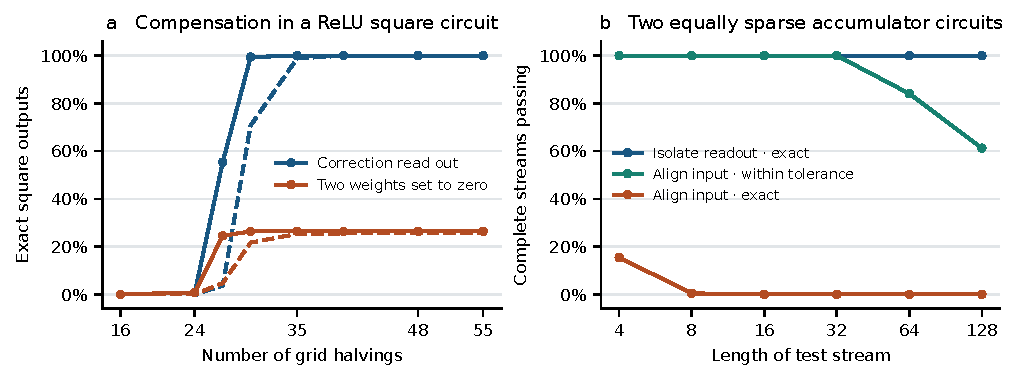
\includegraphics[width=\linewidth]{precision.pdf}
\caption{Two ways that a real-arithmetic identity can lose exact numerical agreement. Panel a varies the number of square refinements. Dashed lines use 4,096 central inputs, solid lines 8,192 outer inputs. The two networks differ only in whether the readout uses the accumulated rounding residual. Panel b compares two running-sum updates of width eight from Section~\ref{sec:front}. At each length, 64 initial networks are evaluated on the same 64 outer streams. Exact requires equality at every step. The tolerance curve requires $|\hat y-y|\le10^{-10}(1+|y|)$ at every step, where $y$ is the reference prefix sum and $\hat y$ the predicted sum.}\label{fig:prec}
\end{figure}

In a different experiment Astra received the square rule and could choose both the connections and coefficients of an affine/ReLU graph. It received no rounding-boundary failures before answering. One of three first replies computed the correctly rounded square for \emph{every} binary64 input in the two outer intervals using 2,543 input-dependent operations. Its graph extracts the significant digits, forms their integer product in three fixed-size pieces, and retains enough discarded information to round once at the end. Appendix~\ref{app:literal-square-certificate} proves the claim and gives an interior counterexample. We then added a rounding path for \emph{subnormal} results, the small-magnitude values below the smallest positive normal number in magnitude, with uniform spacing $2^{-1074}$. The engineered WSP graph uses 3,352 operations and is correct on all binary64 inputs in $[-10,10]$ (Appendix~\ref{app:fullsquare}). Both size counts are achieved upper bounds. The minimum for a deep graph remains open.

\paragraph{Sine, self-power and hyperbolic tangent.}
Our engineered WSP circuits for sine and positive self-power use affine operations and ReLUs. Their respective 500 and 1,352 stored coefficient words are individually addressable binary64 values. At inference both circuits matched the correctly rounded mathematical target on 32,768 fresh outer inputs, giving zero RMSE on those draws. We also used CORE-MATH, a project publishing difficult inputs for correctly rounded mathematical functions. The sine circuit missed 12 of 30,326 hard cases in its design interval $[-16,16]$ and one of the 1,884 in the requested shell. The self-power circuit missed 450 of 896 inputs chosen near output rounding boundaries just below one. Each miss was one adjacent representable value. The WSP hyperbolic tangent matched all 60,574 signed CORE-MATH cases in $[-10,10]$. Appendices~\ref{app:smooth-circuits} and \ref{app:relu-tanh} give run sizes and raw errors. On the deployed self-power and hyperbolic-tangent graphs, none of three BP fits per graph came within one ULP on an outer example after 100 Adam updates. The best of the three hyperbolic-tangent fits still achieved outer RMSE about 0.095. Tested hard cases establish measured accuracy for these circuits. Global correctness of their last output digit remains open.

\paragraph{Sorting without perturbing an input.}
For each ordering of four distinct real inputs, sorting applies a different permutation of the four coordinates. On the region corresponding to that ordering the derivative matrix (Jacobian) is the associated permutation matrix. A feedforward affine/ReLU graph with $g$ scalar ReLUs has at most $2^g$ patterns of active units and therefore at most $2^g$ distinct Jacobians on open regions. As $4!=24$, at least five gates are necessary. Five suffice over the reals: a \emph{comparator} sorts a pair $(a,b)$ by forming $t=R(a-b)$ and returning $(a-t,b+t)$. Applying it to five prescribed pairs sorts four inputs \cite{batcher1968sorting}. Subtracting a rounded difference can perturb one operand in binary64. In the fixed-schedule outer test this WSP sorter matched 1,105 of 2,048 lists with RMSE $5.12\times10^{-16}$.

A different comparator uses 13 ReLUs to select and transmit an original operand. It has 50 stored coefficients shared across comparisons. Sorting four inputs uses 65 ReLU executions, with 250 coefficient uses. Appendix~\ref{app:sort} proves that the comparator returns both original numerical values in order for every binary64 pair in $[-10,10]^2$, with signed zeros treated as equal. The resulting four-item WSP sorter had zero RMSE on the outer test. Five matched BP fits had median RMSE 4.35 and zero exact outer lists at the median. This gives a binary64 upper bound on gate count. The five-gate lower bound above concerns real arithmetic.

\section{How the sine and self-power circuits compute their outputs}
\label{app:smooth-circuits}

\paragraph{Circuits and reference values.}
We designed one circuit for the sine of a scalar input $x$ in radians on $[-16,16]$ and one for the self-power function $x\mapsto x^x$ on $[0,128]$, setting $0^0=1$ by continuity. Each design uses the formula and its domain. In this engineered weight-space programming (WSP) condition, we set the weights of each graph before evaluating any test input. The circuit is a directed acyclic graph, meaning a list of operations in which each result depends only on earlier operations. Its operations are scalar affine maps (weighted sums plus offsets) and rectified linear units, $\relu(v)=\max(0,v)$ for scalar $v$. We checked that at least one argument of every multiplication depends only on fixed coefficients. The graph uses separate binary64 operations, each rounded to nearest with ties to even. This fixes the order of addition and multiplication and permits subnormal results, the values spaced $2^{-1074}$ apart below the smallest positive normal number $2^{-1022}$.

Our mathematical reference is the exact function rounded once to binary64. We computed it with GNU MPFR version 4.2.2, a multiple-precision library with correctly rounded elementary functions~\cite{mpfr}, at 53 significant bits and cross-checked challenge values by rounding higher-precision evaluations. NumPy, the numerical library used in the earlier tests, differs from MPFR on 321 of the 8,192 ordinary outer sine inputs and 3 of the 4,096 ordinary outer self-power inputs. Here an exact match means agreement with MPFR. For the unit-in-the-last-place (ULP) distance we count representable steps between prediction and reference, identifying signed zeros.

\paragraph{Choosing a bit using rectified linear units.}
Let $r$ be a nonnegative binary64 remainder, $k$ an integer exponent used by the circuit and $a=2^k$ a normal threshold. Its nearest smaller binary64 value is $a-2^{k-53}$. Define the threshold gate
\[
 B_k(r)=\relu\!\left(1-\relu\!\left(2^{53-k}(a-r)\right)\right).
\]
At $r\ge a$ the inner rectifier returns zero. At $r<a$ the gain $2^{53-k}$ scales the difference to at least one. Thus the output is precisely the bit for the decision $r\ge a$. To copy a signed value $v$ only when a bit $b$ equals one, choose a bound $M\ge |v|$ and evaluate $\relu(v-M(1-b))-\relu(-v-M(1-b))$. The result is $v$ when enabled and zero otherwise. The circuit uses these operations to select terms of known sums. Its two-word variant represents an intermediate by the sum of a leading binary64 value and a smaller correction. Compensated arithmetic retains part of the rounding error of each sum or constant product in that correction~\cite{dekker1971}.

\paragraph{Sine.}
Starting with angle zero, we store its sine and cosine, zero and one. We inspect the powers $2^k$ in $|x|$ from $k=4$ downward. Whenever $B_k$ selects a power, we subtract it from the remainder and apply the sine and cosine angle-addition formulas for a rotation of $2^k$ radians. Its sine and cosine are coefficients computed before inference by Taylor series for angles up to one radian and angle doubling for larger angles. The 83-stage graph ends at $k=-78$ and restores the sign of $x$. For $|x|\le 2^{-26}$ it returns $x$ directly, because the bound $|x-\sin x|\le |x|^3/6$ is below half the distance to the next binary64 value toward zero.

\paragraph{Self-power.}
For $x\ge 2^{-64}$, choose an integer exponent $e$ and fractional remainder $u$ with $x=2^e(1+u)$ and $0\le u\le 1$. Write $\log$ for the natural logarithm. At fractional digit $j$, starting at $j=1$, let $d=2^{-j}$. When the leading word of $u$ reaches $d$, multiply $u-d$ by the stored coefficient $1/(1+d)$ and add the stored $\log(1+d)$ to a running logarithm initialized at $e\log 2$. The identity $(1+u)/(1+d)=1+(u-d)/(1+d)$ explains the update. After the last digit, add the remaining $u$ as a first-order approximation to $\log(1+u)$. Next form $y=1+x\log x$ by adding scaled copies of that logarithm for the selected input bits. Finally, start at $\exp(-1)$, where $\exp$ is the natural exponential, and multiply by the stored $\exp(2^k)$ for each selected bit of $y$. The exact-arithmetic identity is $\exp(-1)\exp(y)=x^x$. For $x<2^{-64}$ the circuit returns one. These digitwise logarithm and exponential methods have precedents in elementary-function algorithms \href{https://doi.org/10.1109/12.295857}{(Bajard, Kla and Muller, 1994)}.

\paragraph{Comparing sizes.}
We count separately a stored coefficient, an occurrence of a coefficient in an expanded affine operation, and an executed rectifier. The engineered WSP graphs for 83-stage sine and 84-fractional-bit self-power store 500 and 1,352 coefficient words. Each word overwrites a scalar Xavier draw, uniform on $[-\sqrt{3},\sqrt{3}]$. The topology and fixed signs already encode the algorithm. Expanding repeated coefficient uses gives 25,395 and 35,908 affine occurrences and 1,506 and 2,618 rectifiers. The affine count charges two coefficients for a sum of two variables or a variable plus an offset and one for scaling. The stored graphs also have four and seven fixed structural constants respectively. Figure~\ref{fig:smooth-relu} identifies the first tested sizes to pass the ordinary outer samples. Smaller unswept graphs could have the same accuracy.

\begin{figure}[htbp]
\centering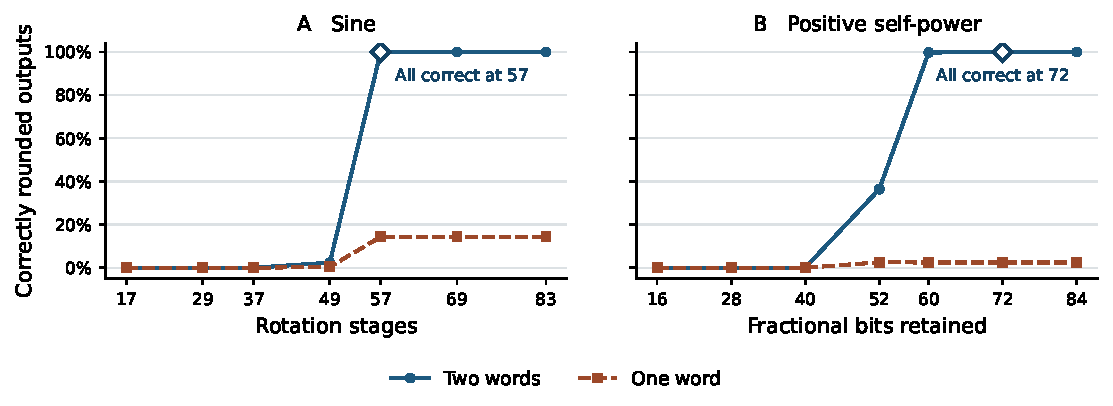
\includegraphics[width=.97\linewidth]{smooth_precision.pdf}
\caption{Fraction of inputs for which the network returns the correctly rounded mathematical value. The sine panel pools 4,096 inputs from each of $[-10,-3]$ and $[3,10]$. The self-power panel uses 4,096 inputs from $[3,10]$. Each curve evaluates the same inputs at seven sizes. The solid curve stores a leading word plus a rounding correction, and the dashed curve uses one word per intermediate. An open diamond marks the first sampled size with no misses in each panel. At 60 fractional bits, the two-word self-power circuit still misses 10 of 4,096 inputs.}
\label{fig:smooth-relu}
\end{figure}

\paragraph{Where agreement fails.}
At 57 sine stages (344 stored words) and 72 fractional bits for self-power (1,208 words), the two-word circuits first matched their respective full ordinary outer samples. The two largest WSP circuits also matched all 4,096 central and 32,768 independently drawn outer inputs per task, plus 8,192 inputs per task with exponents sampled uniformly into the subnormal range. Both had zero raw root mean squared error (RMSE) on the ordinary central and outer sets. Sine matched 102 values near nonzero multiples of $\pi$ (half a turn in radians) and 4,096 farther inputs in $[10,16]$. Self-power matched 213 values at or adjacent to powers of two and 4,096 farther inputs in $[10,128]$.

CORE-MATH is a public project that distributes inputs whose function values are hard to round correctly. On its sine inputs the largest graph misses 12 of 30,326 distinct values in $[-16,16]$, including one of 1,884 in the requested outer intervals. Each miss is one representable step. Across all 30,326 hard inputs the RMSE is $7.31\times10^{-19}$, and on the 1,884 hard outer inputs it is $2.50\times10^{-21}$. We write inputs as hexadecimal significands times powers of two, with \texttt{p} introducing the base-two exponent. At $x=\texttt{0x1.9239c4bbb44a4p+1}$ the absolute error is $1.08\times10^{-19}$ and the absolute error divided by $|\sin x|$ is $1.36\times10^{-16}$. The archive records the source revision and file hash for the \href{https://core-math.gitlabpages.inria.fr/worst.html}{public input corpus}.

For self-power, values just below one are spaced $2^{-53}$ apart. For integers $j=0,\ldots,127$, we located the small positive input satisfying $x\log x=\log(1-(j+1/2)2^{-53})$. Its exact output is a midpoint between two binary64 values. We tested the closest binary64 input and its three neighbors on either side. Of 896 outputs, 446 matched and the remaining 450 were one step away. At $x=\texttt{0x1.8e2e5fb51604cp-60}$ the network returns one. The reference is the next value below one, an absolute difference of $2^{-53}$. The RMSE across the 896 near-midpoint inputs is $7.87\times10^{-17}$.

\paragraph{Gradient and product-gate controls.}
On the same 83-stage sine graph, we trained all 500 slots with adaptive moment estimation (Adam), using gradients propagated backward from the loss. We gave the optimizer 1,024 central labels, three independent Xavier starts, 100 updates at learning rate $0.01$ and 32 observations per update. Respectively two, two and zero slots changed, and each run matched zero outer outputs exactly. Outer RMSE in seed order was 16.51, 8.14 and 15.96, compared with zero for the same WSP graph. A separate comparison allowed products of two input-dependent values. We fitted a degree-65 odd polynomial by full-batch Gauss--Newton updates (least-squares updates to the locally linear predictions) in a Chebyshev basis (polynomials orthogonal on a rescaled central interval under the Chebyshev weight). We evaluated both this fit and the formula-written Taylor coefficients with Horner's rule, which alternates multiplication by the argument with addition of a coefficient. Using two words for each of its 33 odd-power coefficients, the formula-written network matched all 8,192 ordinary outer sine values but missed 68 of the 102 probes near roots. The central-label fit matched none of the 8,192 and had outer RMSE $1.13\times10^{35}$, compared with zero for the Taylor coefficients. The electronic tables in \path{revision/numeric_metrics/} retain raw RMSE and exact counts for each size, split and fitted control.

\section{Computing the hyperbolic tangent with affine maps and rectifiers}
\label{app:relu-tanh}
For a real input $x$, the hyperbolic tangent is $\tanh x=(e^{2x}-1)/(e^{2x}+1)$, with $e$ the base of the natural logarithm. The native one-neuron control in the earlier controls (Appendix~\ref{app:additional}) reproduces the NumPy library's implementation. Here both NumPy and a weight-space programming (WSP) circuit are compared with the mathematical function correctly rounded by MPFR. The WSP circuit receives the formula and the domain $[-10,10]$.

\paragraph{Building a ratio from the input bits.}
For an integer exponent $k$, set the angle $\delta=2^k$. Before inference we compute the coefficient $t_k=\tanh\delta$ at 256-bit precision. We use $t_k=\operatorname{expm1}(2\delta)/(2+\operatorname{expm1}(2\delta))$, where $\operatorname{expm1}(z)=e^z-1$ is evaluated accurately for small $z$. Let $K$ be the number of fractional input-bit positions inspected. Read the bits of $|x|$ for $k=3,2,\ldots,-K$. Keep a numerator $N$ and denominator $D$ initialized to zero and one. When the bit for $\delta$ is one, update both using their previous values,
\[
             (N,D)\longleftarrow (N+t_kD,\ D+t_kN).
\]
The addition formula makes $N/D$ the hyperbolic tangent of the sum of selected angles in exact arithmetic. To copy a signed intermediate $z$ with $|z|\le128$ when a bit $b$ is one, the circuit uses $\relu(z-128(1-b))-\relu(-z-128(1-b))$. Each exact update grows the maximum magnitude of the coordinates by at most $1+t_k$. The factors for the four nonnegative exponents give a product at most 16. The factors for negative exponents give a product at most $\exp(\sum_{k<0}2^k)=e$. These bounds motivate the choice of 128.

\paragraph{Quotient digits and rounding.}
Start with a remainder $R=N$. At fractional position $j=1,2,\ldots$, the next quotient digit is one if $R\ge 2^{-j}D$. Subtract $2^{-j}D$ from $R$ whenever this comparison succeeds. The final circuit keeps the first 53 significant quotient bits beginning with the first one, and inspects the following bit, called the guard bit. If it is one, the circuit adds one unit at the last retained position. To see why the mathematical target has no tie at nonzero binary64 inputs, suppose $\tanh x$ were the midpoint between two consecutive representable values, which is a rational number. Then $e^{2x}=(1+\tanh x)/(1-\tanh x)$ would be rational. The Hermite--Lindemann theorem says the exponential of a nonzero algebraic number is transcendental, meaning it cannot be a root of a nonzero polynomial with integer coefficients. The nonzero rational number $2x$ meets the theorem's hypothesis. Finite-precision comparisons can still produce an incorrect bit.

For $|x|\le 2^{-27}$, a final gate copies $x$ because $0\le |x|-\tanh|x|\le |x|^3/3$ lies below half the spacing toward zero. For larger magnitudes the circuit restores the sign of $x$ after extracting the quotient. The 84-fractional-bit construction uses 82 quotient positions. The input and quotient digit counts are distinct. Each coordinate uses three binary64 words representing a leading part and two corrections. The circuit combines rounded sums, constant products and their rounding residuals, recording successive corrections across the words. It stores 525 coefficient words and uses 2,146 rectifiers. Expanding repeated uses and fixed unit edges gives 75,973 affine coefficient occurrences. A traversal of the graph checks that every product has an input-independent factor.

\paragraph{Evaluation.}
The ordinary central set contains 4,096 inputs in $[-3,3]$. The ordinary outer set contains 4,096 per side in $[-10,-3]$ and $[3,10]$. A fresh draw contains 32,768 additional outer inputs. To construct targeted tests, take adjacent representable output values, compute their midpoint, and invert it at 240-bit precision using the inverse hyperbolic tangent, $\operatorname{atanh}$. Test the nearest input and its two neighbors with both signs. These give 4,608 central and 4,608 outer examples. Finally, use the independently selected \href{https://core-math.gitlabpages.inria.fr/worst.html}{CORE-MATH hard inputs}. The 53-bit MPFR results agree with the cross-check at 224 bits rounded to binary64.

\begin{table}[htbp]
\centering\small
\caption{Exact matches to correctly rounded hyperbolic tangent. Every miss is one representable step. The hard columns use signed CORE-MATH inputs. The last two rows use 84 fractional input positions and direct guard-bit rounding.}
\label{tab:relu-tanh}
\begin{tabular}{@{}lrrrrrr@{}}\toprule
Method & Central & Outer & Fresh outer & Midpoint & Hard central & Hard outer\\
Inputs & 4,096 & 8,192 & 32,768 & 9,216 & 57,060 & 3,514\\\midrule
Native NumPy & 3,276 & 6,268 & 25,285 & 5,458 & 42,710 & 2,660\\
Two-word WSP & 4,096 & 8,192 & 32,768 & 9,216 & 57,024 & 3,512\\
Three-word WSP & 4,096 & 8,192 & 32,768 & 9,216 & 57,060 & 3,514\\\bottomrule
\end{tabular}
\end{table}

For the three methods in Table~\ref{tab:relu-tanh}, raw root mean squared error (RMSE) on the ordinary outer inputs is $5.38\times10^{-17}$, zero and zero, respectively. On the hard outer inputs it is $5.47\times10^{-17}$, $2.65\times10^{-18}$ and zero. The electronic results give exact counts and raw RMSE for every method, size and input set. In the earlier two-word variant, summing 120 quotient digits gives 55,896 of 57,060 hard central and 3,512 of 3,514 hard outer matches. In the three-word size sweep, $K=79$ misses two hard central inputs and two inputs near selected boundaries. At $K=80$ all tested outputs match using 503 stored words and 2,068 rectifiers. This establishes an observed size threshold within the tested family. A proof covering every in-domain binary64 input remains open.

\section{How closely can gradients fit the same self-power and tanh circuits?}
\label{app:smooth-optimizer}
We exposed all 1,352 stored coefficients of the positive self-power circuit and all 525 of the three-word hyperbolic tangent circuit to backpropagation (BP). The wiring, operation order and fixed numerical constants were those of the deployed WSP circuits. The three trials initialized every exposed coefficient by a scalar Xavier draw with seeds 11, 22 and 33. The objective was mean squared error (MSE), the mean squared difference between prediction and correctly rounded output on 1,024 central inputs. A training update sampled 32 pairs with replacement. Reverse-mode differentiation propagated derivatives of the separate operations back to the weights, taking derivative zero at the rectifier's kink. Adam made 100 updates with step size $0.01$. Its decay rates for first and second gradient moments were $\beta_1=0.9$ and $\beta_2=0.999$. The stabilizer in the update denominator was $\epsilon=10^{-8}$. The targets came from MPFR, with higher-precision cross-checks. We scored the final iterate.

\begin{table}[htbp]
\centering\small\setlength{\tabcolsep}{4pt}
\caption{Training all exposed slots with BP and Adam. Training MSE is evaluated over all 1,024 central examples before and after fitting. A moved slot differs from its initial value. The maximum gradient is the largest absolute partial derivative of the batch objective over all slots and updates. Outer RMSE is in the output's original units against MPFR (4,096 self-power or 8,192 tanh inputs).}
\label{tab:smooth-gradients}
\begin{tabular}{@{}lrrrrrr@{}}\toprule
Target & Seed & Initial MSE & Final MSE & Moved slots & Max.\ gradient & Outer RMSE\\\midrule
Self-power & 11 & 68.2141 & 59.0062 & 2 & 59.6 & $1.46\times10^9$\\
 & 22 & 59.0175 & 59.0123 & 2 & 0.0822 & $1.46\times10^9$\\
 & 33 & 68.3098 & 67.7551 & 74 & 11.7 & $1.46\times10^9$\\
Tanh & 11 & 75.9257 & 1.72681 & 439 & $2.44\times10^6$ & 1.50\\
 & 22 & 11,772.6 & 6,168.13 & 373 & $2.52\times10^6$ & 103.83\\
 & 33 & 26.2714 & 0.062064 & 292 & $1.75\times10^4$ & 0.0953\\\bottomrule
\end{tabular}
\end{table}
On these same examples, both WSP circuits had zero training MSE and zero outer RMSE, matching every reference output. Each of the six gradient fits in Table~\ref{tab:smooth-gradients} returned zero exact outer outputs and zero within one ULP. Every update had finite loss, gradients and optimizer state. In each run the slots whose gradients were ever nonzero were exactly those whose final values changed. With seed 33 the tanh network reduced its outer mean absolute error to 0.0711 while moving 292 slots. This comparison measures achieved accuracy at three starts and the stated training budget.

\begin{table}[htbp]
\centering\small\setlength{\tabcolsep}{5pt}
\caption{Outer predictions on the same graph and the same inputs for each target. WSP uses the stored coefficients of the deployed circuit. BP and Adam fit these slots from Xavier draws using 100 updates. The reported BP RMSE is the median of the three seed-specific raw RMSE values. Every seed has the exact-match count shown.}
\label{tab:matched-smooth-rmse}
\begin{tabular}{@{}lrrrrr@{}}\toprule
Target & Outer inputs & WSP exact & BP exact & WSP RMSE & BP RMSE\\\midrule
Sine & 8,192 & 8,192 & 0 & 0 & 15.96\\
Self-power & 4,096 & 4,096 & 0 & 0 & $1.46\times10^{9}$\\
Hyperbolic tangent & 8,192 & 8,192 & 0 & 0 & 1.50\\\bottomrule
\end{tabular}
\end{table}

\section{A recurrent network that executes branching instructions}\label{app:machine}
A register machine stores a nonnegative integer in each register and executes one instruction at a time. Its program counter identifies the active instruction. Let $r$ index a register, let $z_r$ be its current value, and let $k,k_0,k_+$ index destination instructions. The increment instruction $\mathrm{INC}(r,k)$ adds one to $z_r$ and jumps to $k$. The conditional decrement $\mathrm{DECJZ}(r,k_0,k_+)$ jumps to $k_0$ if $z_r=0$. Otherwise it subtracts one and jumps to $k_+$. The halt instruction holds the complete state fixed. With unbounded integer counters and time, these instructions include a universal two-counter machine, which can simulate any Turing-computable procedure under an appropriate encoding~\cite{dudenhefner2022machines}. Binary64 cannot distinguish the adjacent register values $2^{53}$ and $2^{53}+1$. We examine both an exact-arithmetic instruction identity and finite binary64 executions. Related work characterizes when learned rectifier cells count exactly~\cite{elnaggar2023counting}.

\paragraph{One update per instruction.}
Let $R$ be the number of registers, $P$ the number of instructions, $G$ the number of conditional decrements, and $d=R+P$ the number of stored coordinates. Append to the register values a one-hot vector of $P$ instruction indicators, with entry $p_j$ equal to one for the active instruction $j$ and zero for the others. Write $z\in\mathbb{R}^d$ for the resulting state and $z'$ for the next state. Let $D$ be a $d\times d$ matrix that directly updates the state, $W$ a $G\times d$ matrix testing conditional instructions, and $E$ a $d\times G$ matrix routing the branch corrections. With a componentwise rectifier, one update is
\[
       z'=\relu\bigl(Dz+E\relu(Wz)\bigr).
\]
The register block of $D$ copies each register. Its column for an increment adds one to the named register and places the active bit at the destination. Its halt column retains the current instruction bit. For a conditional decrement of register $r$ at instruction $j$, the corresponding hidden unit computes $\relu(p_j-z_r)$. This equals one precisely when this instruction is active and the register value is zero. The corresponding column of $D$ attempts a decrement and selects the positive destination. A unit hidden bit switches the destination through $E$. It can also cancel the attempted decrement. Alternatively the outer rectifier clips the attempted $-1$ to zero. In both cases every legal integer state advances exactly one instruction under exact arithmetic. Induction gives the specified states at every finite time.

\begin{table}[htbp]
\centering\small\setlength{\tabcolsep}{4pt}
\caption{Five instruction lists compiled independently of the Astra trials. A dense slot is one matrix entry, including zero entries. The last column sums the number of executed instructions, or ticks, over all outer inputs. Every intermediate state and final scalar matched the integer interpreter, giving raw RMSE zero on each of these five outer sets.}
\label{tab:register-circuits}
\begin{tabular}{@{}lrrrrrr@{}}\toprule
Target & Registers & Instructions & Branch gates & Dense slots & Outer inputs & Total ticks\\\midrule
Addition & 2 & 3 & 1 & 35 & 49 & 735\\
Truncated subtraction & 2 & 3 & 2 & 45 & 49 & 644\\
Multiplication & 4 & 7 & 3 & 187 & 49 & 13,083\\
Triangular number & 3 & 8 & 3 & 187 & 7 & 1,008\\
Fibonacci number & 4 & 9 & 4 & 273 & 7 & 2,860\\\bottomrule
\end{tabular}
\end{table}

The integer interpreter in Table~\ref{tab:register-circuits} determined how many updates to score. The recurrent cell evolved autonomously from each initial state. Inputs ranged over all tuples from $\{0,1,2,3\}$ centrally and $\{4,\ldots,10\}$ on the outer set. For nonnegative integers $a,b$, truncated subtraction returns $\max(a-b,0)$. In a separate test, six fresh Astra calls each received a relabeled two-register, four-instruction list and Xavier-initialized matrices. Across the calls we changed two branch wirings and permuted the state coordinates. All six replies gave the clipped-decrement construction up to gate and coordinate permutations. Each passed every one of 196 outer one-step states and 64 traces of 128 steps, with zero state RMSE. The six trials share two instruction structures.

\paragraph{Learning the transitions.}
For addition, truncated subtraction and multiplication, we trained every continuous weight on central one-step input--output labels from three Xavier starts. On each task, zero of the three BP fits produced any entirely exact outer trace. For the final scalar on each of the 49 outer inputs, median raw RMSE across starts was 10.60, 2.00 and 45.99 respectively. The corresponding WSP compiler and a solver that inferred the discrete instruction table from the central labels both had zero RMSE. One fitted multiplication cell produced the right rounded next state on all 16,807 outer one-step cases, while none of its 49 autonomous final scalar outputs matched. We rounded the single-step prediction only for this diagnostic. Autonomous execution passed the unrounded state to the next update. The electronic tables distinguish one-step state error, state error pooled across ticks and coordinates, and final scalar error.

\section{Choosing both the operations and the weights}\label{app:synthesis}
We asked whether Astra could implement square, sine or positive self-power when it could choose the circuit topology, meaning the operations and their connections. A domain-specific language (DSL) restricted the allowed operations. Each reply was an instruction list written in JavaScript Object Notation (JSON), a text format for structured data. A wire carries the value computed at one graph node. An input-dependent wire can vary with the input, while an input-independent wire carries a fixed constant. The affine/rectifier operator set permits addition, subtraction, multiplication by an input-independent constant, division by a constant and rectification. A second operator set also permits products of two input-dependent wires. In both sets, constants can use sine, logarithms and other elementary functions when the graph is built. For each unseen input, inference executes only the resulting fixed circuit. Every operation that depends on the input counts once toward the 4,096-operation cap after expansion of loops with fixed bounds. Precomputed constants, the size of the instruction text and the number of wires are separate costs.

Each prompt supplied the target formula, input interval, arithmetic rules and operation cap. Eighteen independent requests covered three targets, two operator sets and three replicate labels (9213, 2451 and 8282). The labels distinguish calls with the same instruction, without changing their inputs. The model returned weights and topology without a given Xavier array, tools, examples or evaluation feedback. In the affine/rectifier self-power condition two requests timed out after 300 seconds. We repeated those two before scoring, with a 900-second limit. One reply had invalid JSON syntax and the other exceeded the operation cap. Neither produced an evaluable circuit. All 16 responses returned within the original budget compiled. Table~\ref{tab:circuit-synthesis} keeps all 18 conditions.

\begin{table}[htbp]
\centering\small\setlength{\tabcolsep}{4pt}
\caption{WSP with free topology. For each trial the accuracy columns count exact outputs out of 16,384 outer inputs against correctly rounded MPFR values. Sine and square use both signs with magnitudes from 3 to 10, and self-power uses positive inputs. The last column gives the number of input-dependent operations in trial order. An invalid reply has no numerical prediction or RMSE.}
\label{tab:circuit-synthesis}
\begin{tabular}{@{}llrrrl@{}}\toprule
& & \multicolumn{3}{c}{Exact outer predictions} & Operation counts\\
Target & Operators & Trial 1 & Trial 2 & Trial 3 & Trials 1, 2, 3\\\midrule
Square & Affine/ReLU & 16,384 & 16,384 & 16,384 & 2543, 4081, 2833\\
Square & With product & 16,384 & 16,384 & 16,384 & 1, 1, 1\\
Sine & Affine/ReLU & 8,191 & 9,272 & 5,662 & 4067, 3959, 3790\\
Sine & With product & 16,384 & 16,384 & 16,384 & 587, 526, 772\\
Positive self-power & Affine/ReLU & 0 & invalid & invalid & 4026, invalid, invalid\\
Positive self-power & With product & 16,384 & 16,384 & 16,380 & 2622, 3008, 2881\\
\bottomrule
\end{tabular}
\end{table}

On these same outer sets the three affine/rectifier sine circuits have raw RMSE $1.47\times10^{-16}$, $1.03\times10^{-16}$ and $1.07\times10^{-16}$. For affine/rectifier self-power, the sole valid circuit has RMSE 0.0166. With product gates, the third self-power circuit has RMSE $1.18\times10^{-13}$. All other evaluable rows and trials in Table~\ref{tab:circuit-synthesis} have RMSE zero. Each product-gate square reply uses a single binary64 multiplication, which computes the reference by definition.

Every affine/rectifier square proposal matched all 304 inputs specially chosen near rounding midpoints on the outer intervals and all 32,768 fresh ordinary outer inputs. Across 16,369 inputs sampled over a wider range of exponents, the three exact counts were 16,357, 16,294 and 16,364. Appendix~\ref{app:literal-square-certificate} proves the first circuit's result on both complete outer intervals. On 1,884 CORE-MATH sine inputs in those intervals the three affine/rectifier replies matched 1,026, 1,079 and 697, compared with 1,881, 1,884 and 1,883 with product gates. The product-gate self-power circuits missed one, one and two of the 896 near-midpoint probes below one defined in Appendix~\ref{app:smooth-circuits}. On the 8,192-input wide-exponent panel, the second and third product-gate self-power replies each produced nonfinite outputs, so neither has finite raw RMSE there. The electronic results retain each trial, split, exact count and RMSE status. In this experiment Astra chose each topology. The same-graph BP comparisons in Appendix~\ref{app:smooth-optimizer} concern the three separately engineered smooth circuits.

\section{What changes after one round of central feedback?}
\label{app:repair}
For each of the three scalar targets and two operator sets in Appendix~\ref{app:synthesis}, we selected the first trial in advance using its replicate label, 9213. This gives six pairs of circuits. Each follow-up request included the original specification, the verbatim first reply, and a diagnostic computed on all 4,096 central inputs. For an executable circuit the diagnostic listed operation count, number of finite outputs, exact matches and matches at distance at most one ULP (including exact matches). It supplied the input, prediction and reference for only the three largest ULP errors. Nonfinite predictions received priority and the earlier input broke ties. If every case matched, the three supplied examples all showed equality. For a circuit that failed to compile, the prescribed diagnostic was the parser error and the first three central labels. Astra could return its previous answer. Each revision used one separate medium-effort Astra request with a 300-second timeout and the same 4,096-operation cap. The six requests contained only this central feedback.

\begin{table}[htbp]
\centering\small\setlength{\tabcolsep}{3.5pt}
\caption{Effect of one WSP revision given central feedback. An arrow separates the first result from the revised one, and a single number denotes equality before and after. The operations column counts input-dependent operations. The other columns count exact matches to MPFR. Both circuits were evaluated on identical inputs. The existing outer sample was used for the first-response study. The fresh sample was drawn with an independent seed.}
\label{tab:repair}
\begin{tabular}{@{}llrrrr@{}}\toprule
Target & Operators & Operations & Central (4,096) & Outer (16,384) & Fresh (32,768)\\\midrule
Square & Affine & 2,543 & 4,096 & 16,384 & 32,768 \\
Square & Product & 1 & 4,096 & 16,384 & 32,768 \\
Sine & Affine & 4,067 $\to$ 3,878 & 2,055 $\to$ 3,185 & 8,191 $\to$ 11,650 & 16,126 $\to$ 23,157 \\
Sine & Product & 587 & 4,096 & 16,384 & 32,768 \\
Self-power & Affine & 4,026 $\to$ 4,049 & 1 $\to$ 797 & 0 $\to$ 1,088 & 2 $\to$ 2,265 \\
Self-power & Product & 2,622 $\to$ 3,358 & 4,096 & 16,384 & 32,768 \\
\bottomrule
\end{tabular}
\end{table}

All six revisions compiled. The recorded interaction for each has one model reply and no tool action. Three replies were byte-for-byte identical to the originals. Requests took 5.8--139.6 seconds. For affine/rectifier sine, 9,608 fresh outer inputs became exact while 2,577 formerly exact predictions changed to a neighboring or more distant float. Across those same 32,768 inputs, raw RMSE fell from $1.47\times10^{-16}$ to $5.07\times10^{-17}$. For affine/rectifier self-power it fell from 0.0163 to $6.32\times10^{-6}$, with maximum ULP distance falling from 324,964 to 187. The other four pairs matched every fresh outer output and had RMSE zero before and after repair. The electronic table records all four evaluated splits, including a fresh central set. A single feedback round measures these six specific revisions, conditional on the first reply and the three cases shown.

\section{A first-response ReLU square correct on the entire outer shell}
\label{app:literal-square-certificate}
We prove the following all-input statement for a first response in the free-topology WSP experiment. We analyzed the frozen reply \texttt{3354251e2} (replicate 9213, 2,543 expanded input-dependent operations). The graph multiplies a wire only by a fixed coefficient. A loop implements integer multiplication using affine operations and ReLUs. Let $\mathrm{RN}$ denote binary64 rounding to nearest, ties to even. Under the separate-operation contract of the circuit language in Appendix~\ref{app:synthesis}, this reply returns $\mathrm{RN}(x^2)$ for \emph{every} binary64 $x$ with $3\le |x|\le10$.

\paragraph{Normalization.}
Initialize a nonnegative remainder $r$ to $r_0=|x|/16\in[3/16,5/8]$, exactly representable in this range. In decreasing order of the integer index $j$, a flag $f_j$ records whether to rescale $r$. The flags at thresholds $a=2^{-j}$, for $j=512,256,128,64,32,16,8,4,2,1$, test $r<a$ by
\[
 f_j=\relu\!\left(1-2^{j+53}\relu(r-(a-2^{-j-53}))\right).
\]
The stored threshold in the inner subtraction is the predecessor of $a$. If $r<a$ then $r$ is at most that predecessor, giving $f_j=1$. At $r=a$ the subtraction is exactly $2^{-j-53}$. For every representable $r\ge a$, monotonic rounding gives a difference at least that large, hence $f_j=0$. Even the largest gain has finite product on this shell. With intermediate $h=\relu(r-f_j)$, the update $r\gets h+(r-h)2^j$ therefore preserves $r$ for a zero flag and scales $r$ by $2^j$ for a unit flag, since $0\le r\le1$. The flags through $j=4$ vanish. Those at $j=2,1$ normalize $r_0$ into $r\in[1/2,1)$ by factors four, two, or one. Thus $m=2^{53}r$ is an exactly represented integer in $[2^{52},2^{53})$.

\paragraph{Exact integer square.}
Use the integer base $B=2^{27}$. A limb is a digit in this base. The first loop reads the 26 highest-order binary digits of $m$, where higher order means greater place value. It obtains the integer quotient $a=\lfloor m/B\rfloor$ and remainder $b=m-aB$. For an integer remainder $u$ and power of two $p$, the bit test $\relu(1-\relu(p-u))$ returns one if $u\ge p$ and zero otherwise. The next loop reads all 53 bits of $m$ from most to least significant. Let $v$ denote the integer represented by the bits already read. Let $P$ denote their product with $m$, and $H$, $M$ and $L$ its high, middle and low limbs. After each prefix, the stored values satisfy
\[
 P=vm=H B^2+M B+L,\qquad 0\le M,L<B .
\]
Initially all limbs are zero. For bit $t$ the updated product should be $2P+tm$. The two lower limbs add $tb$ and $ta$ respectively to the doubled old digits, with carry from the lower limb. The actual selectors $\relu(b-(1-t)B)$ and $\relu(a-(1-t)B)$ produce those summands exactly. Let $z$ denote either provisional digit sum before carrying. Both are integers in $[0,3B)$. The carry into the next digit is the quotient $\lfloor z/B\rfloor$. The circuit computes it by adding the two comparison bits at $B$ and $2B$, subtracts the resulting multiple of $B$, and adds the carry to the next digit. The high digit is updated as $2H+\mathrm{carry}$. Each prefix product satisfies $P\le m^2<2^{106}$, so $H<2^{52}$. The digit and bit operations stay within the binary64 exact integer range. After the last iteration $P=m^2$.

\paragraph{One final rounding.}
The normalized real square is $r^2=2^{-52}(H+M/B+L/B^2)$. Define the sticky bit $s$ to be one if any bit of the discarded low limb $L$ is nonzero, and zero otherwise. Let $v_{\mathrm{sq}}$ denote the rounded normalized square computed by the circuit,
\[
 v_{\mathrm{sq}}=2^{-52}\,\mathrm{RN}\!\left(H+\frac{M+s/2}{B}\right).
\]
Here $M+s/2$ and division by $B$ are exact. The integer $H$ lies in $[2^{50},2^{52})$. Throughout the possible range of $P/B^2$, binary64 rounding midpoints lie on the $1/B$ lattice (the intervals between successive powers of two in this range have spacings $1/4$ and $1/2$). If $L=0$, the unrounded argument is exact. If $L>0$, both $H+M/B+L/B^2$ and $H+(M+1/2)/B$ lie strictly inside the same interval between adjacent $1/B$ lattice sites. No rounding midpoint separates them. Thus replacing the low limb preserves the side of every midpoint, and $L=0$ preserves an exact tie and its even-neighbor decision. The final addition therefore produces the correctly rounded value of $P/B^2$. The circuit undoes each active normalization by an exact division by four or sixteen, then multiplies by 256 to undo the initial division of the input by sixteen. On the shell all these rescalings by powers of two remain normal, so rounding commutes with them and the result is $\mathrm{RN}(x^2)$.

The shell proof allows a concrete failure closer to zero. At $x=\texttt{0x1.0000000000001p-512}$ the same frozen circuit differs from the reference by one subnormal spacing. A separate audit against once-rounded exact rationals reproduced 104/104 normalization-boundary cases, 2,466/2,466 limb-boundary cases, 2,222/2,222 exact rounding ties, and 1,192/1,192 additional near-midpoint cases in the shell. All four finite panels had raw RMSE zero. The argument above supplies the all-shell guarantee.

\section{A separately engineered square circuit for every binary64 input in $[-10,10]$}
\label{app:fullsquare}
The first-response WSP square circuit in Appendix~\ref{app:literal-square-certificate} fails on some central inputs with normal outputs.
For the scalar input $x=(1+2^{-52})2^{-508}$ it returns $2^{-1016}$, two output ULPs below the correctly rounded square.
Its intermediate value represents $x^2/256$ before a final power-of-two rescaling.
We retain the first 2,492 scalar operations of that proposal and replace its output logic.
The resulting graph has 3,352 operations (949 ReLUs), compared with 2,543 operations (732 ReLUs) in the first reply.
Both graphs use the same operation-by-operation binary64 evaluator. These numbers give construction costs.

\paragraph{Claim.}
Let $x$ denote any binary64 input in $[-10,10]$. Use the binary64 format of the Institute of Electrical and Electronics Engineers (IEEE) standard, round each graph operation separately to nearest with ties to even, and retain subnormal results (gradual underflow). Write $\operatorname{RN}$ for this rounding. The engineered WSP graph returns the bit pattern of $\operatorname{RN}(x^2)$ for every such $x$, including both signed zeros.

\paragraph{Normalization.}
Initialize a running nonnegative remainder $r$ to $r_0=\operatorname{RN}(|x|/16)$. At each integer $k=512,256,\ldots,1$ in decreasing powers of two, define a flag $f_k$ to be one if the current $r<2^{-k}$ and zero otherwise. The shared prefix multiplies $r$ by $2^k$ exactly when the flag is set.
For $q=2^{-k}$ the preceding float is $q-\delta$ with $\delta=2^{-k-53}$. The implemented flag is
$\operatorname{ReLU}(1-\delta^{-1}\operatorname{ReLU}(r-(q-\delta)))$.
For $r\le q-\delta$ the inner ReLU is zero. For $r\ge q$, monotone rounding gives an inner difference at least $\delta$, so the flag is zero. All intermediates are finite since $r<1$ and $k\le512$.
The conditional update uses $h=\operatorname{ReLU}(r-f_k)$ and $r\gets h+(r-h)2^k$, with $h=r$ or $0$ exactly.
The strict threshold keeps $0\le r<1$ throughout.
Define the total rescaling exponent $S=\sum_k k f_k$. This integer also selects the output branch below. We obtain $r=r_0 2^S$.
For $r_0>0$ the descending flags perform the binary expansion of the integer shift taking $r_0$ into $[1/2,1)$, capped at 1023. For $r_0=0$, all flags are set.
If $S\le541$, the normalization reaches $[1/2,1)$ and the initial division by 16 is exact. Indeed, inexact division could only produce $r_0\le2^{-1022}$, which requires a shift of at least 1021.
Define the significand integer $m=2^{53}r$ and its exact square $P=m^2$. In this case $m$ lies in $[2^{52},2^{53})$ and
\[
 |x|=m2^{-49-S},\qquad x^2=P2^{-98-2S},\qquad P=m^2.
\]
Even if the shift saturates, $m$ is an integer below $2^{53}$ because $r_0$ is a multiple of $2^{-1074}$ and $1023+53\ge1074$.

\paragraph{Normal outputs, $S\le514$.}
Let $H,M,L$ be the high, middle and low digits of $P$ in base $2^{27}$, as computed by the integer-product loop in the preceding proof. Thus $P=H2^{54}+M2^{27}+L$, with $H<2^{52}$ and $0\le M,L<2^{27}$.
The shared prefix uses the nonzero flag of $L$ to return $\operatorname{RN}(r^2)$. Indeed, all rounding midpoints for $P/2^{54}\in[2^{50},2^{52})$ are on the $2^{-27}$ grid. Replacing $L/2^{54}$ by $2^{-28}$ when $L>0$ preserves the side of every midpoint, and $L=0$ preserves ties. The final $2^{-52}$ scaling of this normalized result is exact.
We first multiply it by 256, then apply the inverse scale $2^{-2k}$ for each active flag. Every intermediate in this branch is normal, since the exact final square is at least $2^{-1022}$, and each active inverse scaling decreases the positive value. Rounding commutes with these power-of-two scalings down to the normal endpoint. For the running result $v$ the circuit computes a selector intermediate $h=\operatorname{ReLU}(v-256f_k)$, valid because $0\le v\le256$.

\paragraph{Subnormal outputs and the transition to zero.}
The positive subnormal output levels are successive integer multiples of $2^{-1074}$. For $515\le S\le541$, let $j=2(S-515)\in\{0,2,\ldots,52\}$. Measured in these units, the exact result is $P/2^{54+j}$.
Its integer part is $\lfloor H/2^j\rfloor$. The guard bit is the first bit below the retained integer unit. Numbering bits from zero at the lowest position, this is bit $j-1$ of $H$ when $j>0$. For $j=0$ this bit is bit 26 of $M$. If a nonzero number is an integer divided by a power of two, its square cannot lie exactly halfway between two such output levels. A halfway value is an odd multiple of $2^{-1075}$, whose exponent after removing powers of two is odd, whereas the corresponding exponent of a square is even. Consequently adding the first discarded bit to the integer part rounds exactly. The graph extracts successive bits of $H$ by integer thresholding and subtraction, selects the appropriate prefix and bit from $S$, and scales the resulting integer (at most $2^{52}$) by $2^{-1074}$ exactly. This includes a possible carry to the smallest normal.
For $S\ge542$, exact initial division gives $|x|=16r2^{-S}<2^{-538}$. Inexact initial division is confined to $|x|<2^{-1018}$. Both cases round to positive zero. The final addition selects the normal branch for $S\le514$, the subnormal calculation for $515\le S\le541$, and zero otherwise, giving positive zero for both zero inputs.

\paragraph{Checks.}
A rational oracle matched all 79,106 distinct bit patterns tested, including exponent-stratified inputs, neighbors of every input power of two in range, subnormal rounding transitions, and the counterexample to the first reply.
An independently written integer-square-root stress test matched 45,468 inputs bracketing subnormal half-steps and a second exponent/boundary suite matched all 40,779 inputs. All three panels had raw RMSE zero for the engineered circuit. On the same 79,106 inputs the first reply matched 78,026 and had RMSE $9.15\times 10^{-324}$. We computed the final RMSE scaling in higher precision so this small positive error survives rounding. Inputs can occur in more than one suite.
The archived generator and full circuit distinguish this engineered result from the frozen first reply.

\clearpage
% Official 2026 NeurIPS main-track template, checklist.tex. Only the
% introductory instruction block is removed. Questions and item guidelines
% follow the original. https://media.neurips.cc/Conferences/NeurIPS2026/Formatting_Instructions_For_NeurIPS_2026.zip
\clearpage
\section*{Research disclosures}
\paragraph{Broader impacts.}
Small networks whose outputs can be checked against a mathematical reference could make numerical mistakes easier to detect before deployment. A direct weight edit can also change outputs far beyond the examples used to test it. The measured differences between exact matches and small numerical errors illustrate why applications that depend on exact arithmetic need tests for their own ranges and data types.
\paragraph{Model assistance.}
Astra, a hosted large language model, is credited as an AI research collaborator in the byline. It generated the experimental weight arrays under the prompt conditions in Section~\ref{sec:matched} and the architecture proposals in Section~\ref{sec:free-architecture}. A coding agent also helped implement the experiments, replay the numerical results, review drafts and revise the manuscript. Francois Chaubard is the human corresponding author and retains responsibility for the final manuscript and release.

\section*{NeurIPS Paper Checklist}

\begin{enumerate}

\item {\bf Claims}
    \item[] Question: Do the main claims made in the abstract and introduction accurately reflect the paper's contributions and scope?
    \item[] Answer: \answerYes{}
    \item[] Justification: Sections~\ref{sec:matched} and~\ref{sec:results} identify the architectures, information available to each method, training objective and held-out tests. The reported outcomes concern those settings.
    \item[] Guidelines:
    \begin{itemize}
        \item The answer \answerNA{} means that the abstract and introduction do not include the claims made in the paper.
        \item The abstract and/or introduction should clearly state the claims made, including the contributions made in the paper and important assumptions and limitations. A \answerNo{} or \answerNA{} answer to this question will not be perceived well by the reviewers. 
        \item The claims made should match theoretical and experimental results, and reflect how much the results can be expected to generalize to other settings. 
        \item It is fine to include aspirational goals as motivation as long as it is clear that these goals are not attained by the paper. 
    \end{itemize}

\item {\bf Limitations}
    \item[] Question: Does the paper discuss the limitations of the work performed by the authors?
    \item[] Answer: \answerYes{}
    \item[] Justification: Sections~\ref{sec:matched} and~\ref{sec:results} distinguish formula access, pretraining, shared observations across starts and finite test coverage. The loss-shape check and the empirical optimizer comparison address separate questions.
    \item[] Guidelines:
    \begin{itemize}
        \item The answer \answerNA{} means that the paper has no limitation while the answer \answerNo{} means that the paper has limitations, but those are not discussed in the paper. 
        \item The authors are encouraged to create a separate ``Limitations'' section in their paper.
        \item The paper should point out any strong assumptions and how robust the results are to violations of these assumptions (e.g., independence assumptions, noiseless settings, model well-specification, asymptotic approximations only holding locally). The authors should reflect on how these assumptions might be violated in practice and what the implications would be.
        \item The authors should reflect on the scope of the claims made, e.g., if the approach was only tested on a few datasets or with a few runs. In general, empirical results often depend on implicit assumptions, which should be articulated.
        \item The authors should reflect on the factors that influence the performance of the approach. For example, a facial recognition algorithm may perform poorly when image resolution is low or images are taken in low lighting. Or a speech-to-text system might not be used reliably to provide closed captions for online lectures because it fails to handle technical jargon.
        \item The authors should discuss the computational efficiency of the proposed algorithms and how they scale with dataset size.
        \item If applicable, the authors should discuss possible limitations of their approach to address problems of privacy and fairness.
        \item While the authors might fear that complete honesty about limitations might be used by reviewers as grounds for rejection, a worse outcome might be that reviewers discover limitations that aren't acknowledged in the paper. The authors should use their best judgment and recognize that individual actions in favor of transparency play an important role in developing norms that preserve the integrity of the community. Reviewers will be specifically instructed to not penalize honesty concerning limitations.
    \end{itemize}

\item {\bf Theory assumptions and proofs}
    \item[] Question: For each theoretical result, does the paper provide the full set of assumptions and a complete (and correct) proof?
    \item[] Answer: \answerYes{}
    \item[] Justification: The nonconvexity argument states the architecture, objective and arithmetic used. The companion files give the two weight vectors and an exact midpoint violation for each included setting. The excluded affine objectives follow directly from weighted linear least squares.
    \item[] Guidelines:
    \begin{itemize}
        \item The answer \answerNA{} means that the paper does not include theoretical results. 
        \item All the theorems, formulas, and proofs in the paper should be numbered and cross-referenced.
        \item All assumptions should be clearly stated or referenced in the statement of any theorems.
        \item The proofs can either appear in the main paper or the supplemental material, but if they appear in the supplemental material, the authors are encouraged to provide a short proof sketch to provide intuition. 
        \item Inversely, any informal proof provided in the core of the paper should be complemented by formal proofs provided in appendix or supplemental material.
        \item Theorems and Lemmas that the proof relies upon should be properly referenced. 
    \end{itemize}

    \item {\bf Experimental result reproducibility}
    \item[] Question: Does the paper fully disclose all the information needed to reproduce the main experimental results of the paper to the extent that it affects the main claims and/or conclusions of the paper (regardless of whether the code and data are provided or not)?
    \item[] Answer: \answerYes{}
    \item[] Justification: Section~\ref{sec:matched} and the companion files supply the data generators, initial weights, returned arrays, solver settings, evaluation code and recorded responses. Appendix~\ref{app:feedback} gives the stopping rule, the development split and independent checks of final weight selection. Replaying a response uses the saved numbers. A fresh call to the hosted model can return a different response.
    \item[] Guidelines:
    \begin{itemize}
        \item The answer \answerNA{} means that the paper does not include experiments.
        \item If the paper includes experiments, a \answerNo{} answer to this question will not be perceived well by the reviewers: Making the paper reproducible is important, regardless of whether the code and data are provided or not.
        \item If the contribution is a dataset and\slash or model, the authors should describe the steps taken to make their results reproducible or verifiable. 
        \item Depending on the contribution, reproducibility can be accomplished in various ways. For example, if the contribution is a novel architecture, describing the architecture fully might suffice, or if the contribution is a specific model and empirical evaluation, it may be necessary to either make it possible for others to replicate the model with the same dataset, or provide access to the model. In general. releasing code and data is often one good way to accomplish this, but reproducibility can also be provided via detailed instructions for how to replicate the results, access to a hosted model (e.g., in the case of a large language model), releasing of a model checkpoint, or other means that are appropriate to the research performed.
        \item While NeurIPS does not require releasing code, the conference does require all submissions to provide some reasonable avenue for reproducibility, which may depend on the nature of the contribution. For example
        \begin{enumerate}
            \item If the contribution is primarily a new algorithm, the paper should make it clear how to reproduce that algorithm.
            \item If the contribution is primarily a new model architecture, the paper should describe the architecture clearly and fully.
            \item If the contribution is a new model (e.g., a large language model), then there should either be a way to access this model for reproducing the results or a way to reproduce the model (e.g., with an open-source dataset or instructions for how to construct the dataset).
            \item We recognize that reproducibility may be tricky in some cases, in which case authors are welcome to describe the particular way they provide for reproducibility. In the case of closed-source models, it may be that access to the model is limited in some way (e.g., to registered users), but it should be possible for other researchers to have some path to reproducing or verifying the results.
        \end{enumerate}
    \end{itemize}


\item {\bf Open access to data and code}
    \item[] Question: Does the paper provide open access to the data and code, with sufficient instructions to faithfully reproduce the main experimental results, as described in supplemental material?
    \item[] Answer: \answerNo{}
    \item[] Justification: The accompanying research bundle contains code, generated data, responses and replay instructions. A publicly accessible repository or persistent archive has yet to be designated for this preprint.
    \item[] Guidelines:
    \begin{itemize}
        \item The answer \answerNA{} means that paper does not include experiments requiring code.
        \item Please see the NeurIPS code and data submission guidelines (\url{https://neurips.cc/public/guides/CodeSubmissionPolicy}) for more details.
        \item While we encourage the release of code and data, we understand that this might not be possible, so \answerNo{} is an acceptable answer. Papers cannot be rejected simply for not including code, unless this is central to the contribution (e.g., for a new open-source benchmark).
        \item The instructions should contain the exact command and environment needed to run to reproduce the results. See the NeurIPS code and data submission guidelines (\url{https://neurips.cc/public/guides/CodeSubmissionPolicy}) for more details.
        \item The authors should provide instructions on data access and preparation, including how to access the raw data, preprocessed data, intermediate data, and generated data, etc.
        \item The authors should provide scripts to reproduce all experimental results for the new proposed method and baselines. If only a subset of experiments are reproducible, they should state which ones are omitted from the script and why.
        \item At submission time, to preserve anonymity, the authors should release anonymized versions (if applicable).
        \item Providing as much information as possible in supplemental material (appended to the paper) is recommended, but including URLs to data and code is permitted.
    \end{itemize}


\item {\bf Experimental setting/details}
    \item[] Question: Does the paper specify all the training and test details (e.g., data splits, hyperparameters, how they were chosen, type of optimizer) necessary to understand the results?
    \item[] Answer: \answerYes{}
    \item[] Justification: Section~\ref{sec:matched} and the saved runs give the input splits, random starts, widths, weighting of residuals, solver budgets and selection criteria. The same labeled examples and initial weights are paired within each setting.
    \item[] Guidelines:
    \begin{itemize}
        \item The answer \answerNA{} means that the paper does not include experiments.
        \item The experimental setting should be presented in the core of the paper to a level of detail that is necessary to appreciate the results and make sense of them.
        \item The full details can be provided either with the code, in appendix, or as supplemental material.
    \end{itemize}

\item {\bf Experiment statistical significance}
    \item[] Question: Does the paper report error bars suitably and correctly defined or other appropriate information about the statistical significance of the experiments?
    \item[] Answer: \answerNo{}
    \item[] Justification: Section~\ref{sec:results} reports descriptive comparisons on the fixed benchmark and the companion tables retain the individual starts. The three starts per size share a prompt design, and the two canonical number sequences also share their labels. We give no population-level significance test or confidence interval.
    \item[] Guidelines:
    \begin{itemize}
        \item The answer \answerNA{} means that the paper does not include experiments.
        \item The authors should answer \answerYes{} if the results are accompanied by error bars, confidence intervals, or statistical significance tests, at least for the experiments that support the main claims of the paper.
        \item The factors of variability that the error bars are capturing should be clearly stated (for example, train/test split, initialization, random drawing of some parameter, or overall run with given experimental conditions).
        \item The method for calculating the error bars should be explained (closed form formula, call to a library function, bootstrap, etc.)
        \item The assumptions made should be given (e.g., Normally distributed errors).
        \item It should be clear whether the error bar is the standard deviation or the standard error of the mean.
        \item It is OK to report 1-sigma error bars, but one should state it. The authors should preferably report a 2-sigma error bar than state that they have a 96\% CI, if the hypothesis of Normality of errors is not verified.
        \item For asymmetric distributions, the authors should be careful not to show in tables or figures symmetric error bars that would yield results that are out of range (e.g., negative error rates).
        \item If error bars are reported in tables or plots, the authors should explain in the text how they were calculated and reference the corresponding figures or tables in the text.
    \end{itemize}

\item {\bf Experiments compute resources}
    \item[] Question: For each experiment, does the paper provide sufficient information on the computer resources (type of compute workers, memory, time of execution) needed to reproduce the experiments?
    \item[] Answer: \answerNo{}
    \item[] Justification: The environment records identify local hardware or software and the solver budgets. Per-run memory and wall-clock time are incomplete. The hosted model provider did not supply inference hardware or compute totals for these calls.
    \item[] Guidelines:
    \begin{itemize}
        \item The answer \answerNA{} means that the paper does not include experiments.
        \item The paper should indicate the type of compute workers CPU or GPU, internal cluster, or cloud provider, including relevant memory and storage.
        \item The paper should provide the amount of compute required for each of the individual experimental runs as well as estimate the total compute. 
        \item The paper should disclose whether the full research project required more compute than the experiments reported in the paper (e.g., preliminary or failed experiments that didn't make it into the paper). 
    \end{itemize}
    
\item {\bf Code of ethics}
    \item[] Question: Does the research conducted in the paper conform, in every respect, with the NeurIPS Code of Ethics \url{https://neurips.cc/public/EthicsGuidelines}?
    \item[] Answer: \answerNA{}
    \item[] Justification: The human corresponding author must personally review and attest to the Code of Ethics before submission. This preprint records that the attestation is pending.
    \item[] Guidelines:
    \begin{itemize}
        \item The answer \answerNA{} means that the authors have not reviewed the NeurIPS Code of Ethics.
        \item If the authors answer \answerNo, they should explain the special circumstances that require a deviation from the Code of Ethics.
        \item The authors should make sure to preserve anonymity (e.g., if there is a special consideration due to laws or regulations in their jurisdiction).
    \end{itemize}


\item {\bf Broader impacts}
    \item[] Question: Does the paper discuss both potential positive societal impacts and negative societal impacts of the work performed?
    \item[] Answer: \answerYes{}
    \item[] Justification: The research disclosures preceding this checklist discuss how testing weight updates could improve numerical reliability and how unchecked edits could silently alter downstream outputs.
    \item[] Guidelines:
    \begin{itemize}
        \item The answer \answerNA{} means that there is no societal impact of the work performed.
        \item If the authors answer \answerNA{} or \answerNo, they should explain why their work has no societal impact or why the paper does not address societal impact.
        \item Examples of negative societal impacts include potential malicious or unintended uses (e.g., disinformation, generating fake profiles, surveillance), fairness considerations (e.g., deployment of technologies that could make decisions that unfairly impact specific groups), privacy considerations, and security considerations.
        \item The conference expects that many papers will be foundational research and not tied to particular applications, let alone deployments. However, if there is a direct path to any negative applications, the authors should point it out. For example, it is legitimate to point out that an improvement in the quality of generative models could be used to generate Deepfakes for disinformation. On the other hand, it is not needed to point out that a generic algorithm for optimizing neural networks could enable people to train models that generate Deepfakes faster.
        \item The authors should consider possible harms that could arise when the technology is being used as intended and functioning correctly, harms that could arise when the technology is being used as intended but gives incorrect results, and harms following from (intentional or unintentional) misuse of the technology.
        \item If there are negative societal impacts, the authors could also discuss possible mitigation strategies (e.g., gated release of models, providing defenses in addition to attacks, mechanisms for monitoring misuse, mechanisms to monitor how a system learns from feedback over time, improving the efficiency and accessibility of ML).
    \end{itemize}
    
\item {\bf Safeguards}
    \item[] Question: Does the paper describe safeguards that have been put in place for responsible release of data or models that have a high risk for misuse (e.g., pre-trained language models, image generators, or scraped datasets)?
    \item[] Answer: \answerNA{}
    \item[] Justification: The distributed material consists of arithmetic and sequence examples, small numerical networks and evaluation code. The hosted model weights and human-subject data are outside this release.
    \item[] Guidelines:
    \begin{itemize}
        \item The answer \answerNA{} means that the paper poses no such risks.
        \item Released models that have a high risk for misuse or dual-use should be released with necessary safeguards to allow for controlled use of the model, for example by requiring that users adhere to usage guidelines or restrictions to access the model or implementing safety filters. 
        \item Datasets that have been scraped from the Internet could pose safety risks. The authors should describe how they avoided releasing unsafe images.
        \item We recognize that providing effective safeguards is challenging, and many papers do not require this, but we encourage authors to take this into account and make a best faith effort.
    \end{itemize}

\item {\bf Licenses for existing assets}
    \item[] Question: Are the creators or original owners of assets (e.g., code, data, models), used in the paper, properly credited and are the license and terms of use explicitly mentioned and properly respected?
    \item[] Answer: \answerNo{}
    \item[] Justification: The paper and accompanying documentation identify the model and numerical software. They do not contain a complete inventory of license terms and service terms for every existing asset.
    \item[] Guidelines:
    \begin{itemize}
        \item The answer \answerNA{} means that the paper does not use existing assets.
        \item The authors should cite the original paper that produced the code package or dataset.
        \item The authors should state which version of the asset is used and, if possible, include a URL.
        \item The name of the license (e.g., CC-BY 4.0) should be included for each asset.
        \item For scraped data from a particular source (e.g., website), the copyright and terms of service of that source should be provided.
        \item If assets are released, the license, copyright information, and terms of use in the package should be provided. For popular datasets, \url{paperswithcode.com/datasets} has curated licenses for some datasets. Their licensing guide can help determine the license of a dataset.
        \item For existing datasets that are re-packaged, both the original license and the license of the derived asset (if it has changed) should be provided.
        \item If this information is not available online, the authors are encouraged to reach out to the asset's creators.
    \end{itemize}

\item {\bf New assets}
    \item[] Question: Are new assets introduced in the paper well documented and is the documentation provided alongside the assets?
    \item[] Answer: \answerYes{}
    \item[] Justification: The companion bundle documents its generated fixtures, prompts and replies, weight arrays, source code and metrics. Its scripts give the full calculation for each midpoint check and each endpoint comparison.
    \item[] Guidelines:
    \begin{itemize}
        \item The answer \answerNA{} means that the paper does not release new assets.
        \item Researchers should communicate the details of the dataset\slash code\slash model as part of their submissions via structured templates. This includes details about training, license, limitations, etc. 
        \item The paper should discuss whether and how consent was obtained from people whose asset is used.
        \item At submission time, remember to anonymize your assets (if applicable). You can either create an anonymized URL or include an anonymized zip file.
    \end{itemize}

\item {\bf Crowdsourcing and research with human subjects}
    \item[] Question: For crowdsourcing experiments and research with human subjects, does the paper include the full text of instructions given to participants and screenshots, if applicable, as well as details about compensation (if any)? 
    \item[] Answer: \answerNA{}
    \item[] Justification: This study generated mathematical examples and submitted prompts to a hosted model. It recruited no human participants or crowdworkers.
    \item[] Guidelines:
    \begin{itemize}
        \item The answer \answerNA{} means that the paper does not involve crowdsourcing nor research with human subjects.
        \item Including this information in the supplemental material is fine, but if the main contribution of the paper involves human subjects, then as much detail as possible should be included in the main paper. 
        \item According to the NeurIPS Code of Ethics, workers involved in data collection, curation, or other labor should be paid at least the minimum wage in the country of the data collector. 
    \end{itemize}

\item {\bf Institutional review board (IRB) approvals or equivalent for research with human subjects}
    \item[] Question: Does the paper describe potential risks incurred by study participants, whether such risks were disclosed to the subjects, and whether Institutional Review Board (IRB) approvals (or an equivalent approval/review based on the requirements of your country or institution) were obtained?
    \item[] Answer: \answerNA{}
    \item[] Justification: The experimental inputs are numerical examples and the responses are machine generated. No human-subject protocol applies.
    \item[] Guidelines:
    \begin{itemize}
        \item The answer \answerNA{} means that the paper does not involve crowdsourcing nor research with human subjects.
        \item Depending on the country in which research is conducted, IRB approval (or equivalent) may be required for any human subjects research. If you obtained IRB approval, you should clearly state this in the paper. 
        \item We recognize that the procedures for this may vary significantly between institutions and locations, and we expect authors to adhere to the NeurIPS Code of Ethics and the guidelines for their institution. 
        \item For initial submissions, do not include any information that would break anonymity (if applicable), such as the institution conducting the review.
    \end{itemize}

\item {\bf Declaration of LLM usage}
    \item[] Question: Does the paper describe the usage of LLMs if it is an important, original, or non-standard component of the core methods in this research? Note that if the LLM is used only for writing, editing, or formatting purposes and does \emph{not} impact the core methodology, scientific rigor, or originality of the research, declaration is not required.
    %this research? 
    \item[] Answer: \answerYes{}
    \item[] Justification: Section~\ref{sec:matched} explains how the hosted large language model generated the weights, what each prompt supplied, and how its responses were scored. The research disclosures distinguish the experimental model from the coding and writing assistance used to prepare the study.
    \item[] Guidelines:
    \begin{itemize}
        \item The answer \answerNA{} means that the core method development in this research does not involve LLMs as any important, original, or non-standard components.
        \item Please refer to our LLM policy in the NeurIPS handbook for what should or should not be described.
    \end{itemize}

\end{enumerate}

\end{document}
